\documentclass[bacharelado]{unb-cic}
\usepackage[american,brazil]{babel}
\usepackage[T1]{fontenc}
\usepackage{indentfirst}
\usepackage{natbib}
\usepackage{xcolor,graphicx,url}
\usepackage[latin1]{inputenc}
\usepackage{listings}
\usepackage{subfigure}
\setlength{\parindent}{16pt}
\setlength{\parskip}{2ex}

\bibpunct[; ]{(}{)}{,}{a}{}{;} %muda colchetes para parenteses

% definicoes previas do documento
\title{Deskworld: Software Simulador de F\'isica 2D para Mesas com Superf\'icie Multi-Toque}

\orientador[a]{\prof[a] \dr[a] Carla Denise Castanho}{CIC/UnB}
\coorientador{\prof \dr Marcus Vinicius Lamar}{CIC/UnB}

\coordenador{\prof \dr Marcus Vinicius Lamar}{CIC/UnB}

\diamesano{08}{fevereiro}{2011}

%\membrobanca{\prof\dr Marcus Vinicius Lamar}{CIC/UnB}

\membrobanca{\prof\dr Pedro de Azevedo Berger}{CIC/UnB}

\membrobanca{\prof\dr Ricardo Pezzuol Jacobi}{CIC/UnB}

\autor{Danilo Gaby Andersen}{Trindade}
\coautor{Victor Sampaio}{Zucca}
\CDU{004.4}

\palavraschave{multi-toque, f\'isica, jogo }
\keywords{multi-touch, physics, game}


\begin{document}

\maketitle

\pretextual
\begin{agradecimentos}
Gostariamos de agradecer primeiramente aos membros da banca
\end{agradecimentos}

\begin{resumo}
Este trabalho foca na contru\c{c}\~ao de um jogo interativo para v\'arios jogadores em superf\' icies com telas sens\'iveis a v\'arios toques simult\^aneos.
\end{resumo}

\selectlanguage{american}

\begin{abstract}
This paper focus on the construction of an interactive multiplayer game for multi-touch surfaces.
\end{abstract}

\selectlanguage{brazil}
\tableofcontents
\listoffigures
\listoftables

\textual

\chapter{Introdu\c{c}\~ao}
\label{cap1}

A ind�stria do entretenimento � uma das que mais cresce, e o Brasil est� entre as que apresentam maior crescimento nessa �rea~[\citenum{sebrae}]. Isso se d� pois tudo que � feito pode ser aplicado para essa ind�stria. Por exemplo, se for entregue uma caixa de papel�o a uma crian�a, ela ir� fazer um forte ou uma espa�onave e se divertir� com aquilo. Isso faz com que essa ind�stria seja altamente lucrativa e muito buscada. Em~[\citenum{retro}] e~[\citenum{I2GMDVP}], pode-se ver a hist�ria dos primeiros \textit{video games}, explicadas a seguir. A ind�stria de \textit{video games} come�ou somente com alguns programas demonstrativos para computadores, a partir de 1952. Foram criados pequenos jogos que utilizavam os inputs limitados dispon�veis, como um jogo-da-velha eletr�nico, chamado \textit{OXO} (Figura~[\ref{retro1}],) criado por \textit{Alexander S. Douglas}, ou o \textit{Tennis for two} (Figura~[\ref{retro2}]), criado pelo \textit{Brookhaven National Laboratory} (Departamento de energia dos EUA).

\begin{figure}[h!]
	\begin{center}
	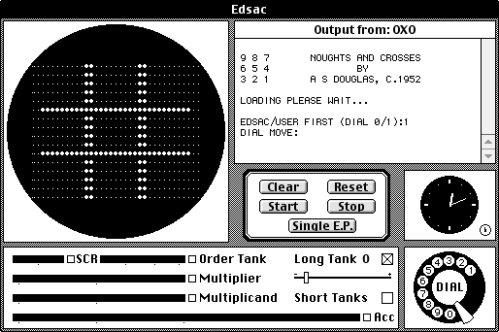
\includegraphics[scale=0.4]{oxo.png}
	\caption{Jogo para \textit{EDSAC} \textit{OXO}~[\citenum{retro}]}
	\label{retro1}
	\end{center}
\end{figure}

\begin{figure}[h!]
	\begin{center}
	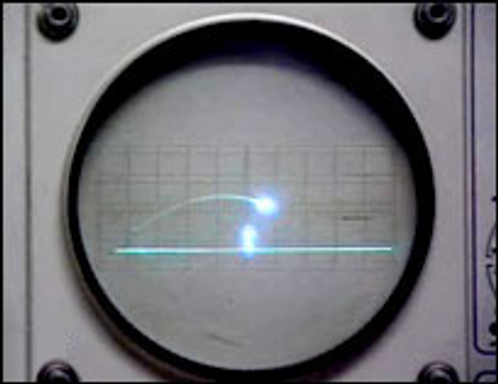
\includegraphics[scale=0.4]{tennis_for_two.jpg}
	\caption{Jogo para um oscilosc�pio \textit{Tennis for two}~[\citenum{retro}]}
	\label{retro2}
	\end{center}
\end{figure}

J� em 1962, \textit{Steve Russell} desenvolveu um jogo chamado \textit{Spacewar!} (Figura~[\ref{retro3}]), inicialmente para um sistema chamado \textit{PDP-1}. Ele consiste de um jogo de dois jogadores, cada um no controle de uma nave, em que o objetivo � atirar m�sseis para destruir a nave do oponente. O jogo conseguiu tanta popularidade que em seguida foi adaptado para v�rios outros sistemas populares na �poca, e o jogo era um teste de sistema t�o bom para o \textit{PDP-1} que o sistema era vendido j� com o jogo em mem�ria. Isso fez com que o \textit{Spacewar!} fosse o primeiro jogo de computador altamente difundido.

\begin{figure}[h!]
	\begin{center}
	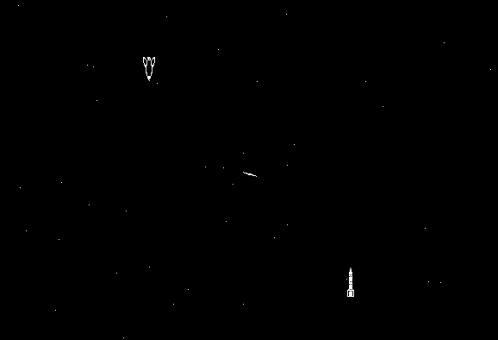
\includegraphics[scale=0.6]{spacewar.png}
	\caption{Jogo para computadores antigos \textit{Spacewars!}~[\citenum{retro}]}
	\label{retro3}
	\end{center}
\end{figure}

O primeiro console dom�stico lan�ado foi o \textit{Magnavox Odyssey}~[\citenum{odyssey}], que pode ser observado na Figura~[\ref{odyssey}], lan�ado em 1972. ele inaugurou uma id�ia inovadora, de se criar um aparelho computacional independente de uma tela, para ser conectado a televisores, algo que at� ent�o n�o havia sido pensado, os computadores sempre vinham acoplados a suas telas. Al�m disso, ele tamb�m inaugurou outro conceito que � o de m�dia remov�vel para os consoles, que evolui para os cartuchos e, hoje em dia, aos DVDs e Blu-Rays. Por�m, devido ao pre�o um pouco caro para a �poca e uma m� estrat�gia de marketing, o \textit{Odyssey} n�o foi muito popular. Uma outra companhia que inaugurou seu console em 1976, a \textit{Atari}, teve uma melhor estrat�gia. Ela lan�ou seu nome no mercado devido ao seu jogo \textit{Pong}, um simples jogo de t�nis, que foi inicialmente lan�ado para uma m�quina com uma tela que permitia o jogo atrav�s de um sistema de moedas em 1972 e foi adaptado para uma vers�o dom�stica em 1973~[\citenum{atari}]. Em 1976, utilizando um novo processador barato na �poca, o \textit{MOS 6502}, a \textit{Atari} lan�a seu primeiro console dom�stico com possiblidade de trocar jogos, o \textit{Atari 2600} (Figura~[\ref{atari}]). Esse console teve um enorme sucesso de acordo com~[\citenum{atari}].

\begin{figure}[h!]
	\begin{center}
	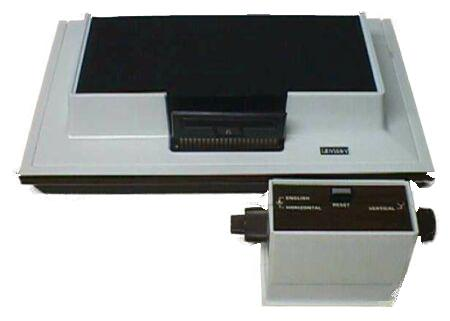
\includegraphics[scale=0.4]{odyssey.jpg}
	\caption{Console \textit{Odyssey} da \textit{Magnavox}~[\citenum{odyssey}]}
	\label{odyssey}
	\end{center}
\end{figure}

\begin{figure}[h!]
	\begin{center}
	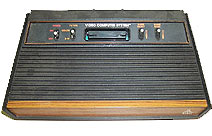
\includegraphics[scale=1.0]{atari.jpg}
	\caption{Console \textit{Atari 2600} da \textit{Atari}~[\citenum{atari}]}
	\label{atari}
	\end{center}
\end{figure}

Ambos esses consoles dom�sticos tinham controladores para se entrar o \textit{input} do jogo, o do \textit{Odyssey} sendo composto de duas rodas e um bot�o \textit{reset}, e o do \textit{Atari} sendo composto de um \textit{joystick}, que � uma haste que pode ser movida para enviar dire��es ao jogo, e um bot�o.

Ap�s esse per�odo, os \textit{video games} passaram por um decl�nio, e somente por 1980 que a \textit{Nintendo} resgatou esse mercado com o lan�amento de um jogo conhecido como \textit{Donkey Kong}, inicialmente desenvolvido em conjunto com a \textit{Atari} mas uma diverg�ncia sobre direitos autorais do \textit{Donkey Kong} fez as companhias terminarem a parceria~[\citenum{atari}]. Em 1985 a \textit{Nintendo} lan�ou seu console, o \textit{NES} (Figura~[\ref{nes}]), e passou a dominar o mercado, com pouca competi��o de sua nova concorrente, \textit{SEGA}, e seu console \textit{Master System}. Esses consoles possuiam \textit{gamepads} para a movimenta��o nos jogos, sendo compostos de uma cruz direcional que funciona similar ao joystick e v�rios bot�es.

\begin{figure}[h!]
	\begin{center}
	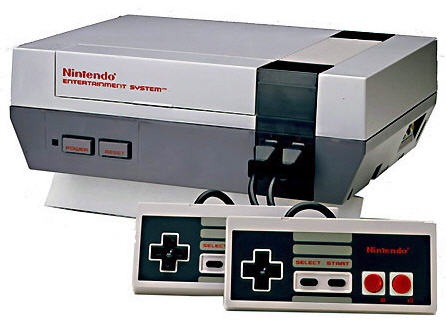
\includegraphics[scale=0.4]{nes.jpg}
	\caption{Console \textit{NES} da \textit{Nintendo}~[\citenum{nes}]}
	\label{nes}
	\end{center}
\end{figure}

Nesse momento a ind�stria do entretenimento eletr�nico teve um grande crescimento, abrindo o mercado para cada vez mais competidores a medida que se foi evoluindo as gera��es de consoles. A \textit{Nintendo} se manteve forte por todo esse tempo, se tornando uma das tr�s companhias que dominam esse mercado hoje em dia. Sua principal competidora, a \textit{SEGA}, n�o conseguiu acompanhar, e seu �ltimo console, o \textit{Dreamcast}, teve pouca venda. Atualmente a \textit{SEGA} ainda � uma empresa grande, mas ela somente faz jogos para outros consoles.

Durante a evolu��o dos jogos, uma empresa fez parceria com a \textit{Nintendo} para tentar lan�ar um novo sistema em que os cartuchos seriam trocados por CDs, diminuindo seu custo e aumenta a sua capacidade de armazenamento. Essa empresa � a \textit{Sony}. Devido a desentendimentos, a parceria terminou, mas a \textit{Sony} insistiu na id�ia e em 1994 lan�ou o seu console, o \textit{Playstation}. Esse console foi um sucesso de vendas enorme, mas o que realmente colocou a \textit{Sony} no mapa dos consoles foi o seu pr�ximo console, \textit{Playstation 2}. Esse console foi uma grande revolu��o no seu tempo e saiu um ano antes dos consoles de sua gera��o, o que ocasionou no maior �ndice de vendas de um console de \textit{video game} de todos os tempos, vendendo mais de 140 milh�es de unidades. Atualmente a \textit{Sony} compete no mercado como uma das maiores empresas de divers�o eletr�nica.

Outra empresa que resolveu explorar esse mundo dos consoles � a \textit{Microsoft}. Gigante no mundo da computa��o, ela viu a oportunidade de aplicar seus conhecimentos para criar um sistema barato, eficiente e inovador. Em 2001, ela lan�ou seu primeiro console, o \textit{Xbox}. Esse console, que � da mesma gera��o que o \textit{Playstation 2}, saiu um pouco tarde, afetando bastante as suas vendas. Ele foi feito baseado na arquitetura de um PC tradicional, mas por possuir uma produ��o muito cara, ele acabou dando altas perdas iniciais para a empresa. Por�m, a \textit{Microsoft} insistiu nesse mercado e hoje compete com as outras duas empresas por essa gera��o de consoles.

Todos esses consoles utilizaram o mesmo m�todo de input de seus predecessores, com o uso do \textit{gamepad} como entrada principal de \textit{input}, alguns possuindo outros controladores, como pistolas que poderiam apontar para a tela, mas devido ao alto pre�o desses controladores e baixa quantia de jogos compat�veis, nenhum deles chegou a fazer alguma marca no mercado.

Atualmente, o mercado dos jogos eletr�nicos conta com tr�s consoles competindo pelo mercado, o \textit{Nintendo Wii} da \textit{Nintendo}, o \textit{Xbox 360} da \textit{Microsoft} e o \textit{Playstation 3} da \textit{Sony}, os tr�s podem ser observados na Figura~[\ref{consoles}], al�m dos tr�s estarem competindo com jogos desenvolvido para os computadores pessoais, que hoje em dia existem em muitas resid�ncias, e aparelhos dos mais variados como celulares com tela sens�vel ao toque. Nesse mercado de competi��o, para ser levado em considera��o, deve-se ser inovador.

\begin{figure}[h!]
	\begin{center}
	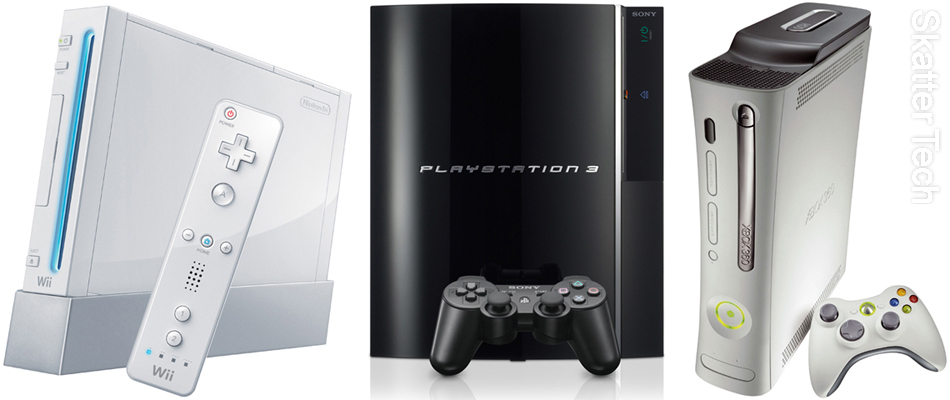
\includegraphics[scale=1.4]{wii-ps3-xbox360.jpg}
	\caption{Consoles de �ltima gera��o. Da esquerda pra direita: \textit{Wii}, \textit{Playstation 3} e \textit{Xbox 360}~[\citenum{consoles}]}
	\label{consoles}
	\end{center}
\end{figure}

Durante a evolu��o natural da intera\c{c}\~ao entre o homem e a m\'aquina, busca-se cada vez mais a adapta\c{c}\~ao dos gestos para o ambiente virtual. Ao fornecer ao usu\'ario gestos f\'aceis de se usar, se diminui a curva de aprendizado para se utilizar algo, bem como mant\^em um ambiente mais familiar ao usu\'ario. As grandes companhias competidoras j� est�o caminhando em dire��o a isso. O \textit{Nintendo Wii} possui controles sens�veis ao movimento, permitindo o uso de gestos para o controle em seus jogos, o \textit{Wiimote} (Figura~[\ref{wiimote}]), assim como o \textit{Playstation 3} possui seus controles sens�veis ao movimento e com no��o de profundidade, o \textit{Playstation Move} (Figura~[\ref{move}]), e o \textit{Xbox 360} possui o \textit{Kinect} (Figura~[\ref{kinect}]), uma c�mera inteligente capaz de identificar gestos.

\begin{figure}[h!]
	\begin{center}
	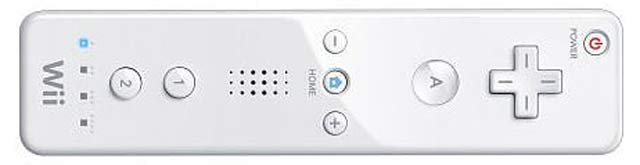
\includegraphics[scale=0.2]{wiimote.jpg}
	\caption{Controle para \textit{Nintendo Wii} \textit{Wiimote}~[\citenum{controles}]}
	\label{wiimote}
	\end{center}
\end{figure}

\begin{figure}[h!]
	\begin{center}
	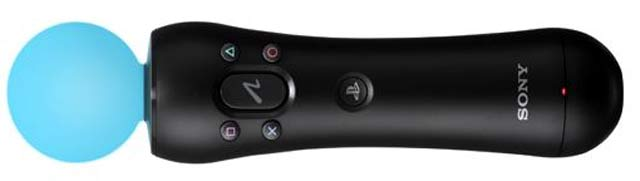
\includegraphics[scale=0.2]{move.jpg}
	\caption{Controle para \textit{Playstation 3} \textit{Playstation Move}~[\citenum{controles}]}
	\label{move}
	\end{center}
\end{figure}

\begin{figure}[h!]
	\begin{center}
	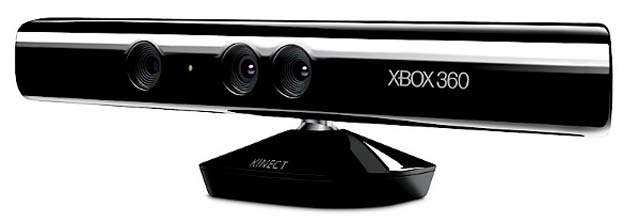
\includegraphics[scale=0.2]{kinect.jpg}
	\caption{C�mera para \textit{Xbox 360} \textit{Kinect}~[\citenum{controles}]}
	\label{kinect}
	\end{center}
\end{figure}

Como apresentado anteriormente, os consoles principais disputam o mercado de jogos com v�rios aparelhos diferentes. Um desses aparelhos que ainda � pouco explorado trata de mesas com superf�cie multi-toque. Tem poucos exemplos de mesas multi-toque, como a \textit{Reactable}~[\citenum{react}] ou a \textit{Microsoft Surface}~[\citenum{microsoftsurface}], e nenhuma que j� esteja popularmente dispersada no mercado, devido ao alto custo que as op��es comerciais normalmente possuem. Esta interface, no entanto, possui um grande potencial, e existem alternativas para construir mesas deste tipo usando materiais baratos, o que foi feito no decorrer deste trabalho.

Estas mesas multi-toque j� possuem alguns \textit{softwares} dispon�veis, por�m n�o existe um bom software que demonstre inteiramente as capacidades de \textit{input} da mesa. Dessa forma, este trabalho mostra a cria��o de um software simulador de f�sica bidimensional para uma mesa com superf�cie multi-toque, que devido as suas propriedades possui uma boa sinergia com o m�todo de interface escolhido, explorando assim, as capacidades de \textit{input} da mesa em um �nico \textit{software} de estilo pouco explorado e divertido.

Os softwares simuladores de f�sica s�o essencialmente programas em que se come�a com um mundo em aberto, e o usu�rio pode desenhar nele os objetos que desejar, podendo atribuir a eles as propriedades que quiser, e eles ir�o se interagir de acordo com as leis da f�sica, obedecendo gravidade, acelera��o e empuxo. Assim, um software nesse estilo permitiria utilizar as capacidades da mesa demonstrando seus gestos dispon�veis, como scale e rotate, bem como a detec��o de gestos padr�es como o desenho de um quadrado ou c�rculo. Softwares nesse estilo incluem o \textit{Phun}, \textit{Crayon Physics} e \textit{Numpty Physics}, este �ltimo que possui uma convers�o para \textit{input} multi-toque, por�m ele possui recursos limitados e n�o foi planejado para corretamente suportar um n�mero arbrit�rio de toques vindo de um n�mero desconhecido de usu�rios, o que deve ser cuidado ao se desenvolver softwares para uma mesa multi-toque.

O software desenvolvido neste trabalho, chamado de \textit{Deskworld}, segue estas mesmas regras de softwares simuladores de fisica, por�m, como � planejado para mesas multi-toque, possui algumas propriedades novas, como a possibilidade de se dividir o mundo para utiliza��o de usu�rios em condi��es diferentes, e a detec��o de gestos para aproximar formas ao seu estado ideal, pois � dif�cil de se desenhar algo preciso utilizando somente os dedos.

Como as mesas com tela multi-toque n�o s�o ainda dispon�veis em massa para a resid�ncia dos usu�rios, sua maior taxa de uso est� focada em exposi��es, onde os usu�rios possuem somente um encontro breve com a mesa. Assim, um aplicativo desenvolvido para uma mesa dessas necessita ser f�cil de se utilizar e possuir suporte a m�ltiplos usu�rios a interagindo simult�neamente a qualquer momento, o que � feito com o software desenvolvido neste trabalho. Ao mesmo tempo, este software possui uma grande capacidade de cria��o, proporcionando tamb�m divers�o para usu�rios a longo prazo.

O restante deste trabalho est� dividido conforme segue. O segundo cap�tulo deste trabalho apresenta trabalhos correlatos, exibindo mesas parecidas a desenvolvida e \textit{softwares} similares ao proposto, ambos para mesas como para outros sistemas em geral, sens�veis ao toque ou n�o. O terceiro cap�tulo apresenta o fundamento te�rico por tr�s da mesa, explicando os princ�pios de processamento de imagem necess�rios para se entender os toques na mesa, bem como os filtros utilizados, e explica os m�todos de ilumina��o e como isso afeta este projeto. O quarto cap�tulo detalha sobre a constru��o da mesa em si, onde est� exposto o projeto da mesa, explicando as decis�es de \textit{hardware} escolhidos de acordo com as dimens�es da mesa e explicando como foram feitos fisicamente os passos necess�rios para a detec��o de toque, com a utiliza��o de LEDs e uma c�mera infravermelha. O quinto cap�tulo demonstra a implementa��o do \textit{software} proposto, chamado \textit{Deskworld}, apresentando aspectos como o \textit{Design} que explica seus detalhes, conceito, objetos e regras. Neste mesmo cap�tulo � exibido a arquitetura utilizada, detalhes de implementa��o, mostrando como foi implementado em uma vis�o de n�vel mais baixo, explicando as decis�es do projeto e as escolhas feitas sobre a orienta��o a componentes. Na se��o final deste cap�tulo, explica-se com mais detalhes sobre as ferramentas utilizadas de suporte para a implementa��o do jogo proposto, como a Touchlib e a engine Box2D. Por fim, o sexto cap�tulo elenca algumas considera��es finais e trabalhos futuros.
\chapter{Trabalhos Correlatos}
\label{cap2}
Neste cap�tulo, primeiramente s�o expostos os principais trabalhos relativos a implementa��es de mesas com superf�cies multi-toque. Em seguida, no intuito de demonstrar o potencial deste tipo de interface, s�o apresentados uma s�rie de \textit{softwares} interativos, incluindo jogos, desenvolvidos para mesas multi-toque. Ao final s�o mostrados alguns \textit{softwares} simuladores de f�sica em geral, para diversos sistemas, incluindo mesas com superf�cie multitoque.

\section{Mesas com superf�cie multi-toque}
\label{cap2.1}
As mesas com superf�cie multi-toque s�o relativamente recentes no mercado, por�m seu alto custo fez com que n�o fossem muito proliferadas. Devido a isto, alternativas foram feitas para constru��o de mesas de baixo custo. Uma alternativa criativa foi proposta por~[\citenum{mtmini}], onde demonstra-se a viabilidade da montagem de uma pequena mesa com superf�cie multitoque com menos de US\$50,00. Com materiais de baixo custo como papel�o, papel e vidro, construiram uma mesa utilizando um computador pessoal e uma \textit{webcam}. Outras alternativas artesanais incluem, por exemplo, a constru�da para o jogo \textit{Eco-Defense}~[\citenum{pedrosaulo}], a elaborada para o jogo \textit{IRTaktiks}~[\citenum{IRTaktiks}], bem como a \textit{Virttable}~[\citenum{virttable}].

Diversas utilidades s�o propostas para essas mesas. Tem-se por exemplo a \textit{Reactable}~[\citenum{react}] (Figura~\ref{react}), dispon�vel desde 2008, que, apesar de n�o possibilitar o toque do usu�rio, utiliza marcadores fiduciais para habilitar a intera��o de seus usu�rios com a m�sica, fornecendo um instrumento musical diferente. Ela � utilizada em concertos e eventos.

\begin{figure}[h!]
	\begin{center}
	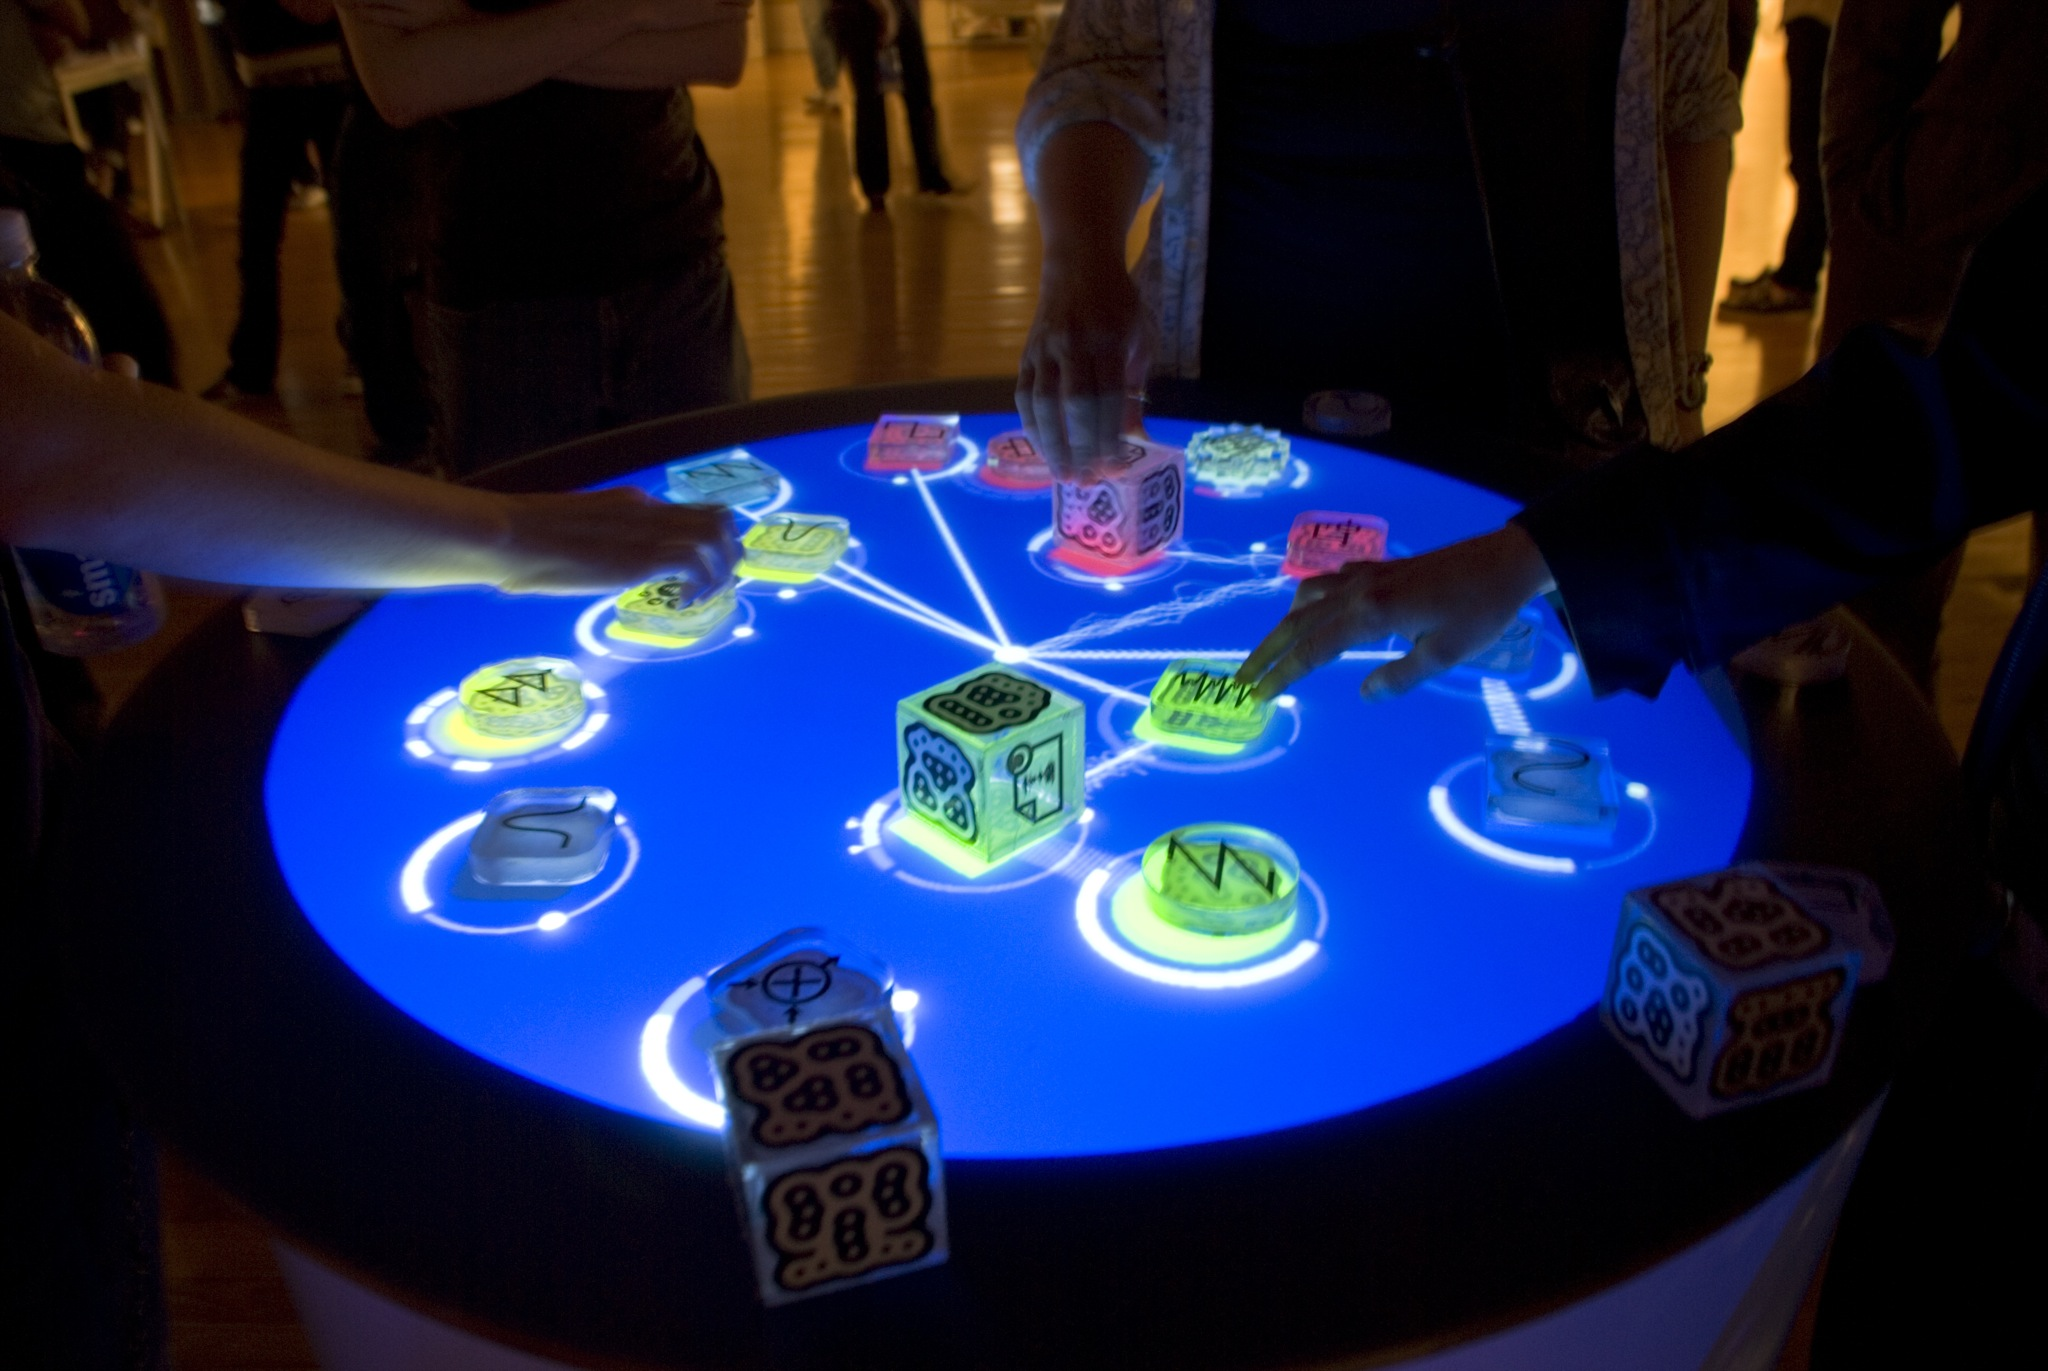
\includegraphics[scale=0.60]{reactable.jpg}
	\caption{\textit{Reactable} - Mesa com marcadores fiduciais~[\citenum{react}]}
	\label{react}
	\end{center}
\end{figure}

Outro exemplo � a \textit{Microsoft Surface}~[\citenum{microsoftsurface}] (Figura~\ref{msurface}), que proporciona funcionalidades diversas, tais como a habilidade de compartilhar figuras e arquivos por meio da intera��o com objetos eletr�nicos colocados sobre sua superf�cie e comandos via o toque do usu�rio. 

\begin{figure}[h!]
	\begin{center}
	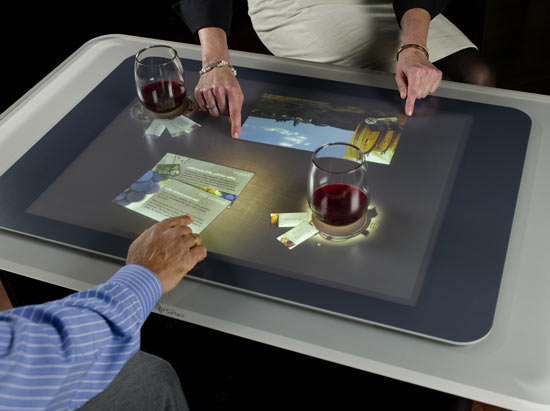
\includegraphics[scale=0.60]{microsoft_surface_main.jpg}
	\caption{\textit{Microsoft Surface}~[\citenum{microsoftsurface}]}
	\label{msurface}
	\end{center}
\end{figure}

Essas duas mesas s�o as mais populares, apesar de existirem outros projetos comerciais e desenvolvidos para exibi��es, como a \textit{Touch Magix}~[\citenum{Touchmagix}] ou a desenvolvida pela companhia \textit{Ideum}, visto em~[\citenum{ideum}].

A id�ia presente em todas � a mesma, ou seja, utilizar um projetor multim�dia para projetar a imagem na superf�cie da mesa, na qual o usu�rio pode tocar para interagir com o \textit{software}. A superf�cie � iluminada com a utiliza��o de \textit{LED}s (\textit{Light-emitting diode}) e os toques s�o detectados por uma c�mera sem filtro infravermelho que os interpreta em rela��o � posi��o na mesa. Existem v�rias maneiras de iluminar uma mesa. As principais s�o DI (\textit{Diffuse Ilumination}) e FTIR (\textit{Frustrated Total Internal Reflection}).

\begin{figure}[h!]
	\begin{center}
	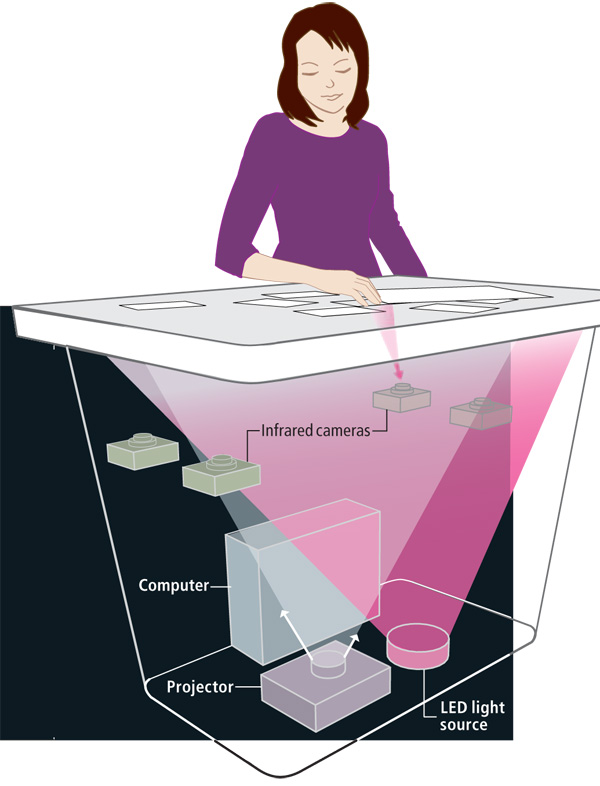
\includegraphics[scale=0.40]{touch_table.jpg}
	\caption{Projeto de mesa multitoque com DI~[\citenum{scient}]}
	\label{touchtable}
	\end{center}
\end{figure}

A ilumina��o por DI, ilustrada na Figura~\ref{touchtable}, refere-se aos \textit{LED}s que iluminam a mesa por baixo do acr�lico. Esse m�todo � utilizado, por exemplo, na \textit{Microsoft Surface}~[\citenum{microsoftsurface}] e na mesa constru�da para o jogo \textit{Eco-Defense}~[\citenum{pedrosaulo}].

O outro m�todo de ilumina��o � o FTIR, acompanhado na Figura~\ref{FTIR}. Nesta t�cnica, os LEDS s�o embutidos no acr�lico da superf�cie da mesa. Assim, a luz proveniente dos LEDs sofre de um fen�meno denominado reflex�o interna total frustada. Isso significa que a ilumina��o fica retida dentro do acr�lico sem conseguir sair. Ao momento que um dedo toca na superf�cie, a capacidade de refra��o da superf�cie muda, o que permite que a luz saia e ilumine o toque, onde uma c�mera infravermelho consegue captar essa luz, detectando o local do toque. Esse tipo de detec��o � normalmente mais precisa que a detec��o por DI, pois sofre menos interfer�ncia do fundo. Entretanto, ela � inadequada no reconhecimento de marcadores fiduciais, pois dependendo do material desses marcadores, n�o h� nitidez na ilumina��o FTIR para poder identificar e distinguir as marcas se a superf�cie n�o tiver seu coeficiente de refra��o alterado.

\begin{figure}[h!]
	\begin{center}
	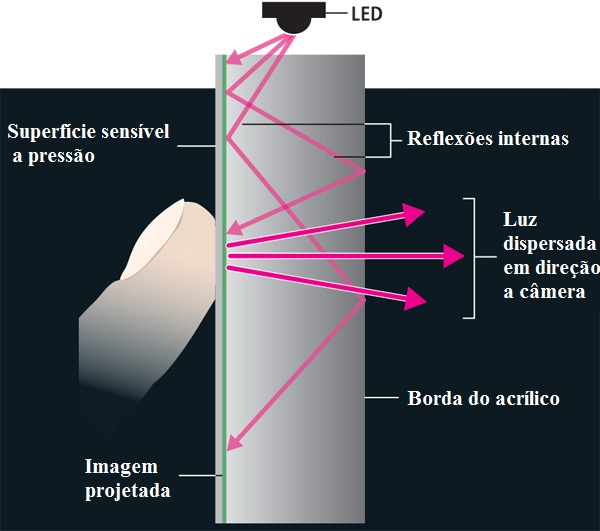
\includegraphics[scale=0.50]{touch_FTIR_port.jpg}
	\caption{Esquema de detec��o de toque FTIR (adaptada de~[\citenum{scient}])}
	\label{FTIR}
	\end{center}
\end{figure}

Outra abordagem trata da combina��o entre as duas abordagens anteriores, exemplificado pela \textit{Virttable}~[\citenum{virttable}] (Figura~\ref{virttable}), que utiliza este m�todo procurando proporcionar a melhor detec��o poss�vel de toques e marcadores fiduciais simultaneamente. Um problema desta abordagem � a interfer�ncia do fundo para a detec��o de toques, fazendo com que o ambiente no qual a mesa se encontra tenha que ser controlado para sua correta ilumina��o. No entanto, em rela��o a uma mesa com ilumina��o exclusivamente DI, os toques s�o mais bem iluminados, facilitando as detec��es.

\begin{figure}[h!]
	\begin{center}
	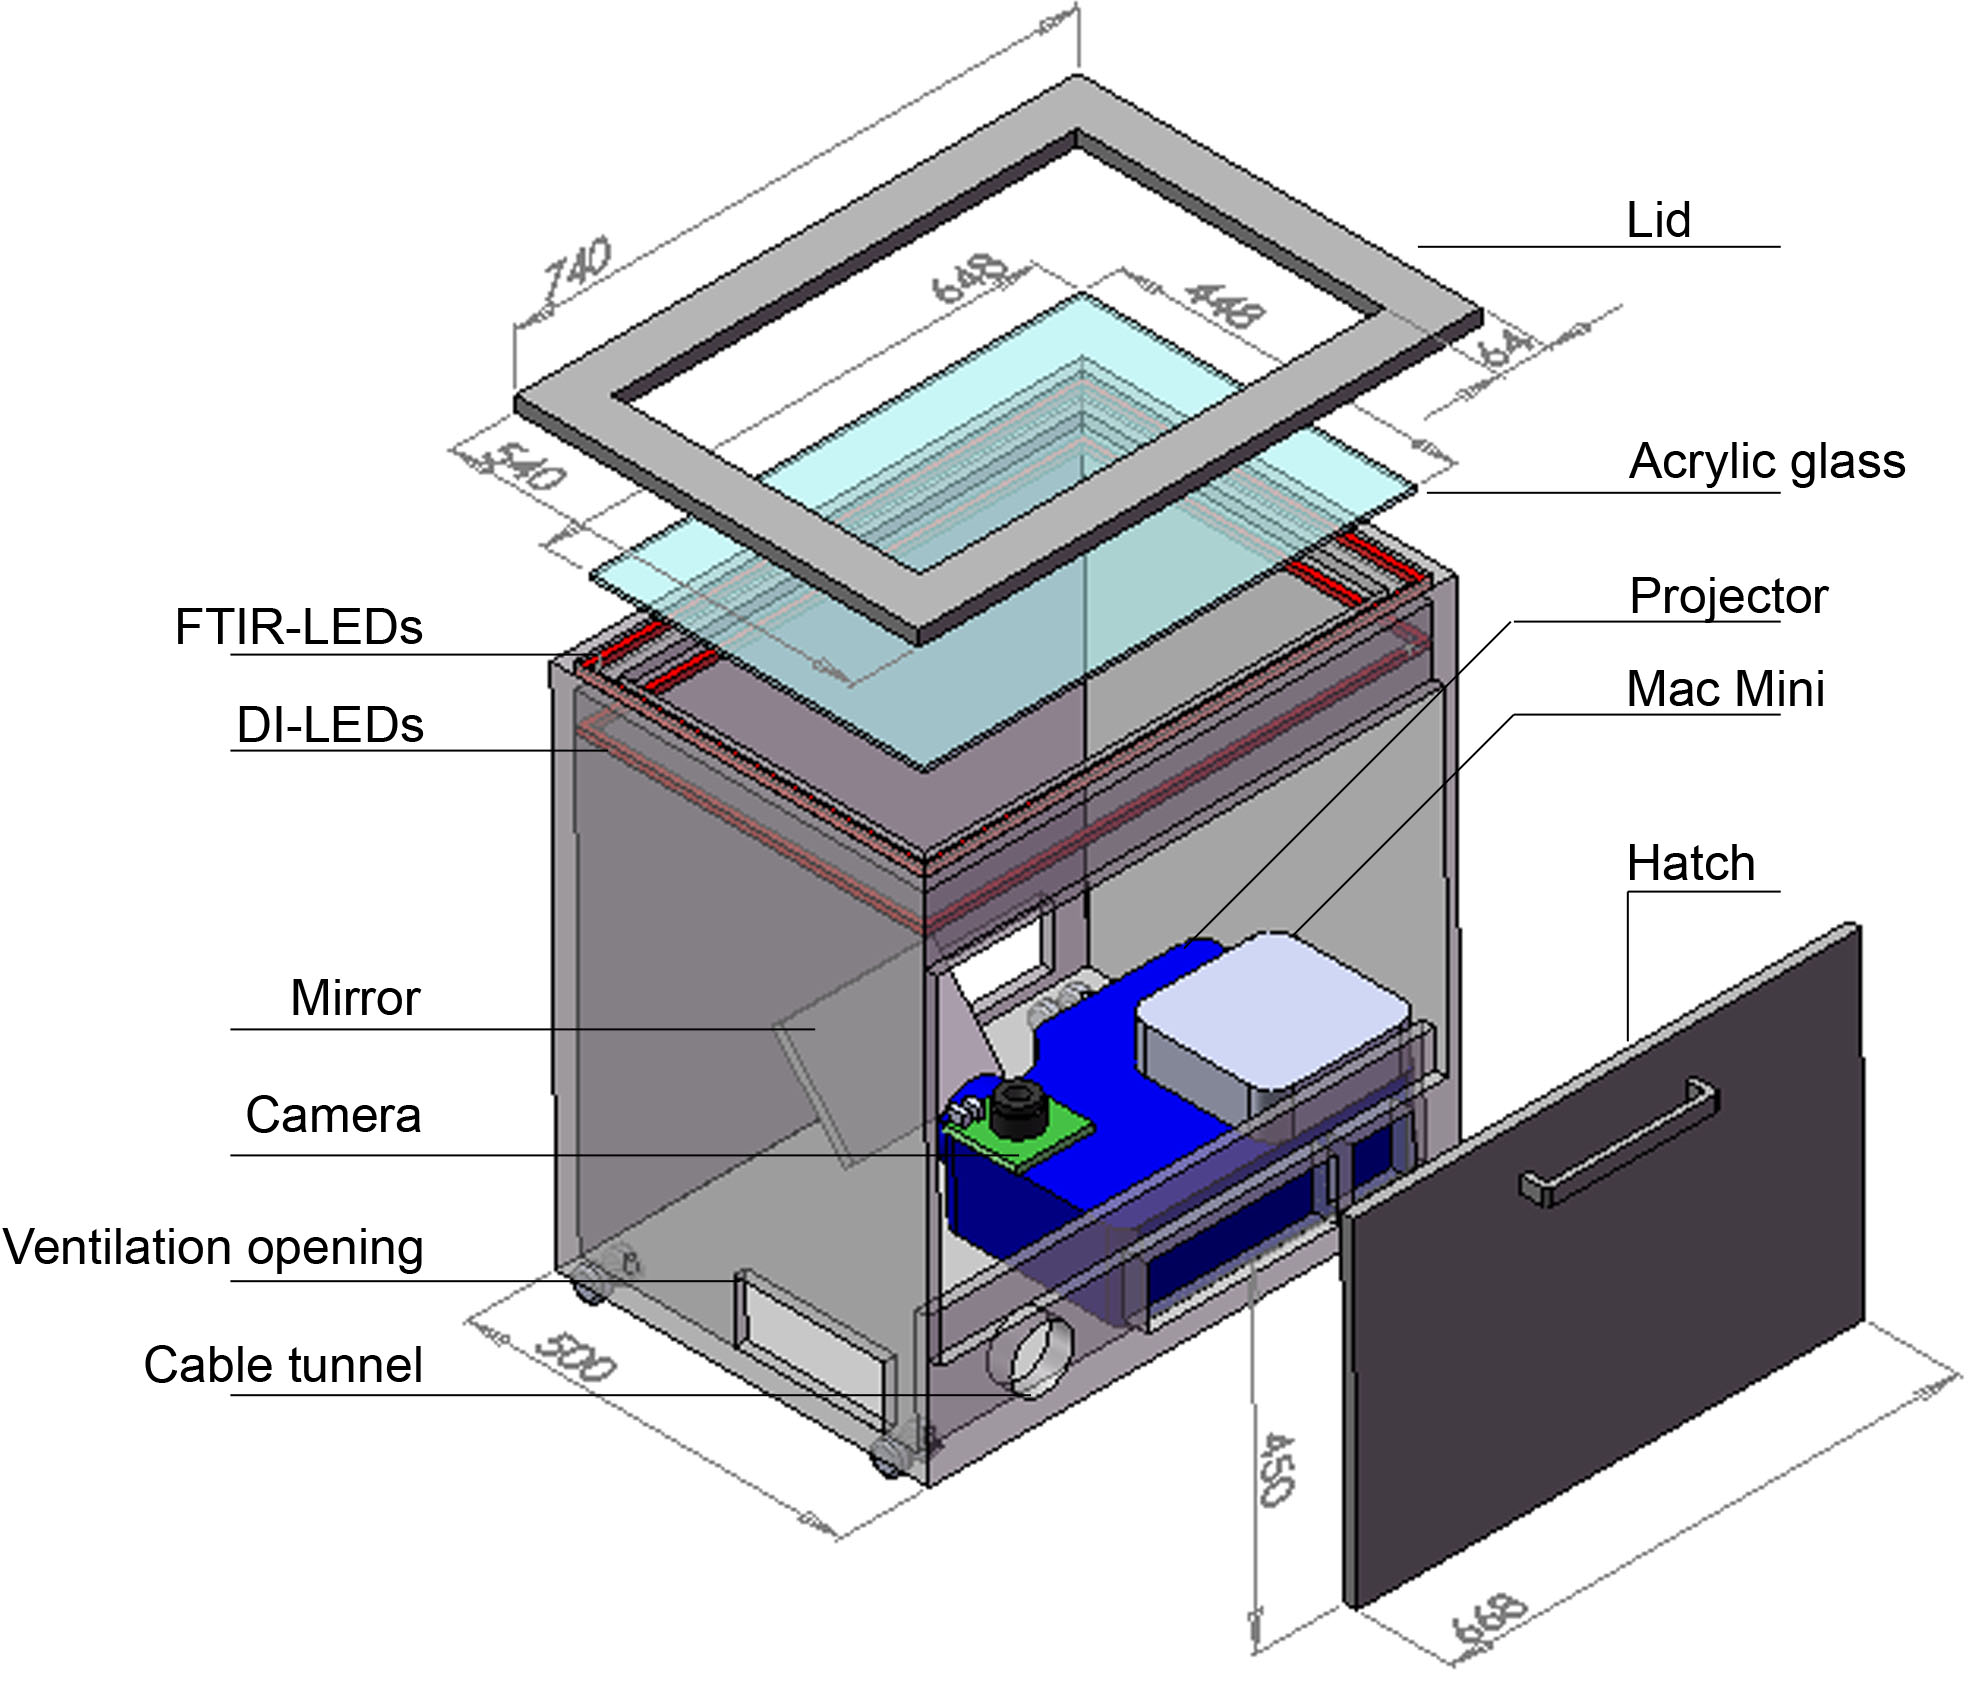
\includegraphics[scale=0.17]{virttable.jpg}
	\caption{Projeto da mesa \textit{Virttable}~[\citenum{virttable}]}
	\label{virttable}
	\end{center}
\end{figure}

\section{\textit{Softwares} interativos para mesas com superf�cie multitoque}
\label{cap2.2}

Existem v�rios \textit{softwares} produzidos para utiliza��o em mesas com superf�cie multitoque. Por exemplo, o \textit{IRTaktiks}~[\citenum{IRTaktiks}] (Figura~\ref{irtaktiks}), um jogo de estrat�gia desenvolvido para uma mesa com ilumina��o \textit{FTIR} constru�da durante o mesmo projeto. Este jogo foi desenvolvido para dois jogadores, onde cada um tem suas unidades e deve derrotar as unidades inimigas. Um problema, no entanto, � a identifica��o do jogador, pois n�o h� verifica��o a qual jogador pertence os toques feitos sobre a mesa, o que permite aos jogadores, acidentalmente ou n�o, controlar as unidades do inimigo. Al�m disso, o jogo foi projetado para apenas dois jogadores, o que n�o tira proveito da caracter�stica multiusu�rio inerente �s mesas multitoque. 

\begin{figure}[h!]
	\begin{center}
	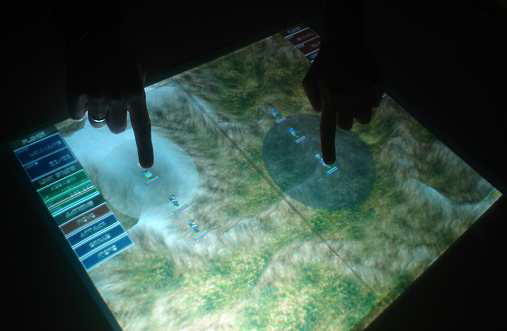
\includegraphics[scale=0.8]{irtaktiks.png}
	\caption{Jogo para mesas com superf�cie multitoque \textit{IRTaktiks}~[\citenum{IRTaktiks}]}
	\label{irtaktiks}
	\end{center}
\end{figure}

Por se tratarem de superf\'icies normalmente sem limita\c{c}\~oes de n\'umero de toques, os jogos desenvolvidos para mesas devem focar em interatividade de v\'arios jogadores. \textit{Softwares} como o \textit{The Laundry Game}~[\citenum{laundrygame}] (Figura~\ref{laundry}), que \'e um jogo de separa\c{c}\~ao de roupas em categorias, e o \textit{Game of Life} (Figura~\ref{life}), feito pelo \textit{Verve Project}~[\citenum{gameoflife}], que \'e o tradicional jogo da vida, onde uma bact\'eria vive dependendo do n\'umero de bact\'erias ao seu redor. Apesar de estes jogos serem simples, divertidos, e multiusu�rio, a limita��o das a��es poss�veis faz com que os usu�rios abandonem seu uso precocemente.

\begin{figure}[h!]
	\begin{center}
	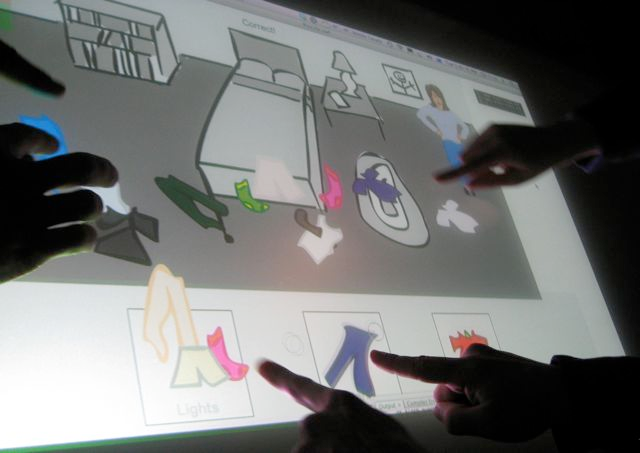
\includegraphics[scale=0.8]{laundrygame.png}
	\caption{\textit{The Laundry Game} - Jogo para mesas com superf�cie multitoque~[\citenum{laundrygame}]}
	\label{laundry}
	\end{center}
\end{figure}

\begin{figure}[h!]
	\begin{center}
	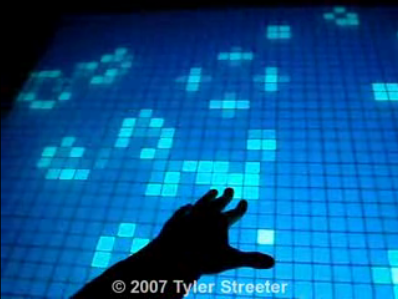
\includegraphics[scale=0.8]{gameoflife.png}
	\caption{\textit{Game of Life} - \textit{Software} para mesas com superf�cie multitoque~[\citenum{gameoflife}]}
	\label{life}
	\end{center}
\end{figure}

Outros \textit{softwares} para mesas s\~ao mais completos, possuindo graus de dificuldade e sistema de pontua\c{c}\~ao. Um desses jogos � o \textit{Eco Defense}~[\citenum{pedrosaulo}] (Figura~\ref{ecodefense}), onde o jogador deve destruir nuvens de polui\c{c}\~ao antes que elas afetem a floresta posicionada nas bordas da tela, podendo colocar torres de defesa para ajudar. O grau de dificuldade vai aumentando de acordo com o tempo de jogo, pois as nuvens ficam cada vez mais r�pidas e numerosas, at� que jogadores percam. Outro exemplo � o \textit{Station Defender}~[\citenum{multphys}] (Figura~\ref{defender}), onde os jogadores devem defender sua base construindo paredes ao redor dela. Ambos jogos proporcionam melhor jogabilidade, pois h� mudan�a no grau dificuldade e a busca pela sobreviv�ncia pelo maior tempo poss�vel envolve os jogadores, gerando competitividade.

\begin{figure}[h!]
	\begin{center}
	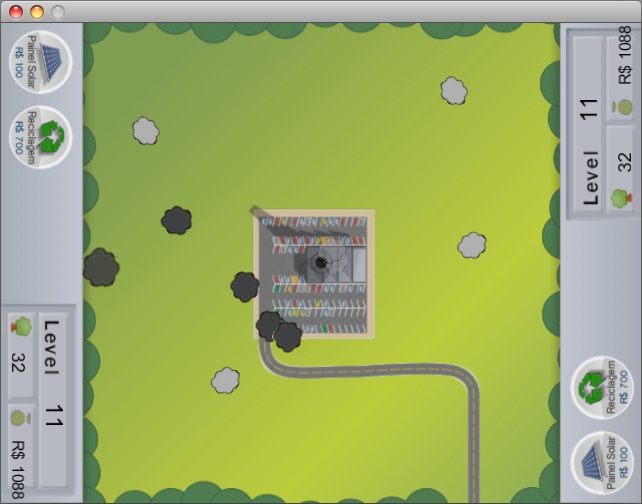
\includegraphics[scale=0.60]{ecodefense.jpg}
	\caption{\textit{Ecodefense} - Jogo para mesas com superf�cie multitoque~[\citenum{pedrosaulo}]}
	\label{ecodefense}
	\end{center}
\end{figure}

\begin{figure}[h!]
	\begin{center}
	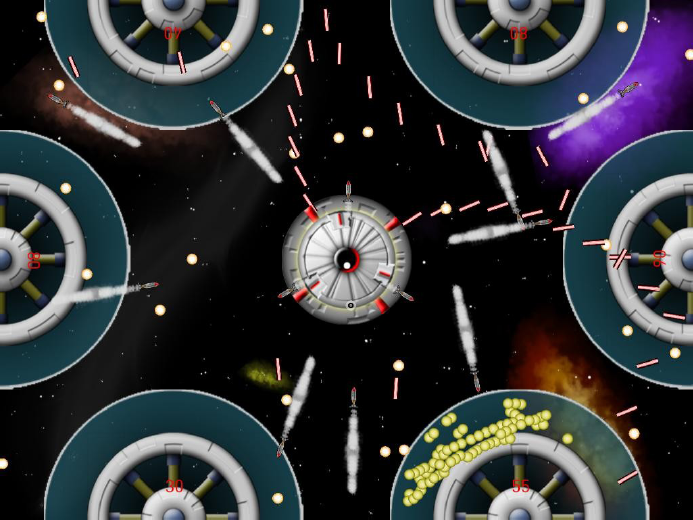
\includegraphics[scale=0.60]{stationdefender.png}
	\caption{\textit{Station Defender} - Jogo para mesas com superf�cie multitoque~[\citenum{multphys}]}
	\label{defender}
	\end{center}
\end{figure}

\section{\textit{Softwares} simuladores de f�sica}
\label{cap2.3}
Um \textit{software} simulador de f�sica consiste de um programa que possui um mundo aberto onde o usu�rio pode criar o que desejar. Estas cria��es recebem propriedades de um objeto tradicional e interagem com o mundo de acordo com as leis da f�sica.

Um jogo que abriu as portas para a populariza��o desse tipo de \textit{software}� o \textit{Little Big Planet}~[\citenum{lbp}] (Figura~\ref{lbp}). Nesse jogo, inicialmente desenvolvido para \textit{Playstation 3}~[\citenum{ps3}] e depois para \textit{Playstation Portable}~[\citenum{psp}], o jogador controla um boneco chamado \textit{Sack Boy}, que pode mudar sua apar�ncia como quiser, e deve seguir por uma fase no estilo de jogo de plataforma at� chegar ao seu final. A diferen�a est� no tipo do jogo, que os criadores chamaram de \textit{Play, Create, Share}, onde os jogadores s�o livres para criar suas pr�prias fases como quiserem, compartilhando-as com todos os outros jogadores do mundo. Neste modo, o \textit{Sack Boy} pode colocar objetos em jogo para construir a fase, e os objetos interagem de acordo com as leis da f�sica, podendo possuir movimento e atrapalhar ou ajudar uns aos outros, podendo ser perigosos ou n�o para o \textit{Sack Boy}. Com esta ferramenta, os jogadores constru�ram in�meras fases inovadoras ao redor do mundo, inventando coisas que at� os criadores nunca haviam imaginado. O sucesso foi tanto que os criadores do \textit{Little Big Planet} lan�aram recentemente a sua continua��o, \textit{Little Big Planet 2}~[\citenum{lbp2}], onde a cria��o de fases vai al�m de jogos de plataforma como na primeira vers�o, com a possibilidade do jogador criar regras no jogo que permitam a cria��o de v�rios tipos de jogos diferentes, como por exemplo, jogos do tipo \textit{shooter} ou de estrat�gia.

\begin{figure}[h!]
	\begin{center}
	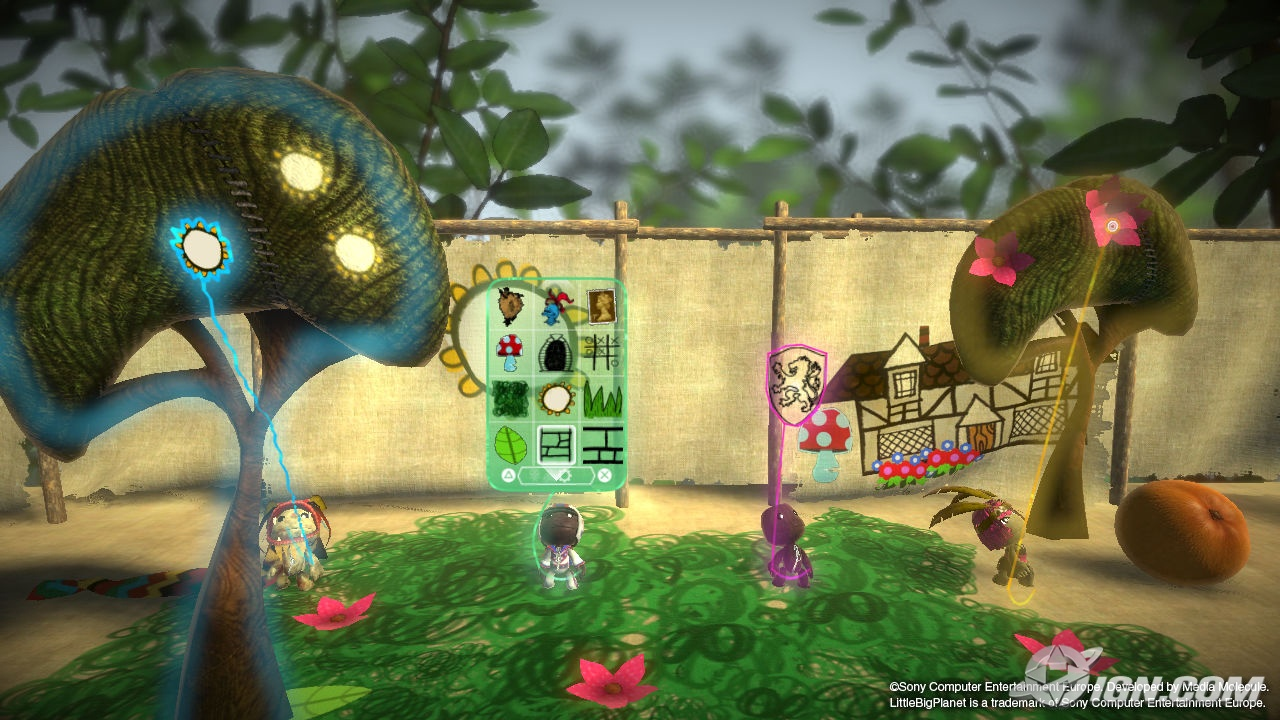
\includegraphics[scale=0.30]{lbp.jpg}
	\caption{\textit{Little Big Planet} - Jogo para \textit{PS3}~[\citenum{lbp}]}
	\label{lbp}
	\end{center}
\end{figure}

Ainda dentro da categoria de \textit{Play, Create, Share}, a mesma empresa criadora do \textit{Little Big Planet} lan�ou o jogo \textit{Modnation Racer}~[\citenum{mdr}] (Figura~\ref{modnation}), um jogo de corrida onde os jogadores podem criar as suas pr�prias pistas de corridas e compartilhar com todos os demais. Lan�ado em maio de 2010, j� possui milhares de pistas criadas por usu�rios. Esses jogos demonstram a popularidade do estilo onde o usu�rio � quem cria seu pr�prio jogo.

\begin{figure}[h!]
	\begin{center}
	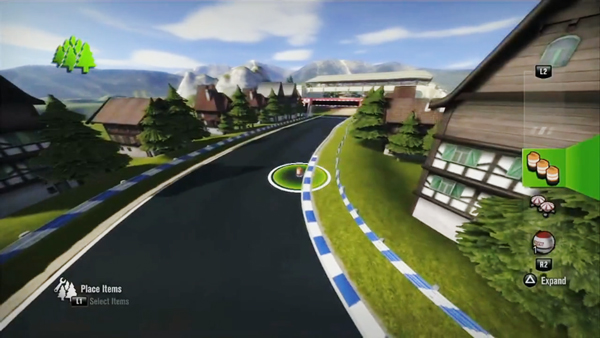
\includegraphics[scale=0.70]{modnation.jpg}
	\caption{\textit{Modnation Racer} - Jogo para \textit{PS3}~[\citenum{lbp}]}
	\label{modnation}
	\end{center}
\end{figure}

No cen�rio de \textit{softwares} simuladores de f�sica 2D, existe um \textit{software} chamado \textit{Phun}~[\citenum{phun}] (Figura~[\ref{phun}]), que n�o possui objetivo. Ele � uma ferramenta simuladora de f�sica 2D que permite ao usu�rio construir o ambiente que desejar, podendo desenhar formas geom�tricas tradicionais ou livres, modificar a taxa de gravidade e a fric��o dos objetos, transformar objetos para forma l�quida e controlar densidade dos elementos, entre outros.

\begin{figure}[h!]
	\begin{center}
	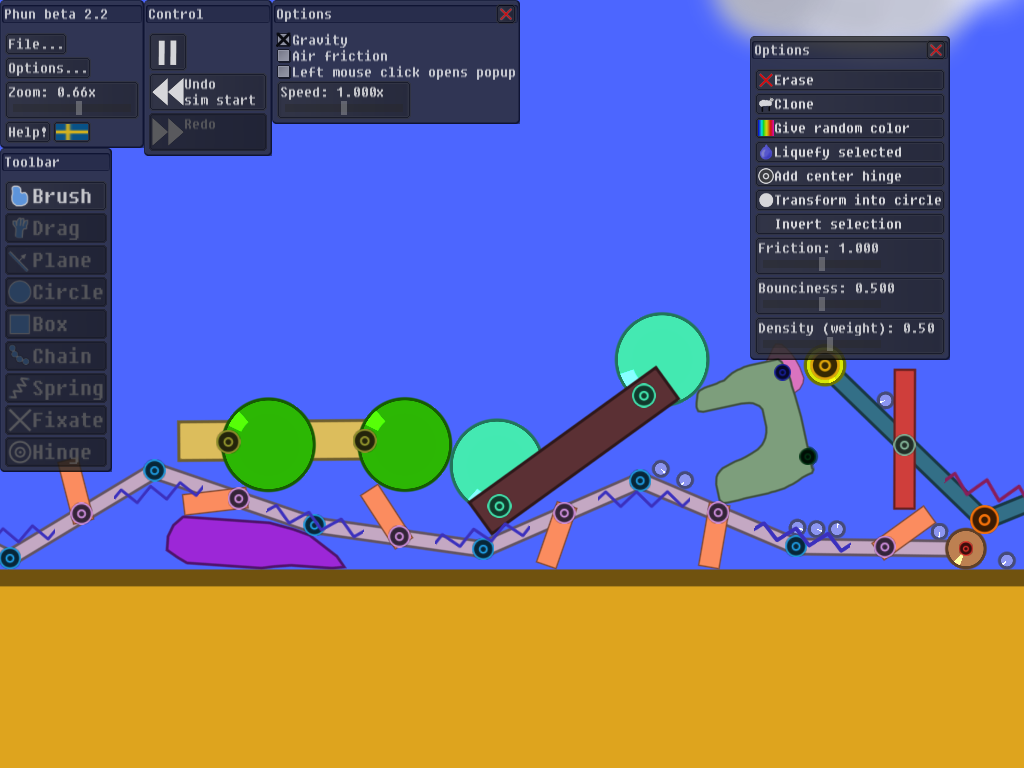
\includegraphics[scale=0.40]{Phun.jpg}
	\caption{\textit{Phun} - Jogo para PC~[\citenum{phun}]}
	\label{phun}
	\end{center}
\end{figure}

Um jogo muito popular neste estilo � o \textit{Crayon Physics}~[\citenum{crayonphysics}]. Neste jogo, � apresentado ao jogador um cen�rio que possui uma bola e inicialmente uma estrela. O jogador deve guiar a bola de modo a coletar todas as estrelas que lhe s�o apresentadas para completar a fase. Para isso, o jogador possui um giz de cera virtual e deve-se com ele modificar livremente o cen�rio, podendo desenhar a forma que quiser, adicionando-a ao mundo assim que ele acabar de desenh�-la. Uma vez no mundo, o objeto obedece a gravidade e adquire um momento, obtendo assim um movimento. O jogador ainda pode utilizar pontos de fixa��o para prender objetos juntos e correntes para fazer dispositivos improvisados como elevadores. Tudo isso � feito levando-se em conta as leis da f�sica, como as tr�s leis de \textit{Newton} aplicadas a um mundo bidimensional. Este jogo foi adaptado para mesas com superf�cie multitoque utilizando \textit{Action Script} por um grupo chamado \textit{Multitouch Barcelona}~[\citenum{barcelonamultcrayon}]. Contr�rio a sua inspira��o original, ele possui somente o modo de cria��o do \textit{Crayon Physics}, n�o tendo objetivo e por isso n�o pode ser chamado de jogo.

\begin{figure}[h!]
	\begin{center}
	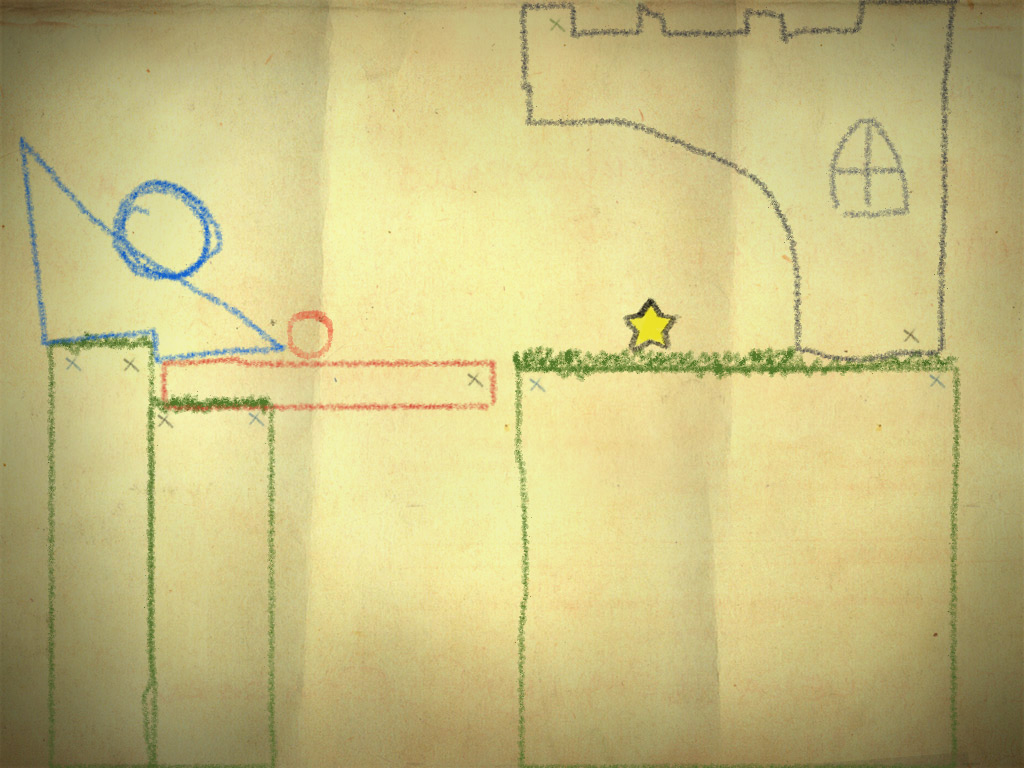
\includegraphics[scale=0.30]{crayon.jpg}
	\caption{\textit{Crayon Physics}- Jogo para PC~[\citenum{crayonphysics}]}
	\label{crayon}
	\end{center}
\end{figure}

Inspirado no \textit{Crayon Physics}, foi desenvolvido o \textit{Numpty Physics}~[\citenum{numptyphysics}] cujos objetivo e ferramentas s�o os mesmos do seu precursor, com a vantagem de possuir c�digo aberto. Este jogo foi adaptado para funcionar em mesas com superf�cies multitoque, a partir de um trabalho de gradua��o da Universidade T�cnica de Viena~[\citenum{multnump}]. Nesta adapta��o, al�m das fases existentes no \textit{Numpty Physics}, foram inclu�das seis novas fases com uma bola adicional, permitindo a participa��o de um segundo jogador, como pode ser observado na Figura~\ref{numpty}. No entanto, este jogo apresentou-se inst�vel, pois � suscet�vel a erros de execu��o.

\begin{figure}[h!]
	\begin{center}
	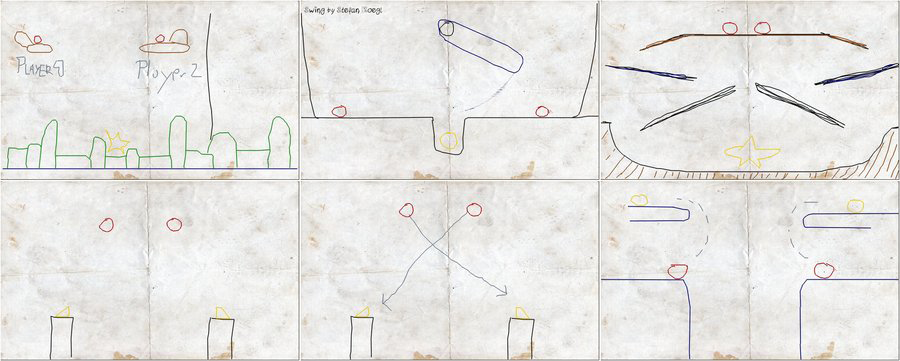
\includegraphics[scale=0.6]{numpty.png}
	\caption{Seis fases adicionais da adapta��o do \textit{Numpty Physics} para mesas multitoque.~[\citenum{multnump}]}
	\label{numpty}
	\end{center}
\end{figure}

Neste cap�tulo foi poss�vel observar o pot�ncial de cria��o livre e independente que os \textit{softwares} simuladores de f�sica apresentam. Al�m disso, s�o intuitivos e podem ter sua intera��o fortemente melhorada se implementados para uma interface sens�vel ao toque. Em termos de usabilidade, neste tipo de interface, \textit{softwares} simuladores f�sica podem ser implementados para m�ltiplos usu�rios interagindo simultaneamente. Contudo, dentre os trabalhos desenvolvidos e analisados, n�o existem \textit{softwares} simuladores de f�sica desenvolvidos para mesas com superf�cie multi-toque que apresentem implementa��es robustas e satisfat�rias.

\chapter{Fundamenta��o Te�rica}
\label{cap3}

Tradicionalmente, existe a pr�tica de implementar jogos e outros \textit{softwares} direcionados a um �nico usu�rio. Algumas iniciativas at� consideram dois ou mais usu�rios, por�m, cada um realizando seu \textit{input} via teclado, \textit{joystick} ou \textit{mouse}. \textit{Softwares} desenvolvidos para superf�cies multitoque, no entanto,  possuem um paradigma diferente, sendo fundamental o desenvolvimento de suporte a um n�mero indeterminado de usu�rios, que podem compartilhar uma �nica superf�cie multitoque por meio da qual � realizado \textit{input} simult�neo. Por isso s�o utilizadas t�cnicas diferentes para reconhecimento de cada toque e para o processamento das imagens que traduzem cada \textit{input}.

Neste cap�tulo s�o apresentadas as t�cnicas para detec��o de toques. Ou seja, � detalhado como as imagens obtidas pela c�mera s�o processadas para detec��o da forma��o e movimenta��o de \textit{blobs}(\textit{Bright Luminescent Objects}) que correspondem aos toques e gestos sobre a mesa. Este processamento envolve a aplica��o de filtros, al�m da corre��o da imagem para eliminar a distor��o. Tamb�m s�o discutidos aspectos gerais das mesas multitoque, tais como seu tamanho e a interface com o usu�rio. Por fim, analisa-se como trabalhar com um n�mero indeterminado de usu�rios e como � feita a detec��o de m�ltiplos gestos sobre a mesa.

\section{Processamento de Toques}
\label{cap3.1}

Para o reconhecimento de toques � fundamental a implementa��o de um sistema de vis�o computacional. Como � explicado em~[\citenum{pedrosaulo}], a vis�o computacional trata da capacidade dos computadores de capturar informa��es visuais sobre o ambiente e process�-las, interpretando o que foi capturado. Assim, se faz necess�rio um sistema capaz de interpretar o toque em uma mesa, identificando seu local de ocorr�ncia e extraindo, das imagens obtidas, informa��es sobre ele. Esse sistema � composto por um computador tradicional, uma \textit{webcam} sem filtro infravermelho, por�m, com um filtro para luz vis�vel e um projetor multim�dia. O projetor, localizado sob a mesa, projeta imagens na supef�cie de acr�lico. Enquanto isso, a \textit{webcam}, tamb�m localizada sob a mesa, captura imagens da superf�cie que ser�o interpretadas por um \textit{software} respons�vel por identificar o local dos toques.

\subsection{M�todos de Ilumina��o de Mesas Multi-Toque}
\label{cap3.1.1novo}

\begin{figure}[h!]
	\begin{center}
	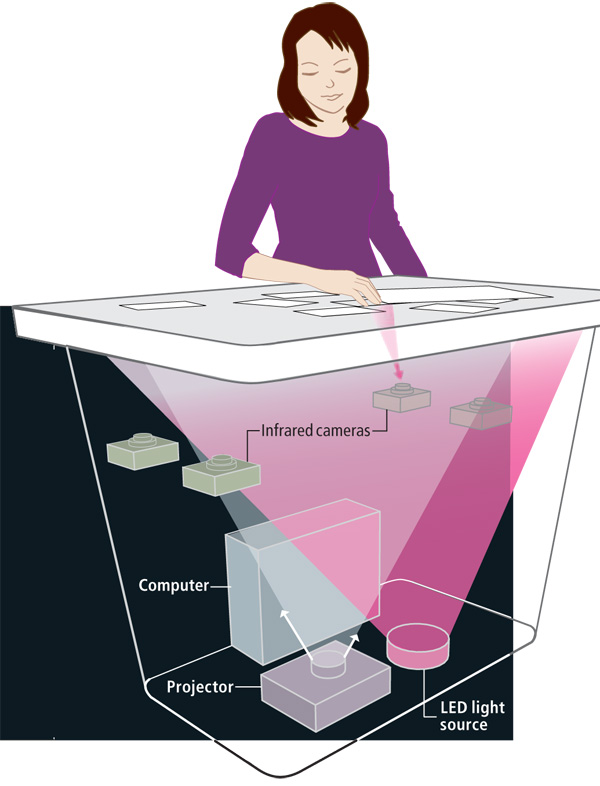
\includegraphics[scale=0.40]{touch_table.jpg}
	\caption{Projeto de mesa multitoque com DI~[\citenum{scient}]}
	\label{touchtable}
	\end{center}
\end{figure}

Como mencionado no cap�tulo anterior, existem dois tipos de ilumina��o principais, \textit{DI}(\textit{Diffuse Illumination}) e \textit{FTIR}(\textit{Frustrated Total Internal Refraction}). A ilumina��o por \textit{DI}, ilustrada na Figura~\ref{touchtable}, consiste de \textit{LED}s que iluminam a mesa por baixo do acr�lico. Esse m�todo � utilizado, por exemplo, na \textit{Microsoft Surface}~[\citenum{microsoftsurface}] e na mesa constru�da para o jogo \textit{Eco-Defense}~[\citenum{pedrosaulo}]. Ao se utilizar este m�todo, tem que se cuidar para que a ilumina��o seja igualmente espalhada pela superf�cie, pois diferen�as de ilumina��o podem dificultar a detec��o de toques corretamente em partes diferentes da mesa. Al�m disto, esta ilumina��o ilumina al�m do toque tudo que est� acima da superf�cie da mesa, possuindo muita interfer�ncia do fundo. Assim, o ambiente no qual se encontra a mesa deve ser controlado para seu correto funcionamento.

O outro m�todo de ilumina��o � o \textit{FTIR}, acompanhado na Figura~\ref{FTIR}. Nesta t�cnica, os LEDS s�o dispostos paralelos ao acr�lico da superf�cie da mesa, ou diretamente dentro do acr�lico atrav�s de furos ao seu redor. Assim, a luz proveniente dos LEDs sofre de um fen�meno denominado reflex�o interna total frustada~[\citenum{TIR}]. Isso significa que a ilumina��o fica retida dentro do acr�lico sem conseguir sair. Ao momento que um dedo toca na superf�cie, a capacidade de refra��o da superf�cie muda, o que permite que a luz saia e ilumine o toque, onde uma c�mera infravermelho consegue captar este dedo, detectando o local do toque. Esse tipo de detec��o � normalmente mais precisa que a detec��o por \textit{DI}, pois sofre menos interfer�ncia do fundo. Entretanto, ela � inadequada no reconhecimento de marcadores fiduciais, pois dependendo do material desses marcadores, n�o h� nitidez na ilumina��o \textit{FTIR} para poder identificar e distinguir as marcas se a superf�cie n�o tiver seu coeficiente de refra��o alterado.

\begin{figure}[h!]
	\begin{center}
	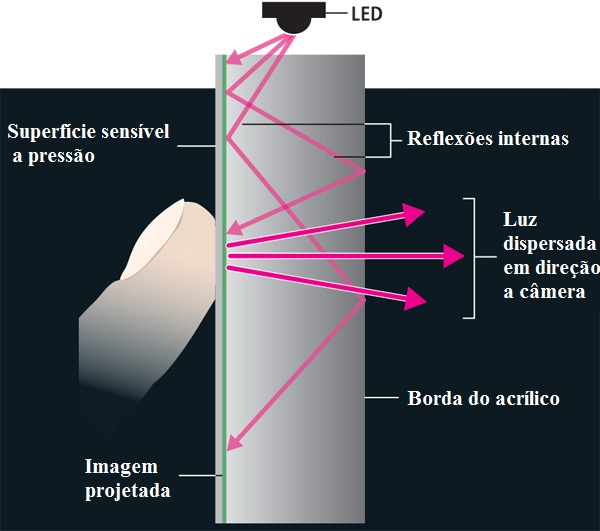
\includegraphics[scale=0.50]{touch_FTIR_port.jpg}
	\caption{Esquema de detec��o de toque FTIR (adaptada de~[\citenum{scient}])}
	\label{FTIR}
	\end{center}
\end{figure}

Outra abordagem trata da combina��o entre as duas abordagens anteriores, exemplificado pela \textit{Virttable}~[\citenum{virttable}] (Figura~\ref{virttable}), que utiliza este m�todo procurando proporcionar a melhor detec��o poss�vel de toques e marcadores fiduciais simultaneamente. Um problema desta abordagem � a interfer�ncia do fundo para a detec��o de toques, fazendo com que o ambiente no qual a mesa se encontra tenha que ser controlado para sua correta detec��o an�logo a ilumina��o DI. No entanto, em rela��o a uma mesa com ilumina��o exclusivamente DI, os toques s�o mais bem iluminados, facilitando as detec��es, o que torna este m�todo mais adequado ao tratamento de fiduciais e toques juntos.

\begin{figure}[h!]
	\begin{center}
	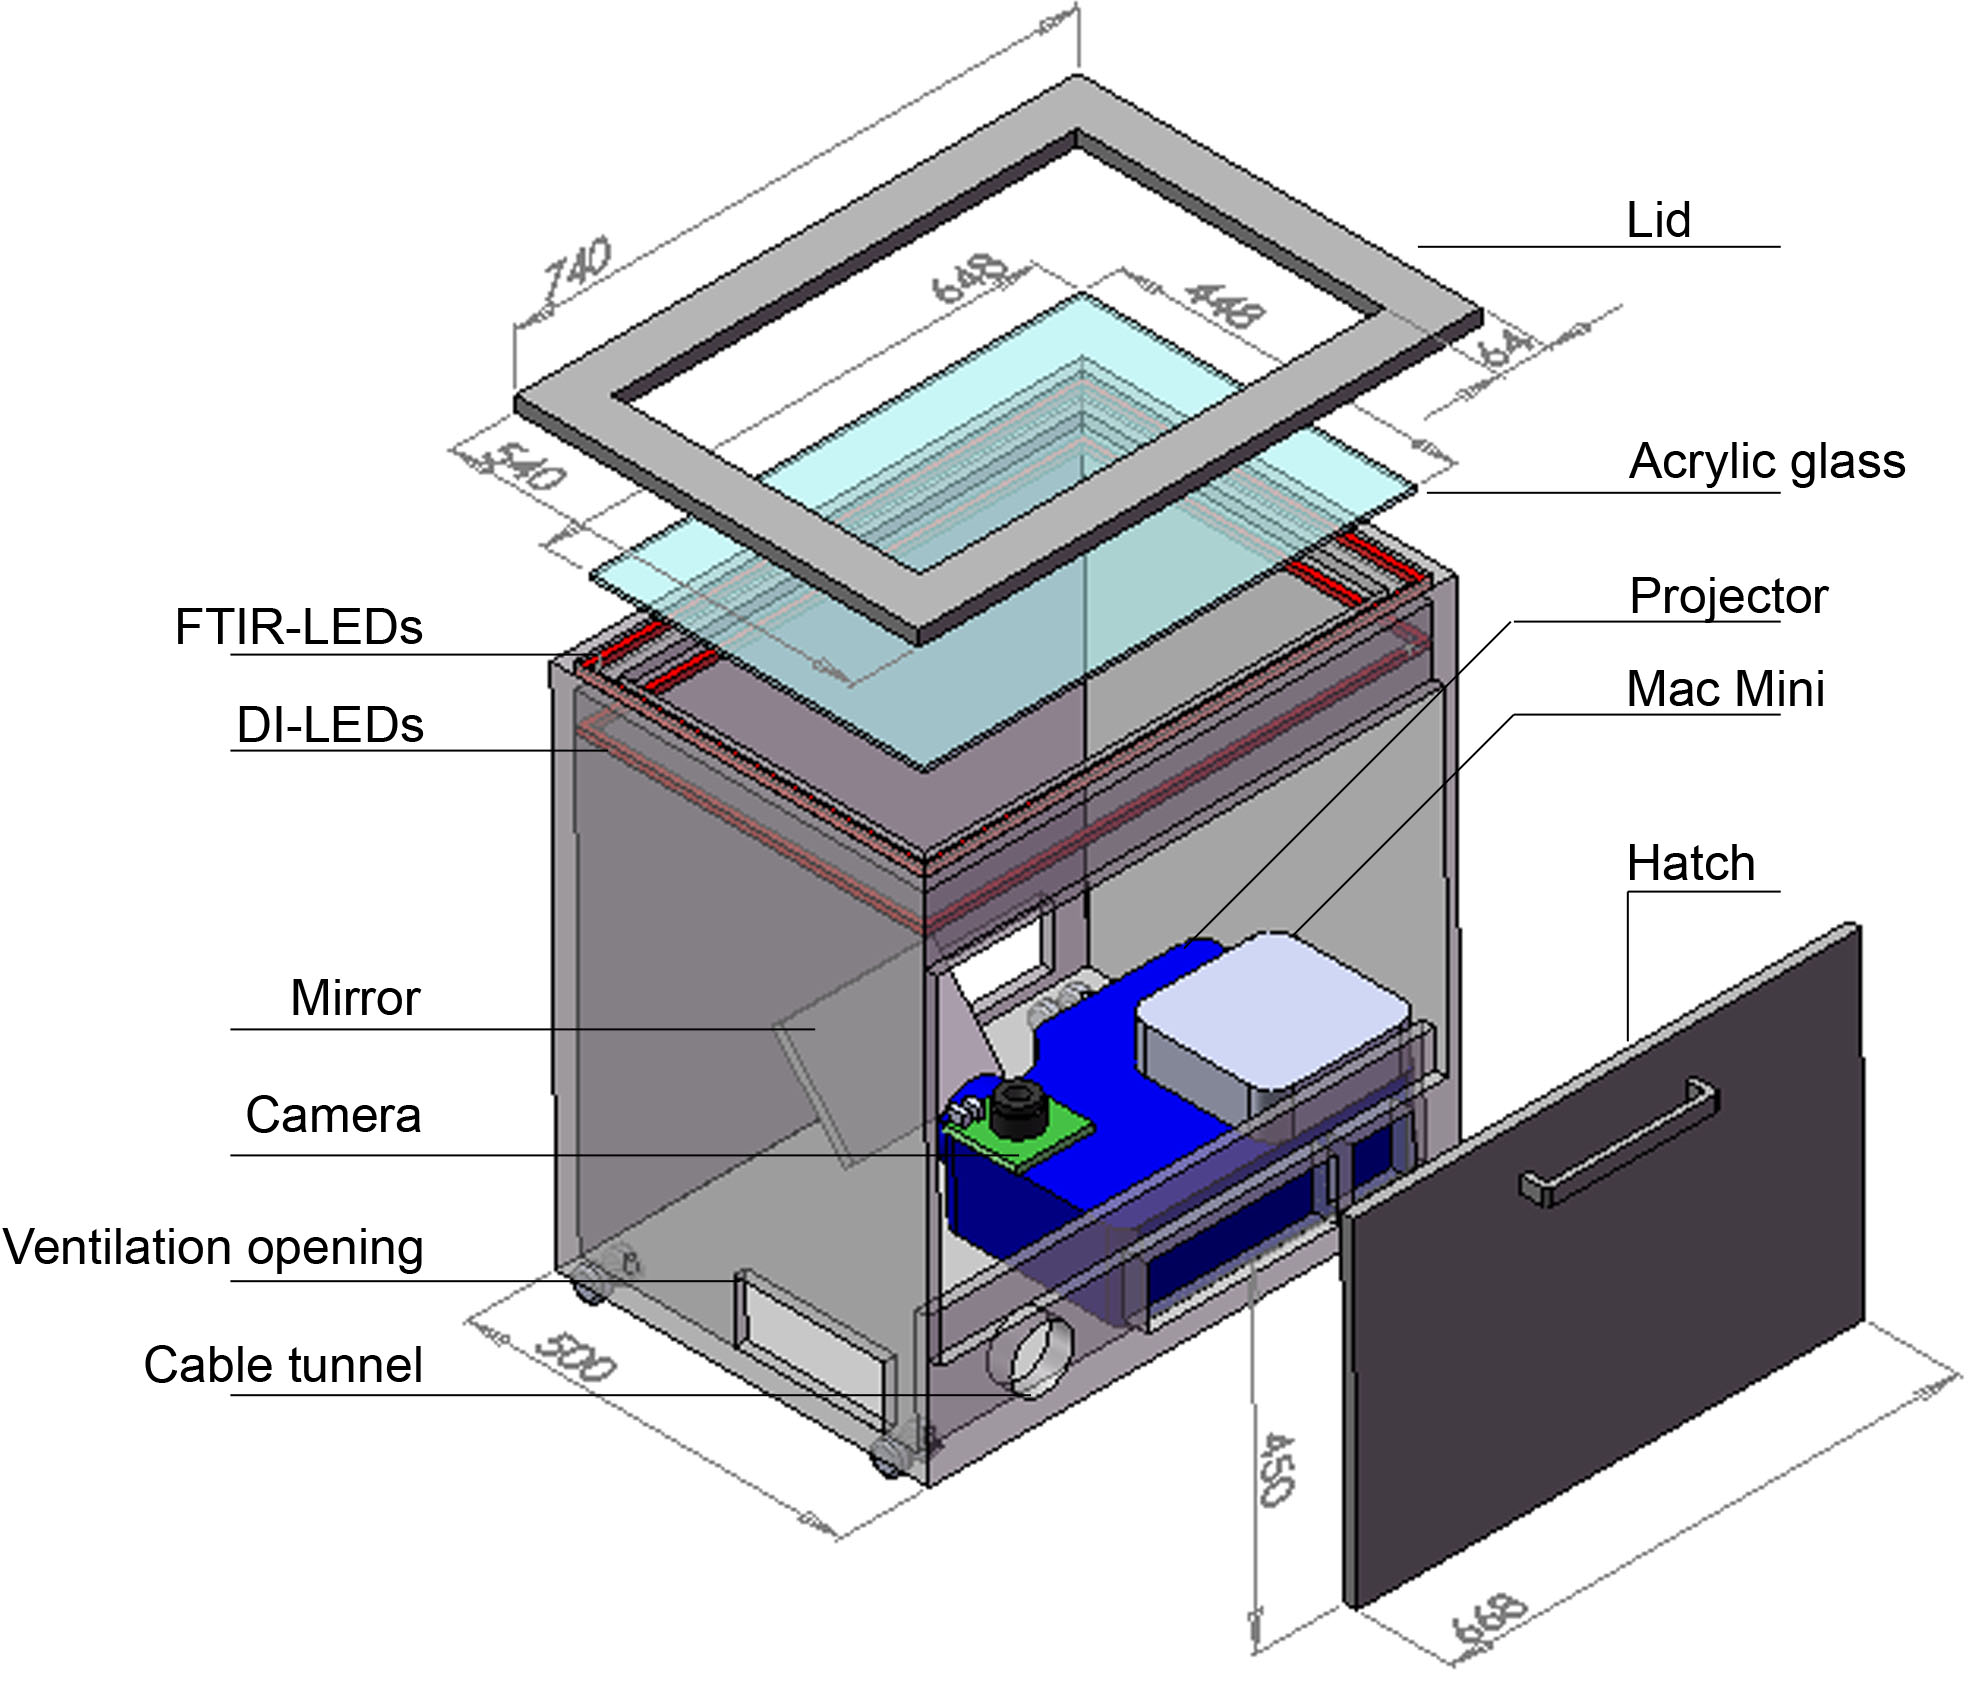
\includegraphics[scale=0.17]{virttable.jpg}
	\caption{Projeto da mesa \textit{Virttable}~[\citenum{virttable}]}
	\label{virttable}
	\end{center}
\end{figure}

\subsection{Processamento das Imagens}
\label{cap3.1.1}

As imagens devem ser capturadas rapidamente em sequ�ncia, de modo que a detec��o de movimento ocorra isenta de erros. A captura dessas imagens se d� por interm�dio de uma c�mera sem filtro infravermelho com um filtro para luz vis�vel, como o negativo de filme fotogr�fico, de forma a simplificar seu formato, facilitando o seu tratamento e evitando que se confundam com as demais imagens de fundo que n�o s�o inerentes ao toque na superf�cie do acr�lico. Depois de capturadas, as imagens s�o filtradas de modo que os toques estejam destacados. Por fim, os conjuntos de \textit{pixels} agrupados que possuem intensidade semelhantes, os chamados \textit{blobs}, s�o detectados e mapeados, demarcando a posi��o exata onde o toque foi realizado.

Conforme mencionado na se��o anterior, existem dois principais m�todos de ilumina��o de uma mesa multitoque, \textit{FTIR}(\textit{Frustrated Total Internal Refraction}) e \textit{DI}(\textit{Diffuse Illumination}). Como � apresentado em~[\citenum{virttable}], a ilumina��o por \textit{FTIR} � mais adequada para detec��o de toques, enquanto a ilumina��o por \textit{DI} � mais indicada para se detectar marcadores fiduciais sobre a mesa. A Figura~\ref{iluminacoes} demonstra as imagens capturadas por uma c�mera localizada dentro da mesa \textit{Virttable} para os diferentes tipos de ilumina��o, ilustrando seu efeito sobre toques e marcadores fiduciais.

\begin{figure}[h!]
	\centering
	\mbox{\subfigure[Sem ilumina��o]{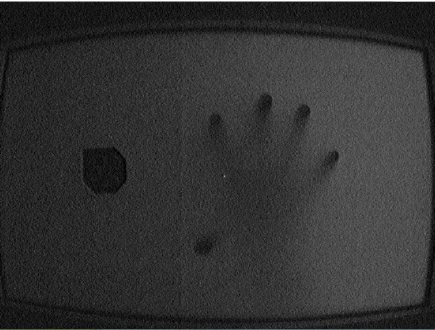
\includegraphics[scale=0.32]{virttableillumination-noillumination.png}}
	\quad
	\subfigure[FTIR]{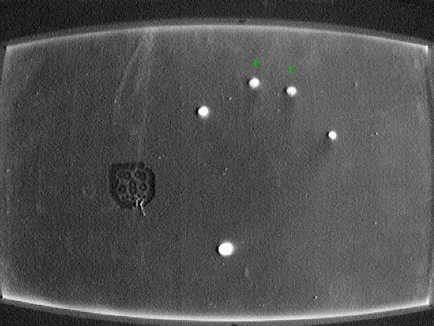
\includegraphics[scale=0.32]{virttableillumination-FTIRonly.png}}
	\subfigure[DI]{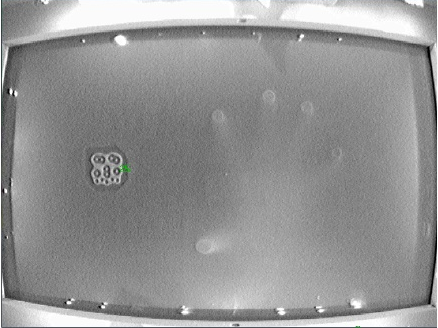
\includegraphics[scale=0.32]{virttableillumination-DIonly.png}}
	\subfigure[FTIR e DI]{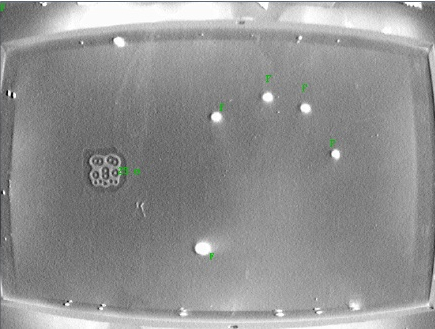
\includegraphics[scale=0.32]{virttableillumination-FTIRandDI.png}}}
	\caption{Imagens capturadas com m�todos de ilumina��o diferentes~[\citenum{virttable}].}
	\label{iluminacoes}
\end{figure}

Dependendo do m�todo de ilumina��o, filtros diferentes devem ser aplicados, como explicado em~[\citenum{muller}], de forma a se excluir interfer�ncias e selecionar apenas os toques. A biblioteca \textit{Community Core Vision}~[\citenum{ccv}], utilizada neste trabalho, possui diversos filtros. Os filtros utilizados ser�o descritos no Cap�tulo~\ref{cap4}.


% Na ilumina��o h�brida, deve-se aplicar todos os filtros correspondentes as duas ilumina��es para obter a melhor imagem poss�vel. Assim, os filtros a serem aplicados s�o apresentados na Figura~[\ref{filtros}]. S�o eles:
%
%
%\begin{figure}[h!]
%	\begin{center}
%	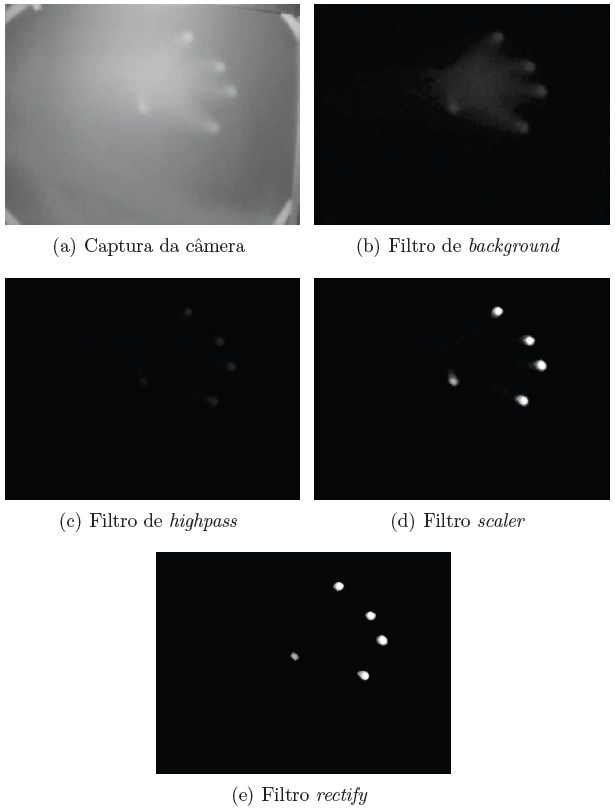
\includegraphics[scale=0.7]{filtros.jpg}
%	\caption{Imagem capturada e suas filtragens~[\citenum{pedrosaulo}].}
%	\label{filtros}
%	\end{center}
%\end{figure} 
%
%\begin{enumerate}
%	\item Imagem capturada do dispositivo (Figura~[\ref{filtros}](a)). Devido a limita��es da biblioteca \textit{Touchlib}, utilizada neste trabalho, ela deve ser composta de um canal de 8-bits, sendo convertida se necess�rio.
%	\item Filtro de \textit{Background} (Figura~[\ref{filtros}](b)), que remove o fundo da imagem, ou seja, aquilo que foi captado e que n�o � o toque do usu�rio ou marcador fiducial e est� a mais na imagem. Para tal, � armazenado um \textit{frame} na mesa sem nada em cima, que ela usa para subtrair dos pr�ximos \textit{frames} esse \textit{frame}, anulando tudo que n�o for modificado da imagem.
%	\item Filtro de \textit{Highpass} (Figura~[\ref{filtros}](c)), que aumenta o brilho de pontos a uma certa altura da mesa. Esse valor � ajustado manualmente pois depende da mesa utilizada, com o prop�sito de atenuar os toques e marcadores fiduciais.
%	\item Filtro \textit{Scaler} (Figura~[\ref{filtros}](d)), que aumenta o brilho da imagem total que restou, clareando mais os toques.
%	\item Filtro \textit{Rectify} (Figura~[\ref{filtros}](e)), que reduz os ru�dos da imagem, deixando os \textit{blobs} mais bem definidos e de f�cil detec��o.
%\end{enumerate}

\subsection{Detec��o de \textit{Blobs}}
\label{cap3.1.2}

Conforme apresentado na se��o anterior, os chamados \textit{blobs}(\textit{Bright Luminescent Objects}) s�o os resultados da detec��o dos toques na superf�cie. Para interpretar esses \textit{blobs}, existem dois processos essenciais, denominados de \textit{Blob-detection}, que interpreta o local em que o \textit{blob} foi criado nas imagens filtradas anteriores, e \textit{Blob-tracking}, que � a an�lise dos \textit{blobs} em uma sequ�ncia de imagens.
Utilizando essas duas an�lises, pode-se identificar a cria��o de \textit{blobs}, verificar seus movimentos durante sua vida �til, e identificar a cria��o de novos \textit{blobs} no sistema. � importante ressaltar que a detec��o de \textit{blobs} deve ser realizada a cada frame.

Ap�s passar pela cadeia de filtros aplicados sobre a imagem da c�mera,  ela alcan�a seu est�gio final aonde s�o destacadas as intera��es com a interface. A partir dessa imagem final � observado os contornos dos \textit{blobs} que aparecem e s�o analisados para identificar se eles correspondem ao toque de dedos ou a marcadores fiduciais. Se for um toque, uma elipse � feita sobre ele, e com base nela, pode ser identificada a posi��o, orienta��o e tamanho do \textit{blob}. Esse \textit{blob} ent�o � adicionado a uma lista para ser processado.

Com base nessa lista, o \textit{blob-tracking} tem que ser feito para identificar a movimenta��o e cria��o dos \textit{blobs}. Usando o frame anterior de refer�ncia, verifica-se se o \textit{blob} foi criado, removido ou atualizado. Para se fazer essa an�lise, s�o utilizados dois conjuntos: \textit{P} e \textit{Q}. O conjunto \textit{P} cont�m a lista de pontos que representam os \textit{blobs} do frame anterior. Como exemplo, apresenta-se um conjunto \textit{P} com pontos (1,1) e (4,4), ilustrado no gr�fico da Figura~\ref{grafP}.

\begin{figure}[h!]
	\begin{center}
	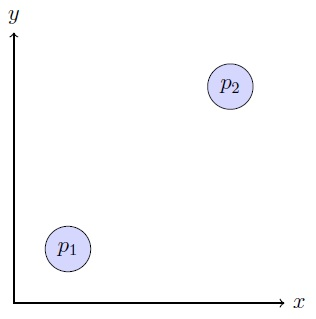
\includegraphics[scale=1]{GraficoP.jpg}
	\caption{Gr�fico de P~[\citenum{pedrosaulo}].}
	\label{grafP}
	\end{center}
\end{figure} 

O segundo conjunto, \textit{Q}, cont�m a lista de pontos que comp�e os \textit{blobs} do frame atual. O gr�fico da Figura~\ref{grafQ} apresenta um exemplo para o conjunto Q com pontos (1,2), (1,4) e (4,3).

\begin{figure}[h!]
	\begin{center}
	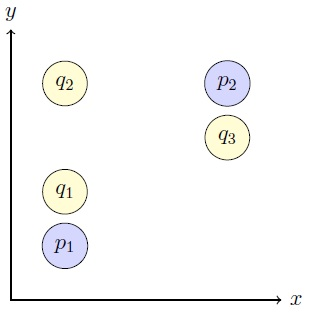
\includegraphics[scale=1]{GraficoQ.jpg}
	\caption{Gr�fico de Q~[\citenum{pedrosaulo}].}
	\label{grafQ}
	\end{center}
\end{figure} 

O n�mero de elementos de \textit{Q} � maior que o n�mero de elementos em \textit{P}, logo, pelo menos um \textit{blob} novo foi criado. Para saber qual o \textit{blob} foi criado e quais foram somente atualizados, deve-se analisar as dist�ncias entre os \textit{blobs}. Neste exemplo � demonstrado que o \textit{blob} \textit{p1} se moveu para \textit{q1}, o \textit{blob} \textit{p2} se moveu para \textit{q3}, e o \textit{q2} � um novo \textit{blob} criado neste frame. A cada frame, esse conjunto \textit{Q} passa a ser o novo \textit{P}, um novo conjunto \textit{Q} � gerado, e o procedimento se repete.

\subsection{Corre��o da c�mera}
\label{cap3.1.3}

Quando uma c�mera captura uma imagem sobre uma superf�cie plana, essa imagem possui uma distor��o, onde os pontos mais distantes do centro da imagem ganham um pequeno �ngulo em rela��o � imagem original, pois s�o exibidos de forma reduzida. Ao se detectar \textit{blobs}, � necess�rio executar alguns algoritmos a fim de corrigir essa distor��o e colocar a imagem inteira em um mesmo plano. De acordo com \textit{Muller} em~[\citenum{muller}], v�rias bibliotecas de processamento de imagem e detec��o de multitoque j� fazem isso. Na Figura~\ref{distorcao} � poss�vel visualizar uma imagem antes e depois da corre��o.

\begin{figure}[h!]
\centering
\mbox{\subfigure[Imagem da c�mera com distor��o.]{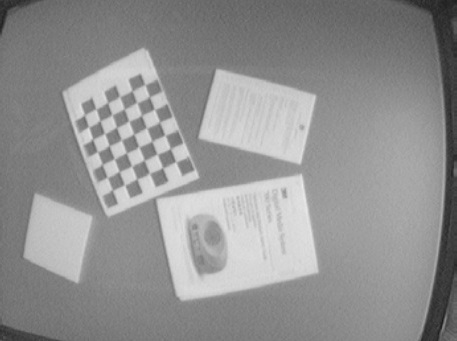
\includegraphics[scale=0.5]{distorcao(a).jpg}}
\quad
\subfigure[Imagem da c�mera corrigida.]{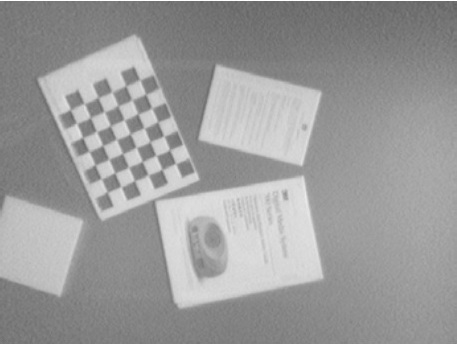
\includegraphics[scale=0.5]{distorcao(b).jpg}}}
\caption{Corre��o da distor��o focal da c�mera~[\citenum{muller}].}
\label{distorcao}
\end{figure}

Segundo \textit{Muller}~[\citenum{muller}], essa corre��o realiza um mapeamento de pontos na imagem em rela��o a um ponto do espa�o. Para tal, � necess�rio considerar a dist�ncia focal, o centro da imagem, o tamanho de cada pixel, o coeficiente de distor��o radial da lente, as propriedades da pr�pria c�mera, bem como o vetor de transla��o e a matriz de rota��o que analisam o espa�o em que se encontra a c�mera.

Assim, um ponto na c�mera pode ser corrigido de acordo com a equa��o \begin{equation}m = A[Rt]M\label{eq:correcaodistorcao}\end{equation} onde \textit{A} � a matriz que possui os fatores da c�mera (Equa��o~\ref{eq:matrizA}), \textit{M} � um ponto do espa�o, \textit{R} � a matriz de rota��o da c�mera e \textit{t} � o vetor de transla��o da mesma.

\begin{equation}
	A =
	\begin{vmatrix}
	  f_{x}   &	0		& c_{x}	\\ 
	  0			& f_{x}	&	0		\\
	  0			&	0		&	1
	\end{vmatrix}
	\label{eq:matrizA}
\end{equation}

Equa��o dos fatores da c�mera, onde f\textsubscript{x},f\textsubscript{y} e c\textsubscript{x},c\textsubscript{y} correspondem, respectivamente, a dist�ncia focal e o centro da c�mera em um ponto (x,y) arbitr�rio da imagem.

Essas medi��es podem ser realizadas analizando uma imagem com um padr�o reconhecido sendo colocada em pontos diferentes da c�mera. Ao se processar esta imagem, pode-se medir a diferen�a entre o seu tamanho ideal e o tamanho obtido para se obter os valores ditos antes. Por�m, filtros que aplicam esta corre��o podem ser pesados, deixando mais lenta a captura de toques.

Uma alternativa a esta corre��o seria a adapta��o de toques, como � feito pela \textit{CCV} (\textit{Community Core Vision}). Neste caso, s�o desenhados pontos na superf�cie em que o usu�rio deve tocar quando requisitado, como pode ser observado na Figura~\ref{calibrando}. Assim, o programa grava a posi��o em que o toque foi realizado, e ao se realizar um toque futuramente, sua posi��o � recalculada imediatamente baseada na proximidade com os pontos obtidos na calibra��o. Esta forma � mais eficiente que a aplica��o do filtro de \textit{barrel correction}, e possui uma precis�o boa dependendo de quantos pontos forem usados na calibra��o.

\begin{figure}[h!]
	\begin{center}
	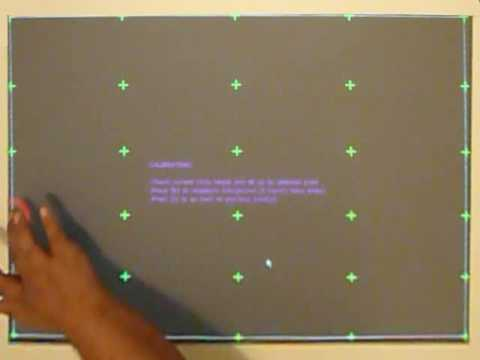
\includegraphics[scale=0.5]{calibrando.jpg}
	\caption{Calibra��o de pontos na \textit{CCV}~[\citenum{calibrando}].}
	\label{calibrando}
	\end{center}
\end{figure} 

\section{Aspectos de mesas com superf�cie multitoque}
\label{cap3.2}

As mesas com superf�cies multitoque mudam a forma como o usu�rio interage com o computador. Devido a esse novo paradigma, � necess�rio repensar as capacidades que elas oferecem aos usu�rios. Os \textit{softwares} atuais levam em considera��o que o usu�rio esta sentado na frente de uma tela, controlando um dispositivo apontador, o \textit{mouse}. Uma mesa multitoque, no entanto, convida v�rias pessoas a partilharem simultaneamente a sua utiliza��o. Neste contexto, observa-se que a maioria dos \textit{softwares} atuais n�o est�o aptos a serem utilizados neste tipo de estrutura de interface, pois n�o possuem suporte a toques m�ltiplos e simult�neos.

Al�m disso, para que as mesas tornem-se comum no dia-a-dia das pessoas, elas devem ter um desempenho eficiente compat�vel com a realidade dos usu�rios. Nesta se��o � discutido quest�es referentes ao n�mero de usu�rios, o n�mero de toques, os tipos de toque, a resolu��o e o tamanho da mesa.

\subsection{Tamanho e Resolu��o}
\label{cap3.2.1}

O tamanho de uma mesa multitoque deve ser proporcional a sua utiliza��o. Se for projetada para ser utilizada por poucos usu�rios, deve ter um tamanho que permita para que um �nico usu�rio alcance todos seus lados. No entanto, se a mesa for dimensionada para o uso em grupo de um n�mero indeterminado de usu�rios, pode ter seu tamanho aumentado at� os limites impostos pela proje��o da imagem sob o acr�lico, realizada pelo projetor multim�dia, e pelo �ngulo de abertura da c�mera utilizada para identificar os toques.

Idealmente, os \textit{softwares} devem funcionar independentemente do tamanho da mesa, permitindo que o mesmo seja utilizado em projetos similares. No entanto, mesmo sem este planejamento, existem maneiras de tratar isso. A mesa pode ser projetada para se utilizar um dispositivo apontador, permitindo a um usu�rio alcan�ar pontos mais distantes, ou ent�o possuir uma fun��o que mude o tamanho da tela e a posicione mais perto do usu�rio.

Em geral, as mesas possuem um tamanho maior que os monitores de v�deo tradicionais, o que produz um problema sobre a resolu��o da imagem projetada. A maioria dos projetores possuem resolu��o padr�o de 800x600 ou 1024x768 pixels, o que, para mesas grandes, � insuficiente e produz uma imagem distorcida. Para contornar isso, a solu��o � utilizar um projetor \textit{short-throw} de alta resolu��o \textit{WXGA (Wide eXtended Graphics Array)}, capaz de atingir qualidade de imagem projetada em alta defini��o como o \textit{720p}(resolu��o 1280x720 com varredura progressiva~\ref{}) ou at� o \textit{1080p}(resolu��o 1650x1080 com varredura progressiva~\ref{}). Projetores \textit{short-throw} s�o capazes de projetarem imagens maiores em rela��o a sua dist�ncia da superf�cie de proje��o, quando comparados a projetores convencionais.

\subsection{Interfaces}
\label{cap3.2.2}

Como citado por Brand�o et al.~[\citenum{pedrosaulo}], interfaces sens�veis ao toque trazem ao usu�rio a possibilidade de interagir diretamente com os dados. Isso conduz um grande apelo ao usu�rio, pois al�m de ser natural, � de f�cil aprendizado. Por n�o possuir partes m�veis, as interface sens�veis ao toque tamb�m podem ser usadas em equipamentos acess�veis ao p�blico, tais como caixas autom�ticos e pontos de acesso a servi�os espec�ficos.

Como mencionado no in�cio deste cap�tulo, a maioria \textit{softwares} existentes s�o desenvolvidos para utiliza��o por meio de teclado e \textit{mouse}. No caso do \textit{mouse}, a �rea apontada pelo cursor � bem pequena, logo, as interfaces possuem poucos p�xeis para a sele��o. No entanto, em interfaces sens�veis ao toque h� uma configura��o diferente, pois o dedo humano � maior que o ponteiro do um \textit{mouse}, podendo acarretar em perda de precis�o na detec��o do local do toque. Segundo Brand�o et al.~[\citenum{pedrosaulo}], a qualidade da c�mera � um fator determinante na precis�o da interface, pois como ela captura a imagem a ser processada, diversos aspectos como luz, dist�ncia focal e resolu��o alteram a imagem capturada afetando a usabilidade para o usu�rio.
Isto porque, em imagens muito claras � dif�cil identificar corretamente os \textit{blobs}, sendo assim, a c�mera deve possuir um filtro de luz. A dist�ncia focal da c�mera deve suportar a dist�ncia entre a superf�cie da mesa e a c�mera para que a imagem n�o seja capturada sem foco. Al�m disso, a c�mera deve possuir uma boa resolu��o para capturar imagens com melhor qualidade.

� fundamental salientar que o aumento da resolu��o resulta em uma amostragem de \textit{pixels} mais alta em cada imagem, o que auxilia nas dificuldades relativas � precis�o da c�mera, pois permite que as capturas apresentem com mais fidelidade o local dos \textit{blob}s. Contudo, a quest�o do tamanho do toque deve ser considerada durante a constru��o da interface, pois este pode ser maior que o bot�o desejado e abranger uma regi�o maior que a esperada. Em geral, o ponto tomado como refer�ncia da posi��o do toque � o seu ponto central.

Al�m desses problemas, existe a quest�o do ponto de vis�o do usu�rio. Quando um usu�rio utiliza um computador, ele est� acostumado a possuir uma interface virada para ele. No caso da mesa, h� v�rios usu�rios e eles podem estar olhando a mesa de �ngulos diferentes. A interface deve ser agrad�vel para todos os usu�rios que forem utilizar a mesa. A diferen�a de �ngulo de vis�es � melhor exemplificado na Figura~\ref{OK}.

\begin{figure}[h!]
	\begin{center}
	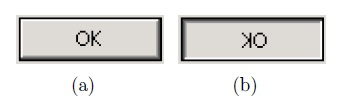
\includegraphics[scale=0.8]{ok.jpg}
	\caption{O tradicional bot�o \textit{OK} visto por dois �ngulos distintos~[\citenum{pedrosaulo}].}
	\label{OK}
	\end{center}
\end{figure}

Assim, ao se planejar um software para uma mesa multitoque, deve-se prever a rota��o da interface de modo a acomodar a aplica��o de acordo com a posi��o do(s) usu�rio(s).

\subsection{N�mero de Usu�rios}
\label{cap3.2.3}

Neste contexto de mesas multitoque, uma das principais dificuldades com rela��o ao n�mero indeterminado de usu�rios, � identificar a quem pertence determinado toque, bem como atribuir as propriedades necess�rias a cada um deles. Toma-se o exemplo usado em~[\citenum{pedrosaulo}], que cita o caso de uma aplica��o para desenho em que um usu�rio deseja trocar a cor de seu pincel, de amarelo para azul, acarretando em um problema na decis�o de trocar a cor para somente o usu�rio desejado.

A solu��o, nesse caso, � trocar a cor para todos os toques, ou ent�o implementar a divis�o de �reas de trabalho, onde cada usu�rio possui sua respectiva �rea e as modifica��es feitas em sua �rea n�o afetam as de outros usu�rios.

\subsection{Detec��o de Gestos}
\label{cap3.2.4}

A maioria dos \textit{softwares} leva em considera��o que os gestos s�o oriundos apenas de um �nico \textit{input}, o \textit{mouse}. Assim, s�o implementados geralmente gestos com um ponto de contato. Tradicionalmente, existem o seguintes gestos:

\begin{itemize}
	\item{\textit{Click} (Figura~\ref{ClickDrag}(a))}: gesto mais simples e tradicional. � detectado ao se estabelecer um ponto de contato que � retirado logo em seguida.
	
	\begin{figure}[h!]
	\centering
	\mbox{\subfigure[\textit{Click}]{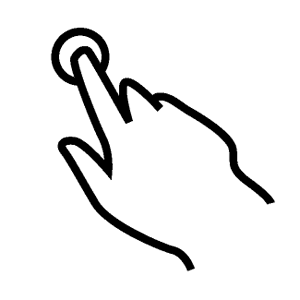
\includegraphics[scale=0.5]{click.png}}
	\quad
	\subfigure[\textit{Drag}]{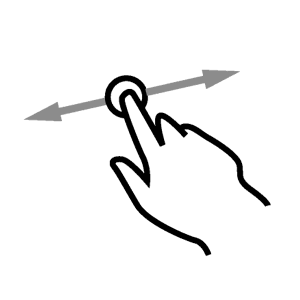
\includegraphics[scale=0.5]{drag.png}}}
	\caption{Gestos de \textit{Click} e \textit{Drag}~[\citenum{gestos}].}
	\label{ClickDrag}
	\end{figure}
		
	\item{\textit{Drag} (Figura~\ref{ClickDrag}(b))}: continua��o do gesto acima (Click), identificado ao se estabelecer um ponto de contato seguido de movimenta��o antes da retirada do contato.
	
\end{itemize}

Poucos \textit{softwares} implementam algum tipo de gesto diferente usando somente um ponto de contato compostos de desenhos, como o que ocorre no jogo \textit{Black and White}~[\citenum{blackandwhite}] em que o jogador pode selecionar um poder diferente dependendo do movimento que faz com o mouse, ilustrado na Figura~\ref{blackwhite}.

\begin{figure}[h!]
	\begin{center}
	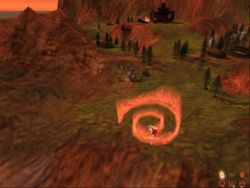
\includegraphics[scale=1.5]{blackwhite.jpg}
	\caption{Reconhecimento de gesto no jogo \textit{Black and White}~[\citenum{blackandwhite}].}
	\label{blackwhite}
	\end{center}
\end{figure}

Para identificar esse tipo de gesto � preciso identificar a forma que o usu�rio est� desenhando na tela. Isso � feito a partir da identifica��o da dire��o em que o jogador est� desenhando e o �ngulo que ele est� seguindo. Como o ser humano n�o possui uma precis�o exata para desenhar, esses valores t�m que ser aproximados e comparados a um banco de dados de gestos conhecidos, e aquele que se aproximar mais do padr�o, dentro de um limite, � o gesto detectado. Caso n�o se aproxime de nenhum gesto conhecido, o gesto n�o � reconhecido e o usu�rio deve fazer outro gesto. 

Em uma mesa multitoque a possibilidade de identifica��o de v�rios pontos de contato habilita a implementa��o de outros gestos, al�m dos mencionado acima. Como exemplo, podemos citar:

\begin{itemize}
	\item{\textit{Rotate} (Figura~\ref{rotateScale}(a))}: dois pontos de contato s�o inseridos sobre uma superf�cie e s�o movimentados em dire��es opostas, enquanto se mant�m a dist�ncia entre os dois dedos constantes. O �ngulo entre os dois dedos � calculado e denomina a rota��o do objeto.
	
	\begin{figure}[h!]
	\centering
	\mbox{\subfigure[\textit{Rotate}]{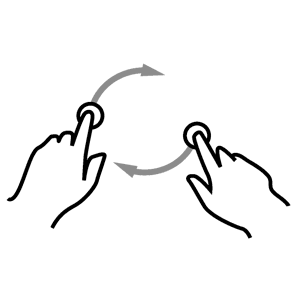
\includegraphics[scale=0.5]{rotate.png}}
	\quad
	\subfigure[\textit{Scale}]{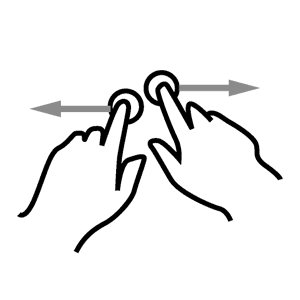
\includegraphics[scale=0.5]{scale.png}}}
	\caption{Gestos de \textit{Rotate} e \textit{Scale}~[\citenum{gestos}].}
	\label{rotateScale}
	\end{figure}
		
	\item{\textit{Scale} (Figura~\ref{rotateScale}(b))}: an�logo ao \textit{Rotate}, utiliza dois pontos de contato sobre uma superf�cie, por�m, neste caso mant�m-se o �ngulo constante e varia-se a dist�ncia entre os dedos. Uma diminui��o na dist�ncia significa uma diminui��o na escala, enquanto um aumento de dist�ncia significa um aumento de escala.
		
\end{itemize}

Al�m destes, podem existir v�rios gestos n�o tradicionais, como m�ltiplos pontos de contato seguindo em dire��es diferentes para selecionar uma op��o, por exemplo, como pode ser observado em~[\citenum{touchmenu}]. Analisando a quantia de pontos poss�veis em uma mesa, existem in�meras possibilidades de gestos usando combina��es de pontos de contato.

\chapter{Constru��o da Mesa Multi-toque}
\label{cap4}
Este cap�tulo apresenta o projeto, a constru��o e a montagem da mesa multi-toque concebida como plataforma de execu��o do \textit{software Deskworld} proposto neste trabalho. Para ilumina��o da superf�cie da mesa e reconhecimento dos toques utilizou-se o m�todo \textit{FTIR}.

\section{Estrutura da Mesa}
\label{cap4.1}

\begin{figure}[h!]
	\begin{center}
	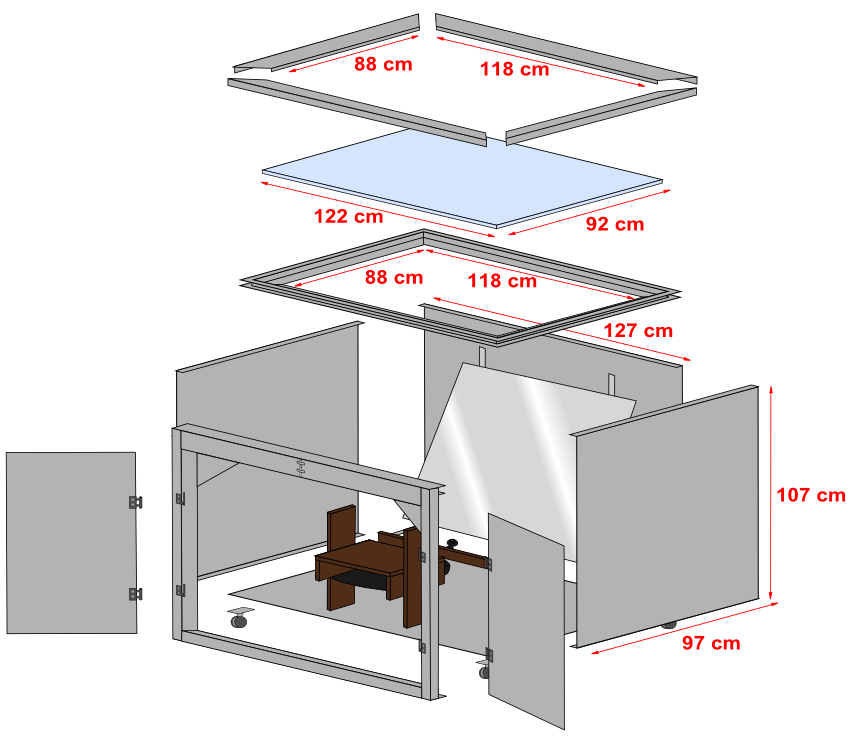
\includegraphics[scale=0.6]{projetomesa.png}
	\caption{Projeto da mesa com superf�cie multi-toque constru�da neste trabalho.}
	\label{mesa}
	\end{center}
\end{figure}

\begin{figure}[h!]
	\begin{center}
	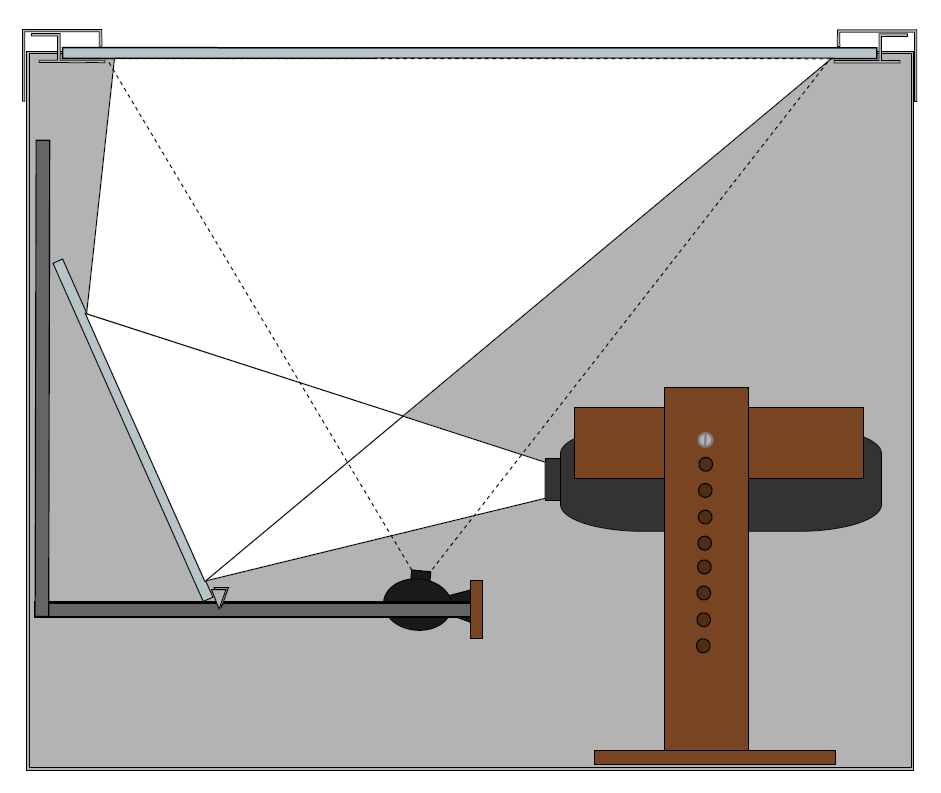
\includegraphics[scale=0.6]{mesalateral.png}
	\caption{Vis�o lateral do projeto da mesa com superf�cie multi-toque constru�da neste trabalho.}
	\label{mesalateral}
	\end{center}
\end{figure}

A estrutura da mesa � feita de alum�nio como material principal, de modo a prover estabilidade, leveza e mobilidade, sem prejudicar sua efici�ncia. Sua confec��o foi sob medida, pois cada elemento influi na sua configura��o. As dimens�es da mesa est�o inclusas na Figura~\ref{mesa} que apresenta o projeto da mesa. Vis�o de dentro e lateral do projeto da mesa est� ilustrada na Figura~\ref{mesalateral}.

Outra caracter�stica importante da mesa � a possibilidade de ser desmontada, o que facilita seu transporte. Apesar de possuir grandes medidas, uma vez desmontada pode ser facilmente carregada e armazenada, pois sua estrutura de alum�nio � leve. Al�m disso, mesmo montada, a mesa possui rodas com travas para facilitar a movimenta��o, podendo ser travada no local de uso. A mesa completa pode ser observada, externa e internamente, nas Figuras~\ref{mesaporfora} e~\ref{mesadentro}, respectivamente.

\begin{figure}[h!]
	\centering
	\mbox{\subfigure{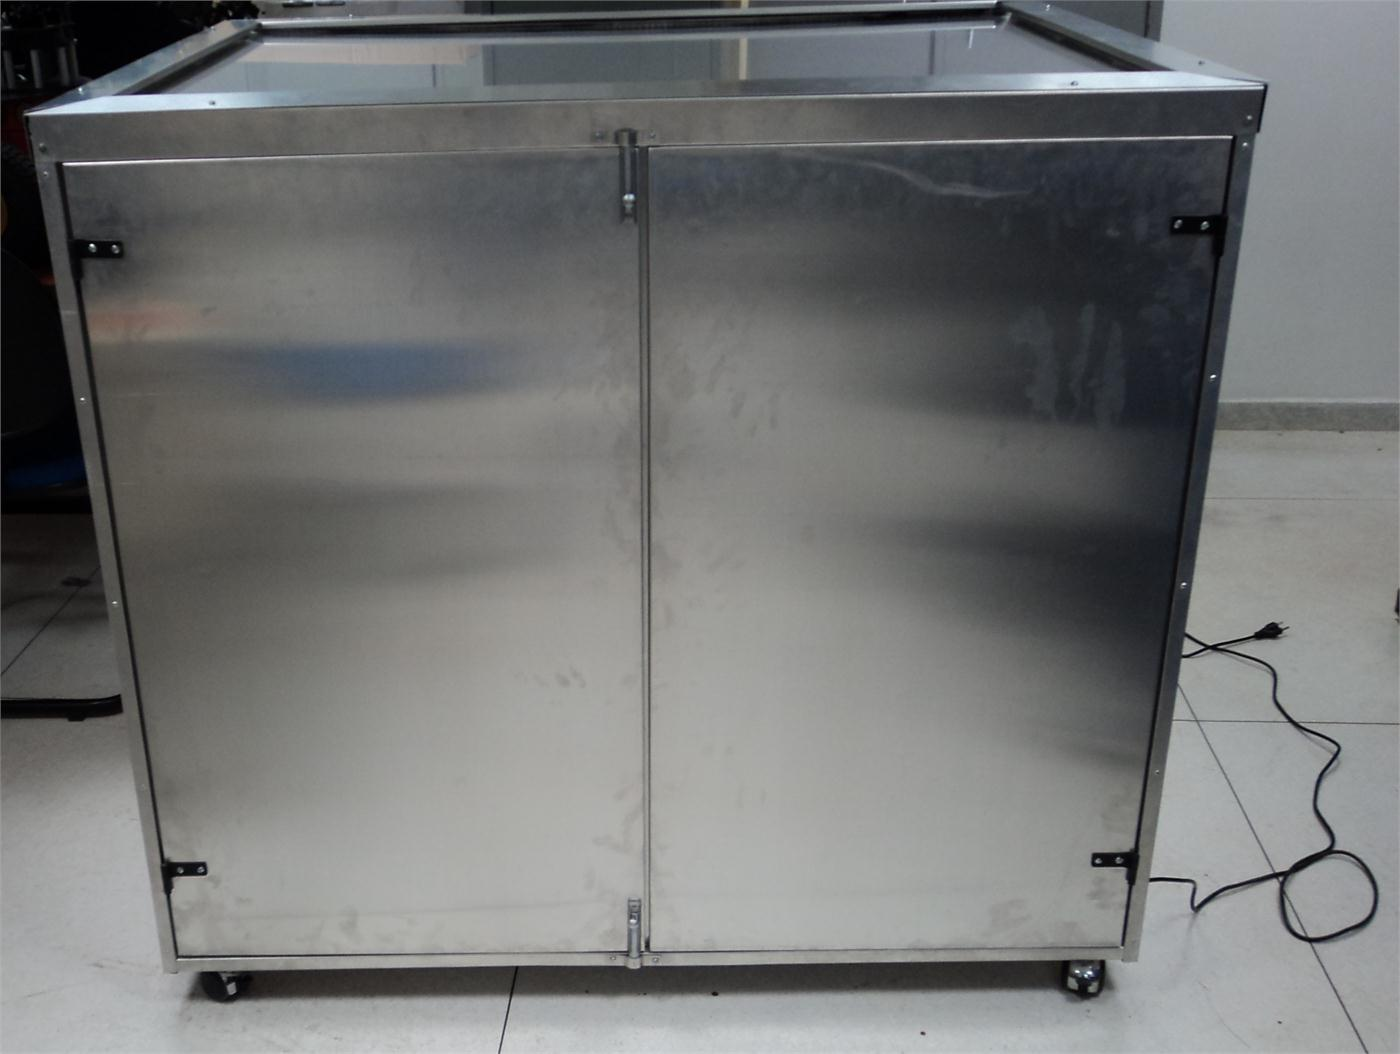
\includegraphics[scale=0.18]{mesapaisagem.jpg}}}
	\mbox{\subfigure{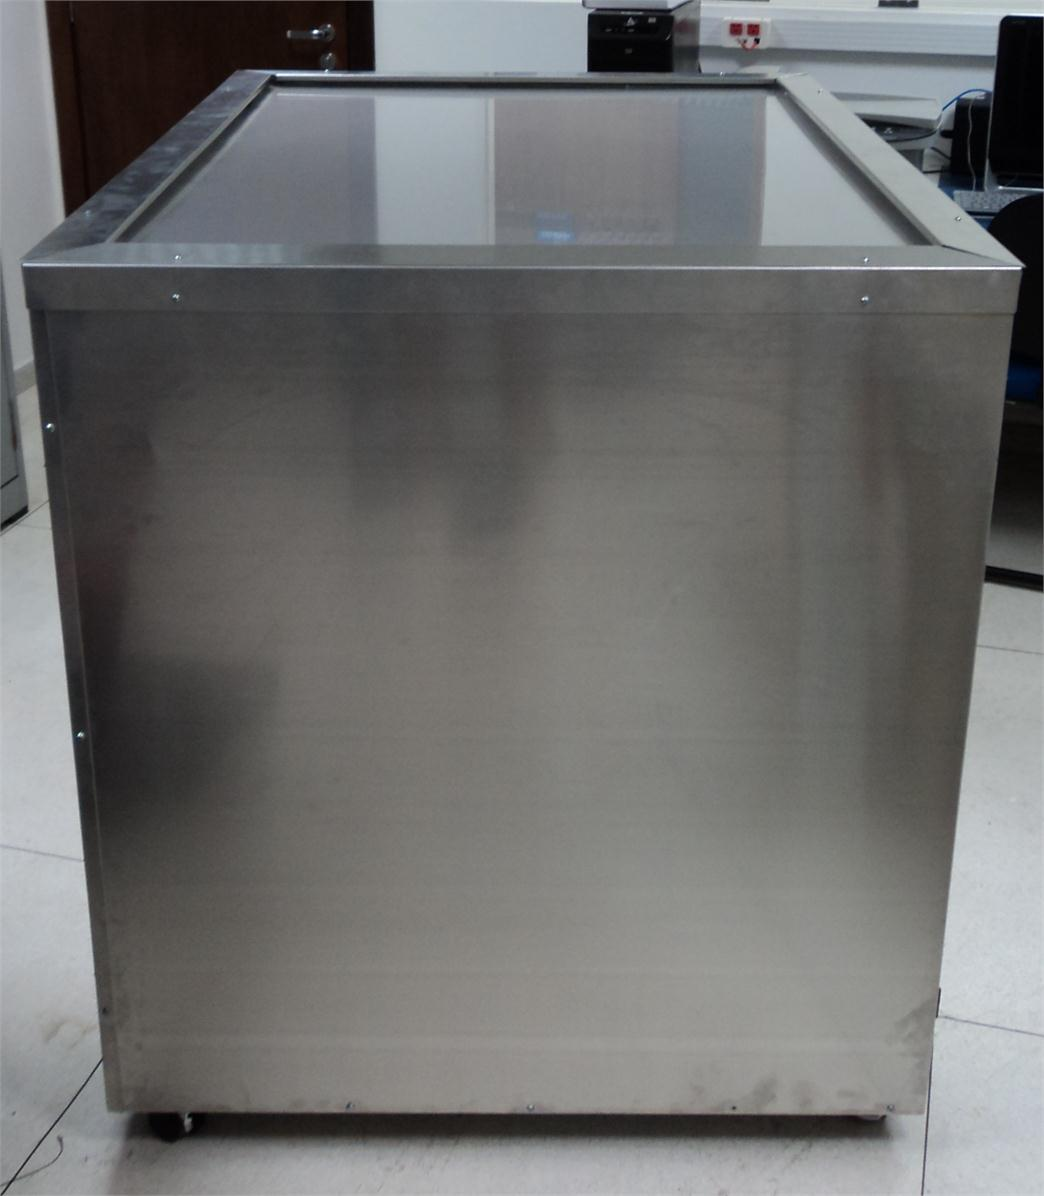
\includegraphics[scale=0.1]{mesaretrato.jpg}}
	\quad
	\subfigure{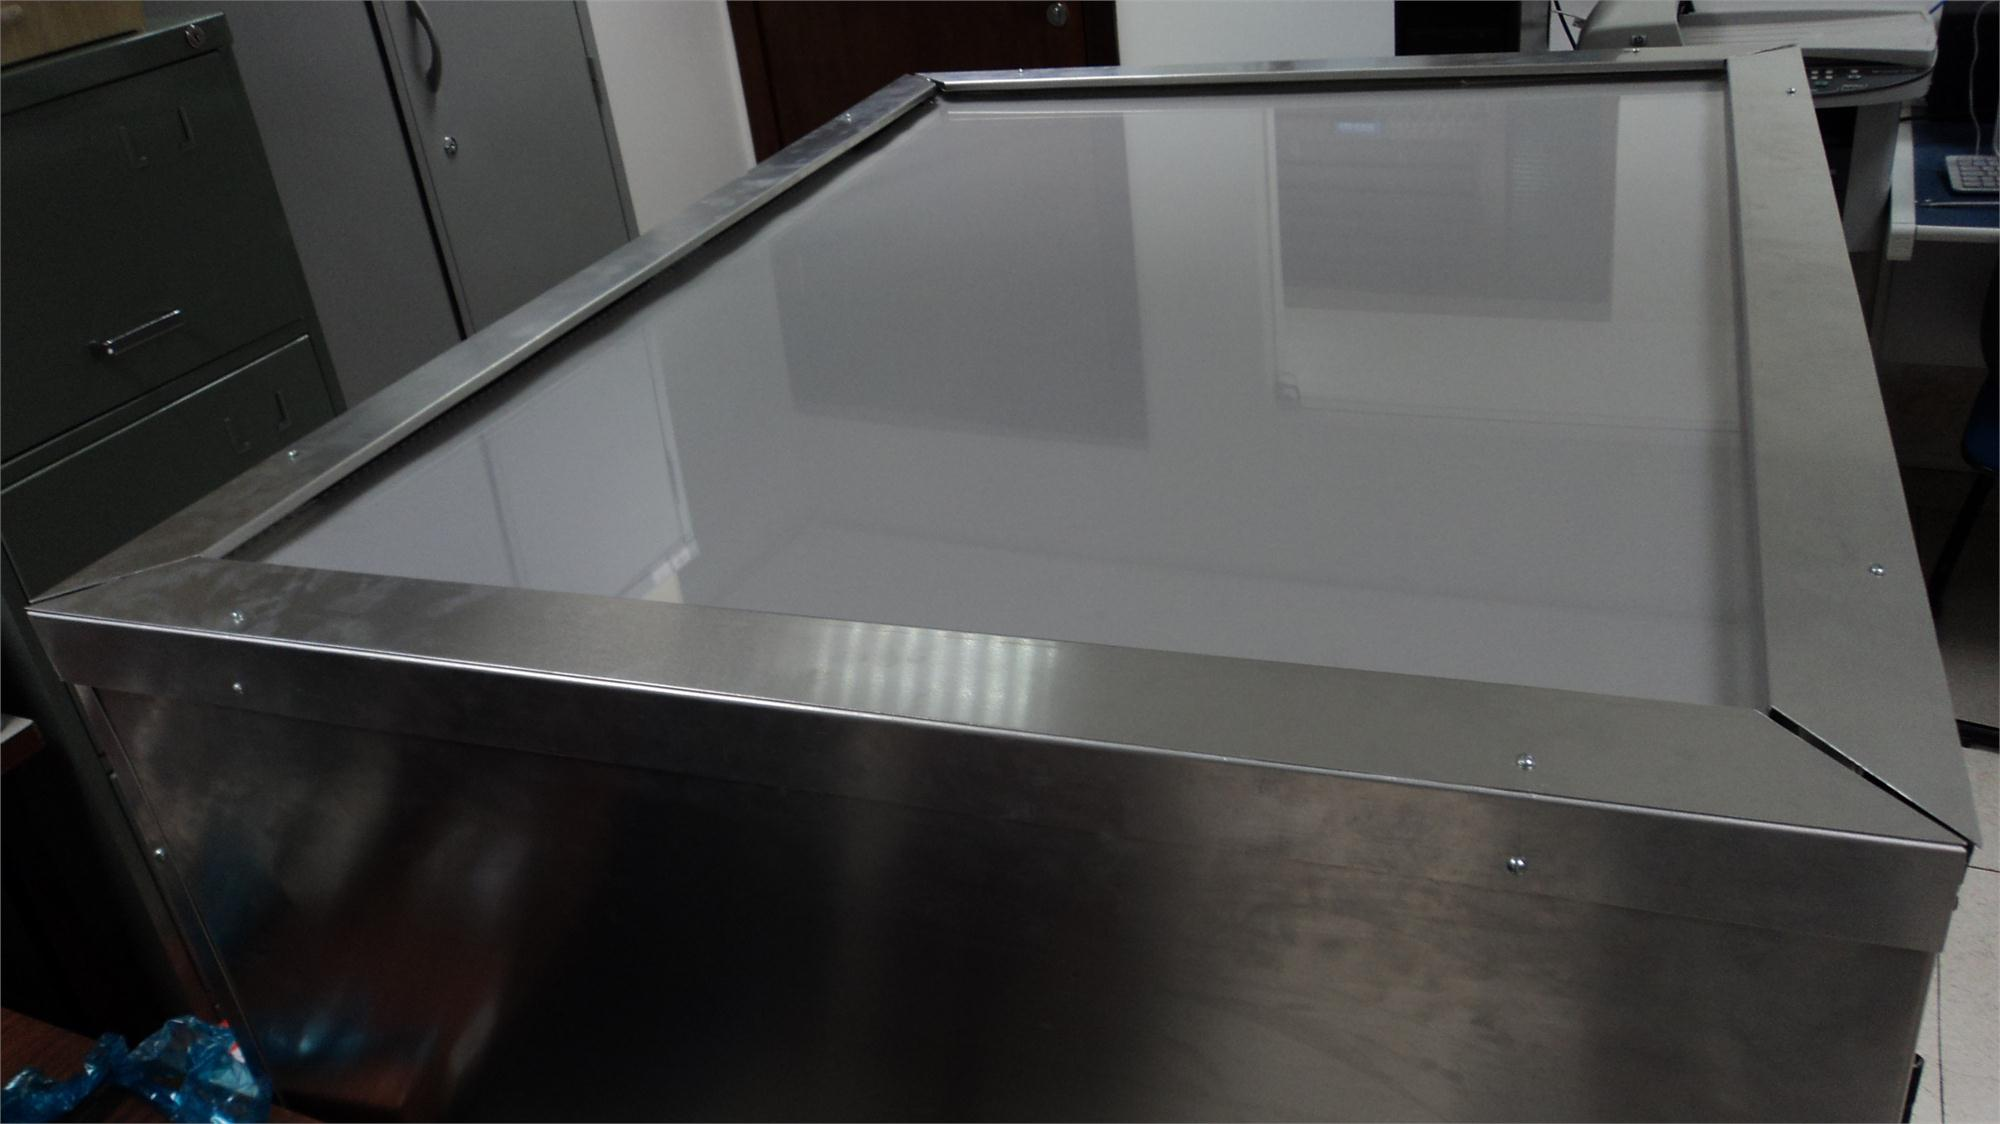
\includegraphics[scale=0.05]{mesaporfora.jpg}}}
	\caption{Fotos da mesa multi-toque constru�da neste projeto.}
	\label{mesaporfora}
\end{figure}

\begin{figure}[h!]
	\begin{center}
	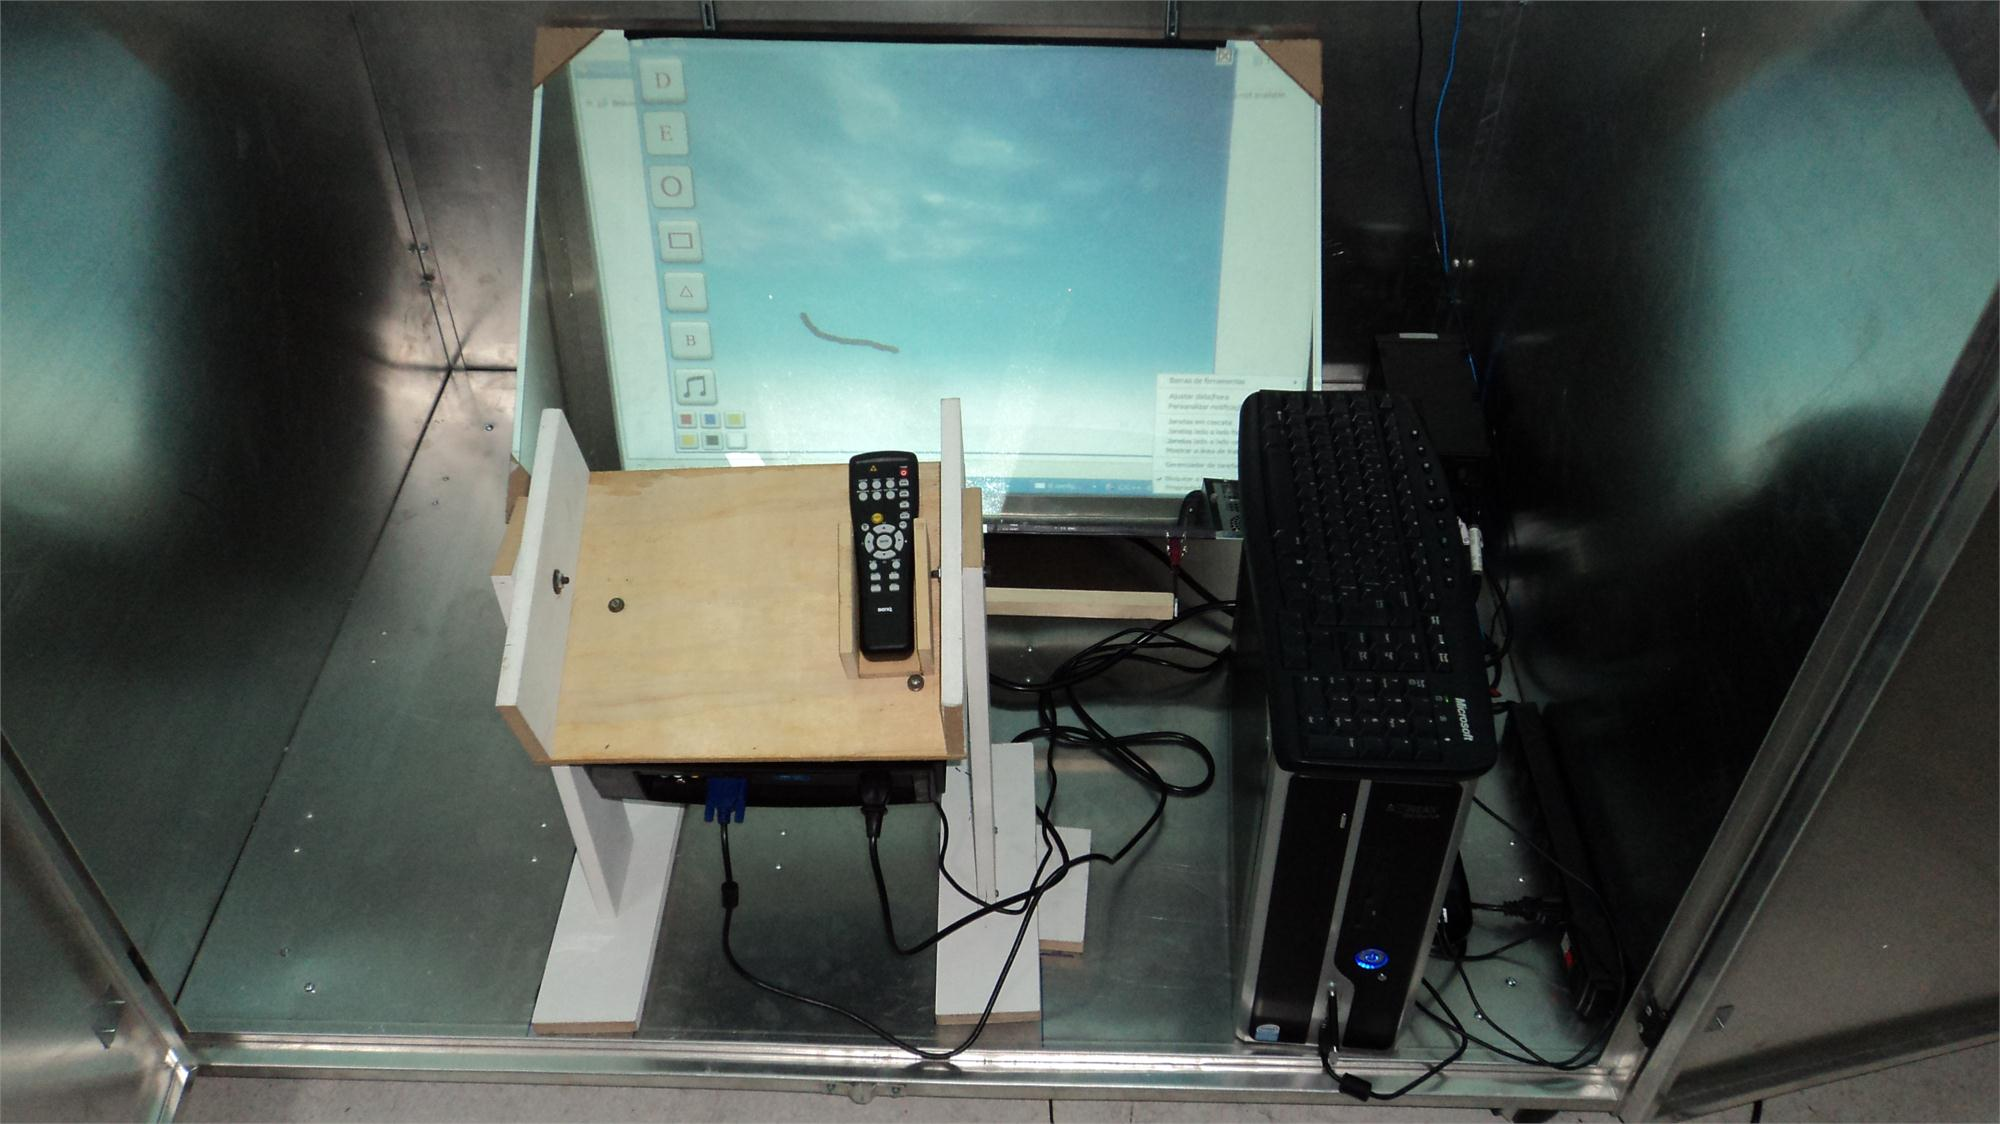
\includegraphics[scale=0.1]{mesapordentro.jpg}
	\caption{Vis�o interna da mesa, ilustrando seus componentes.}
	\label{mesadentro}
	\end{center}
\end{figure}

\begin{figure}[h!]
	\begin{center}
	\includegraphics[scale=0.1]{ps3eyenosuporte.jpg}
	\caption{C�mera \textit{Playstation Eye} no suporte.}
	\label{ps3eyenosuporte}
	\end{center}
\end{figure}

\section{Superf�cie}
\label{cap4.2}

A superf�cie da mesa � feita de uma chapa de acr�lico transl�cido extrudado, que oferece uma alta resist�ncia e transpar�ncia a um custo acess�vel. Seu coeficiente de refra��o � adequada e permite a ilumina��o de toda superf�cie. Sua transpar�ncia permite a capta��o dos toques com clareza pela c�mera. O acr�lico tem dimens�es de 120 x 90 cm e espessura de 1cm. Para reter a proje��o � aplicado um papel vegetal sob a face interna do acr�lico. O objetivo desta � impedir que a luz do canh�o do projetor multim�dia reflita no acr�lico causando uma interfer�ncia detect�vel pela c�mera. Al�m disso, ele ajuda a destacar a ilumina��o dos dedos, quando comparadas a da m�o, facilitando a detec��o de toques.

\section{Ilumina��o Infravermelha}
\label{cap4.3}

Para um reconhecimento satisfat�rio dos toques, foi utilizado o m�todo de ilumina��o \textit{FTIR}, introduzido no cap�tulo anterior. Os \textit{LED}s infravermelhos foram posicionados em furos ao redor do acr�lico apontados paralelamente a sua superf�cie (Figura~\ref{furosacrilico}). Aproveitando a resist�ncia do acr�lico, furou-se a lateral do acr�lico a, aproximadamente, cada 1cm utilizando uma furadeira de bancada para o posicionamento e fixa��o dos \textit{LED}s. Foram realizados 200 furos no total, 115 em um dos lados da mesa com 120cm e 85 em um dos lados com 90cm. Os \textit{LED}s foram ent�o inseridos nos furos e soldados (Figura~\ref{ledsolda}). Os \textit{LED}s s�o diodos de 5mm de di�metro com pot�ncia 1,1w m�xima, tendo a sua tens�o m�xima 5V e corrente 220mA. Como � utilizada uma fonte de 12,2V, eles foram soldados de acordo com o diagrama da Figura~\ref{diagftir}, com s�ries de 8 \textit{LED}s e um resistor para regular a corrente, todas essas s�ries em paralelo entre si.

\begin{figure}[h!]
	\begin{center}
	\includegraphics[scale=0.08]{furosacrilico(b).jpg}
	\caption{Furos efetuados na borda do acr�lico.}
	\label{furosacrilico}
	\end{center}
\end{figure}

\begin{figure}[h!]
	\begin{center}
	\includegraphics[scale=0.08]{ledsolda.jpg}
	\caption{\textit{LED}s soldados na borda do acr�lico.}
	\label{ledsolda}
	\end{center}
\end{figure}

\begin{figure}[h!]
	\begin{center}
	\includegraphics[scale=1]{circuito.jpg}
	\caption{Esquema de montagem do circuito dos \textit{LED}s infravermelhos.}
	\label{diagftir}
	\end{center}
\end{figure}


\section{C�mera}
\label{cap4.4}

Para capturar a imagem a ser processada de modo a identificar os toques sobre a superf�cie, foi utilizada uma c�mera \textit{PlayStation Eye}, que pode ser observada na Figura~\ref{ps3eyenosuporte}. A escolha foi baseada no baixo custo da c�mera, sua alta resolu��o para sua faixa de pre�o, �ngulo de abertura, pois permite a captura de imagens da superf�cie inteira com apenas uma c�mera, e a alta taxa de frames por segundo. Sua resolu��o pode ser configurada em 640 x 480 \textit{pixels}, ou em 320 x 240 \textit{pixels} numa taxa de atualiza��o de 75 ou 120 frames por segundo, respectivamente.

Para capturar os movimentos sobre a mesa com maior precis�o, modificou-se a c�mera de modo a permitir a filtragem do espectro de luz vis�vel e captar apenas luz infravermelha. Isto foi feito primeiro removendo o filtro nativo que a c�mera possui, que bloqueava a ilumina��o infravermelha, e depois aplicando-se um filme fotogr�fico sobre a lente da c�mera.

\section{Projetor}
\label{cap4.5}

Nesta mesa, o projetor utilizado � da marca \textit{BenQ} modelo \textit{MP772ST} (Figura~\ref{projetor}). Trata-se de um projetor \textit{WXGA}(\textit{Wide eXtended Graphics Array}) de resolu��o padr�o 1024x768 pixels com suporte a proje��o at� 1080i. O projetor foi posicionado a uma dist�ncia de 90cm da superf�cie do acr�lico. O projetor � fixado ao fundo da mesa e utiliza-se de um espelho para refletir a imagem at� o topo, sobre o papel vegetal que se encontra diretamente abaixo da chapa de acr�lico.

\begin{figure}[h!]
	\begin{center}
	\includegraphics[scale=0.4]{BENQ_MP772_ST.jpg}
	\caption{Projetor multim�dia \textit{BenQ MP772ST}~[\citenum{projpic}]}
	\label{projetor}
	\end{center}
\end{figure}

\section{Filtros de Processamento de V�deo}
\label{cap4.6}

Para detectar corretamente os toques, � necess�rio processar cada imagem recebida pela c�mera de forma a separar os toques das interfer�ncias das imagens de fundo. Para isso, utilizou-se uma cadeia de filtros dispon�veis na biblioteca \textit{Community Core Vision} (\textit{CCV})~[\citenum{ccv}].

\begin{figure}[h!]
	\centering
	\mbox{\subfigure[Captura sem filtro]{\includegraphics[scale=0.25]{filtro1.png}}
	\quad
	\subfigure[Filtro de \textit{Background}]{\includegraphics[scale=0.25]{filtro3.png}}
	\quad
	\subfigure[Filtro de \textit{Highpass}]{\includegraphics[scale=0.25]{filtro4.png}}}
	\mbox{\subfigure[Filtro \textit{Amplify}]{\includegraphics[scale=0.25]{filtro5.png}}
	\quad
	\subfigure[Filtro \textit{Rectify}]{\includegraphics[scale=0.25]{filtro6.png}}}
	\caption{Aplica��o dos filtros � imagem capturada pela c�mera do sistema.}
	\label{filtros}
\end{figure}

A Figura~\ref{filtros}(a) mostra a captura direta da c�mera, sem nenhum filtro de processamento aplicado, apenas o filtro de hardware apresentado na Se��o~\ref{cap4.4}. Na Figura~\ref{filtros}(b), pode-se ver o filtro de \textit{Background}, que guarda uma imagem inicial como refer�ncia e depois subtrai as imagens subsequentes, de modo a remover grande parte da interfer�ncia do fundo e de imperfei��es do acr�lico. Em seguida, na Figura~\ref{filtros}(c), � aplicado o filtro de \textit{Highpass}, que aumenta a luminosidade dos pontos que est�o a determinada dist�ncia da c�mera, removendo a luminosidade de pontos al�m destes, de modo a reduzir ru�dos. J� na Figura~\ref{filtros}(d), tem-se o filtro \textit{Amplify}, que intensifica a imagem obtida at� o momento, proporcionando \textit{blobs} brilhosos e de f�cil detec��o. Finalmente, na Figura~\ref{filtros}(e), � aplicado o filtro \textit{Rectify}, elimina pequenas interfer�ncias restantes, pois filtra \textit{blobs} abaixo de um certo n�vel de tamanho. Neste caso, � imprescind�vel que somente os toques estejam vis�veis, pois esta � a imagem usada para detect�-los.
\chapter{\textit{Software Deskworld}}
\label{cap5}

Neste cap�tulo � apresentado o \textit{design} do \textit{Software Deskworld} e seus detalhes de implementa��o, tais como arquitetura e a estrutura empregada.

\section{\textit{Design} do \textit{Deskworld}}
\label{cap5.1}

Nesta se��o, apresenta-se o \textit{design} do \textit{Software}, isto �, o projeto de sua aplica��o com as caracter�sticas expressas em uma vis�o computacional de alto n�vel, ou seja, a n�vel de usu�rio.

\subsection{Requisitos de interface}
\label{cap5.1.1}

De maneira simplificada, os requisitos de interface do \textit{Deskworld} podem ser expressos da seguinte forma:
\begin{itemize}
	\item sua mec�nica deve permitir a participa��o de diversos jogadores simultaneamente;
	\item deve suportar e processar toques simult�neos;
	\item deve possuir capacidade de aproximar linhas.
\end{itemize}

\subsection{Conceito}
\label{cap5.1.2}
O simulador de f�sica \textit{Deskworld} tem como principal proposta deixar a cargo da criatividade do(s) usu�rio(s) a constru��es de cen�rios, objetos e seus respectivos objetivos em seu mundo virtual. A meta principal � prover ferramentas aos usu�rios, auxiliando-os nessa constru��o. Assim, objetos e elementos f�sicos s�o representados em um plano bidimensional, regidos pelas leis da f�sica. � poss�vel desenhar um objeto e modificar suas propriedades tais como massa, coeficiente de atrito e elasticidade. O usu�rio pode aplicar uma for�a a este objeto como a gravidade, fix�-lo no plano, entre outras op��es. Pode-se ainda, alterar as propriedades do mundo em que se encontra e, sem interrup��es, divid�-lo, criando novos submundos para interagir separadamente.

\subsection{Regras e Objetos}
\label{cap5.1.3}
Basicamente, pode-se criar qualquer tipo de objeto 2D, com ou sem o aux�lio das ferramentas fornecidas. A constru��o funciona similarmente ao desenho virtual, onde o dedo representa o l�pis e a superf�cie da mesa o papel. Os objetos podem ser criados de forma livre, ou com aux�lio do software que tenta aproximar os desenhos do usu�rio a linhas retas, facilitando a constru��o de pol�gonos.

Para a altera��o de regras do mundo, ferramentas utilizadas ou propriedades dos objetos, o usu�rio possui um menu, que pode ser acessado atrav�s de dois toques subsequentes em um local da tela. Os itens do menu podem ser selecionados com um �nico toque neles.

Cada objeto pode ter as seguintes caracter�sticas:
\begin{itemize}
	\item Densidade
	\item Coeficiente de atrito
	\item Coeficiente de restitui��o de for�a
	\item For�a normal
	\item Massa
	\item Volume
	\item Velocidade
\end{itemize}

Dentre as caracter�sticas acima, a densidade, o coeficiente de atrito, o coeficiente de restitui��o de for�a e a massa podem ser alterados pelo usu�rio a qualquer momento, utilizando o menu.

Al�m dessas propriedades, os objetos podem interagir entre si por meio de juntas, colis�es ou motores adicionados aos objetos, que aplicam uma for�a constante sobre um objeto. As juntas s�o entidades que permite fixar um objeto a outro. Funciona, analogamente, a colocar um prego para juntar dois peda�os de madeira. Tamb�m � poss�vel a separa��o de mundos com gravidades diferentes e cores de pinc�is diferentes entre si.

Neste \textit{software} interativo, n�o existem regras pr�-definidas. Fica a crit�rio do usu�rio definir suas regras enquanto interage com o \textit{software} criando cen�rios e objetos.

\subsection{Interface}
\label{cap5.1.4}
A interface utilizada para testes � a mesa cuja constru��o foi descrita no Cap�tulo~\ref{cap4}. Entretanto, salienta-se que o \textit{software Deskworld} � port�vel para qualquer interface multi-toque que suporte o protocolo \textit{TUIO}.

\section{Ferramentas de suporte}
\label{cap5.2}

Nesta se��o, ser�o descritas as ferramentas de suporte utilizadas na constru��o do simulador \textit{Deskworld}, tais como game engine e bibliotecas.

\subsection{\textit{Game Engine}}
\label{cap5.2.1}

A \textit{engine} utilizada no desenvolvimento deste software foi a Box2D~[\citenum{Box2Dmanual}]. A principal funcionalidade da \textit{Box2D}, no contexto desse \textit{software}, foi auxiliar na cria��o dos objetos e no tratamento de eventos relacionados � simula��o das leis da f�sica. Tais eventos s�o:

\begin{itemize}
	\item Gravidade
	\item Colis�o
	\item For�a de a��o e rea��o
	\item For�a de atrito
\end{itemize}

Al�m dessas funcionalidades, a \textit{Box2D} � respons�vel pela ger�ncia de mem�ria, jun��o de objetos e/ou a fixa��o deles.

\subsection{\textit{Bibliotecas de apoio}}
\label{cap5.2.2}

Para facilitar a implementa��o do \textit{software}, foram utilizadas diversas bibliotecas. Uma das bibliotecas padr�o do C++, a \textit{STL} \textit{(Standart Template Library)}, possui algumas estruturas complexas de dados j� implementadas, sendo amplamente utilizada neste simulador. Para a parte gr�fica do jogo foi utilizada a biblioteca \textit{SDL}~[\citenum{sdl}]  \textit{(Simple Direct Layer)} em conjunto com a \textit{OpenGL}~[\citenum{opengl}]  (\textit{Open Graphics Library}). Com rela��o ao �udio, utilizou-se a biblitoca \textit{SDL\_mixer}~[\citenum{sdlmixer}] . Para tratamento de \textit{input} foi utilizada a biblioteca do protocolo \textit{TUIO}~[\citenum{TUIO}] (\textit{Tangible User Interface System}).

\subsubsection{\textit{SDL} e \textit{OpenGL}}
\label{cap5.2.2.1}

Por oferecer uma boa abstra��o de \textit{hardware}, ser bem difundida no mercado de jogos e possuir ampla documenta��o, utilizou-se a \textit{SDL} para disponibilizar o acesso ao ambiente. Em conjunto com a \textit{SDL}, na parte gr�fica, foi utilizada a \textit{OpenGL} (\textit{Open Graphics Library}), que realiza a renderiza��o das imagens.

A \textit{SDL\_mixer} � utilizada para permitir a reprodu��o de diversas faixas de �udio simultaneamente.

\subsubsection{Protocolo \textit{TUIO}}
\label{cap5.2.2.2}

A comunica��o entre o usu�rio da mesa e o aplicativo � realizada de acordo com o protocolo \textit{TUIO}~[\citenum{TUIO}] (\textit{Tangible User Interface System}). Este protocolo � especificado para atender as necessidades de comunica��o das interfaces tang�veis, que s�o interfaces sens�veis ao toque, capazes de serem controladas por movimentos corporais e gestos. A implementa��o � simples e visa melhorar a performance na comunica��o. Para isso, ele opera sobre a camada \textit{UDP}(\textit{User Datagram Protocol}) de transporte utilizando tr�s tipos de mensagens: \textit{set}, \textit{alive} e \textit{fseq}. As mensagens \textit{set} s�o utilizadas para informar o estado de um objeto. Mensagens \textit{alive} indicam o conjunto de objetos presentes na interface atrav�s de uma identifica��o �nica atribu�da a cada novo elemento reconhecido. Mensagens \textit{fseq} s�o transmitidas antes da etapa de atualiza��o de cada quadro, para marc�-lo unicamente, associando-o a cada mensagem \textit{set} e \textit{alive}. A seguir � apresentado um  resumo do funcionamento do protocolo:

\begin{itemize}
	\item Par�metros do objeto s�o enviados ap�s mudan�a de estado, por interm�dio da mensagem \textit{set}.
	\item Objetos removidos da interface s�o comunicados por meio de mensagens \textit{alive}.
	\item Cliente deduz a lista de objetos adicionados e removido por meio das mensagens \textit{set} e \textit{alive}.
	\item Mensagens \textit{fseq} associam um ID a um conjunto de mensagens \textit{set} e \textit{alive} do quadro.
\end{itemize}

Apesar da camada UDP de transporte n�o oferecer garantia de entrega dos dados, o TUIO implementa redund�ncia de informa��o para se precaver contra a perda de dados na transmiss�o. Al�m disso, o estado de um objeto, mesmo inalterado, � enviado periodicamente em uma mensagem \textit{set}. Portanto, o protocolo � ideal para ser utilizado em aplicativos controlados por interfaces multitoque, otimizando a intera��o e confiabilidade da comunica��o. Na Tabela~\ref{tab:tabela1_param_TUIO}, pode-se observar todos os par�metros que s�o enviados a cada mensagem do protocolo \textit{TUIO}.

\begin{table}[htbp]
  \centering
  	\caption{Par�metros de mensagens TUIO em superf�cies interativas 2D}
    \begin{tabular}{|l|l|l|} %rrr}
    \textbf{Par�metros} & \textbf{Significado dos par�metros} & \textbf{Tipo} \\
    s     & sessionID (ID tempor�rio do objeto) & int32 \\
    x, y  & posi��o & float32 \\
    X, Y  & vetor de movimento (velocidade de movimento e dire��o) & float32 \\
    m     & acelera��o de movimento & float32 \\
    w, h  & largura e altura do \textit{blob} & float32 \\
    \end{tabular}%
  \label{tab:tabela1_param_TUIO}%
\end{table}%

\subsubsection{\textit{Community Core Vision}}
\label{cap5.2.3}

\begin{figure}[h!]
	\begin{center}
	\includegraphics[scale=0.4]{ccv.jpg}
	\caption{Aplicativo de captura de toques \textit{Community Core Vision}~[\citenum{ccv}]}
	\label{ccv}
	\end{center}
\end{figure}

O \textit{CCV} (\textit{Community Core Vision})~[\citenum{ccv}] � um aplicativo para auxiliar no processamento de imagens capturadas pela c�mera em intera��es com superf�cies multi-toque. A Figura~\ref{ccv} apresenta um \textit{screenshot} do aplicativo. Ele lida com o acompanhamento dos \textit{blobs} de luz infravermelha, enviando mensagens para o \textit{Deskworld}, tais como o encostar do dedo, o deslocar do dedo e o retirar do dedo. Interage com a maioria dos dispositivos de captura de v�deo, sendo muito �til para um projeto de software que utilize uma mesa multitoque.  Atualmente, possui suporte para plataformas \textit{Windows} e \textit{Linux}, 32 ou 64 \textit{bits}, e \textit{MacOS}.

Seu funcionamento consiste na aplica��o de filtros configur�veis, como os mostrados na Figura~\ref{filtros} no cap�tulo anterior. Em seu arquivo de configura��o, \textit{config.xml}, pode-se modificar os dados da c�mera, tais como resolu��o e frames por segundo; o \textit{CCV} ir� automaticamente ajustar a c�mera selecionada para os dados mais pr�ximos suportados. A execu��o do \textit{CCV} funciona de acordo com o paradigma cliente-servidor, onde o mesmo atua como servidor e a aplica��o como cliente. Esta comunica��o cliente-servidor � feita utilizando o protocolo TUIO~[\citenum{TUIO}] \textit{(Tangible User Interface System)}, utilizando pontos normais x e y enviados via \textit{TCP}, ou em pacotes especiais para aplicativos \textit{Flash}, permitindo uma arquitetura distribu�da, onde o aplicativo � executado separadamente da aplica��o de processamento de imagens.

\section{Arquitetura e Detalhes de Implementa��o}
\label{cap5.3}

A evolu��o da tecnologia dos \textit{hardwares} para computadores pessoais proporcionou grande desenvolvimento � ind�stria de jogos eletr�nicos, levando-a a aprimorar seu produto ao longo do tempo. Este caminho foi marcado pela forma��o de grandes equipes e pela extensiva carga de codifica��o. Os jogos eletr�nicos mais modernos podem ultrapassar um milh�o de linhas de c�digo de acordo com \textit{Rabin et al.}~[\citenum{I2GMDVP}]. Portanto, foi necess�rio organizar estes extensivos c�digos a fim de obter uma melhor performace no desenvolvimento de novos jogos. Esta organiza��o pode ser realizada por meio da ado��o de uma arquitetura bem definida.

\subsection{Arquitetura do \textit{Deskworld}}
\label{cap5.3.1}

Apesar de n�o se encaixar na defini��o de jogo eletr�nico, o \textit{Deskworld} possui muitas caracter�sticas semelhantes, pois � um \textit{software} interativo, onde o usu�rio se relaciona com objetos em um mundo virtual. Dessa maneira, este \textit{software} foi desenvolvido a partir da utiliza��o de um padr�o de desenvolvimento voltado a jogos. Para este \textit{software} foi escolhida uma arquitetura modular orientada � objetos.

\subsubsection{Vantagens da abordagem orientada � objetos}
\label{cap5.3.1.1}

De acordo com \textit{Rabin et al.}~[\citenum{I2GMDVP}] a maioria dos jogos se desenvolvem em torno de objetos ou entidades em um mundo virtual, nos quais o usu�rio deve realizar a��es. Antes da exist�ncia do paradigma da orienta��o a objetos, os jogos eram desenvolvidos com programa��o procedural e assim, a �nfase da programa��o baseava-se no c�digo propriamente dito. Isto porque o jogo era observado, conceitualmente, como uma sequ�ncia de c�digo com execu��o de procedimentos e fun��es. Na programa��o orientada � objetos, a perspectiva � outra, pois a �nfase ocorre no conceito de objeto que � uma cole��o de informa��es conjuntas a uma s�rie de opera��es para processar estes dados. Portanto, utilizando orienta��o � objetos � poss�vel obter \textit{softwares} que se adequam ao formato dos jogos, pois as entidades desses jogos podem ser expressas pelas classes, os objetos por inst�ncias da classe e a��es entre eles pelos m�todos.

Outra vantagem encontrada nesta abordagem � a heran�a de classes, que permite a reutiliza��o de c�digo em m�ltiplas classes que possuam parentesco. Com heran�a, � poss�vel estender caracter�sticas das superclasses para as subclasses. No \textit{Deskworld}, utilizou-se heran�a para, principalmente, padronizar e reutilizar parte do c�digo dos \textit{Game Objects}. Tamb�m importante, o suporte ao polimorfismo � crucial no desenvolvimento de jogos j� que permite a realiza��o de \textit{update} e \textit{render} de diversos componentes do \textit{software} sem precisar separ�-los em chamadas de execu��es diferentes, pois todos ser�o reconhecidos pelo seu tipo e ter�o seus respectivos m�todos executados corretamente.

A arquitetura do programa foi modularizada para especificar claramente os  seus subsistemas, facilitando a manuten��o e o entendimento do c�digo. No diagrama apresentado na Figura~\ref{diag-deskworld} pode ser observada a composi��o de m�dulos do \textit{Deskworld} e suas principais classes. A decomposi��o em m�dulos facilita a visualiza��o da implementa��o, j� que o \textit{software} possui subsistemas bem claramente definidos como os de �udio, v�deo, \textit{engine} e de \textit{input}.

\subsection{Detalhes de implementa��o}
\label{cap5.3.2}

Esta se��o apresenta a l�gica de implementa��o do \textit{software}. Primeiramente, � exposto uma vis�o geral do funcionamento do sistema. Em seguida, os subsistemas s�o detalhados e seus pap�is tra�ados.

\subsubsection{Vis�o Geral do \textit{Software}}
\label{cap5.3.2.1}

Como observado no diagrama da Figura~\ref{diag-deskworld}, existe uma classe \textit{Game Manager} respons�vel pelo gerenciamento da execu��o do programa. Suas principais a��es s�o inicializar os subsistemas de �udio, v�deo, carregar o cen�rio e inicializar a \textit{Engine} do \textit{Deskworld}. A classe �udio � respons�vel por carregar arquivos de �udio, bem como manipul�-los, podendo tocar, parar ou resumir um arquivo carregado. A \textit{Graphics} implementa solu��es para renderizar os objetos na tela e gerenciar a mem�ria de v�deo. O \textit{InputManager} trata as mensagens de entrada recebidas, explorados na Se��o~\ref{cap5.2.2.2}, e gera eventos relativos aos toques. A \textit{Engine} tem como objetivo criar, alterar e posicionar objetos no mundo, al�m de se comunicar de posse destas informa��es  com a \textit{Box2D}. A classe \textit{LevelState} concentra o maior fluxo de informa��es, pois todas as inst�ncias de classe de objetos do mundo s�o criada nela. Os m�todos de \textit{Update}, muito importante em simula��es f�sicas, e \textit{Render} t�m suas chamadas realizadas pelo \textit{LevelState}. O \textit{Game Object} armazena informa��es sobre os objetos como sua dimens�o, posi��o e estado.

\begin{figure}[h!]
	\begin{center}
	\includegraphics[scale=0.35]{DeskworldDiagram.png}
	\caption{Diagrama de classes do \textit{Deskworld}}
	\label{diag-deskworld}
	\end{center}
\end{figure}

\subsubsection{Subsistemas de �udio e V�deo}
\label{cap5.3.2.2}

O subsistema de �udio possui atributos para identificar o nome do arquivo de �udio, o tipo do arquivo e um ponteiro para seu endere�amento na mem�ria. Seu construtor carrega o arquivo de �udio para mem�ria e retorna esse endere�o ao ponteiro da classe. Utiliza-se esta classe para tocar e pausar a m�sica de fundo. 

A classe \textit{Graphics} gerencia a mem�ria de v�deo com a \textit{OpenGL}, e a utiliza para desenhar formas geom�tricas na tela. A classe \textit{ImageLoader} carrega imagens e texturas e renderiza-as. As texturas presentes no \textit{Software} s�o o fundo, menu e seus componentes.

\textbf{\textit{Singleton}}

A classe \textit{Graphics} � um \textit{Singleton}, isto �, possui, obrigatoriamente, apenas uma inst�ncia durante todo o programa. \textit{Singleton} � um \textit{design pattern} muito utilizado em situa��es que necessitam de grande controle sobre uma classe para que seja instaciada somente uma vez. Esta t�cnica consiste em declarar um construtor privado que ser� executado uma �nica vez. Constr�i-se um m�todo que retorna a inst�ncia �nica por meio de um ponteiro est�tico. Caso seja a primeira vez que � chamado, a classe � instanciada, caso contr�rio, retorna a inst�ncia j� existente. Al�m desta, o \textit{InputManager} e a \textit{Engine} s�o singletons. Isto acontece porque todas essas classes s� devem possuir somente uma inst�ncia, pois n�o se deseja v�rias inst�ncias controlando a sa�da de v�deo, a entrada de dados ou a simula��o de objetos.

\subsubsection{Subsistema de \textit{Input}}
\label{cap5.3.2.3}

Neste subsistema, para dar suporte ao protocolo TUIO, tem-se a classe \textit{InputManager}, derivada da classe \textit{TuioListener}, que implementa m�todos para escutar mensagens relativas � detec��o de toques, gerando eventos. Estes eventos podem adicionar e remover toques ou atualizar suas posi��es. Tamb�m suporta a detec��o de eventos de input via mouse ou teclado. O m�todo principal da classe � o \textit{Update}, onde s�o percorridos todos os eventos enviados durante um \textit{Game Loop}, cada um sendo analisado e seus dados separados para utiliza��o das outras classes. Por exemplo, caso seja adicionado um toque, o n�mero identificador deste toque � salvo, permitindo que outra classe possa utiliz�-lo por meio do m�todo \textit{IsTouching}, de modo a descobrir se o toque com o identificador desejado est� tocando ou n�o a superf�cie.

\subsubsection{Subsistema da \textit{Engine}}
\label{cap5.3.2.4}

A \textit{Engine} � composta pela classe \textit{Engine}, al�m do pacotes de classes da biblioteca \textit{Box2D}. Por interm�dio destas classes, ocorre a cria��o dos objetos no mundo virtual. A simula��o de gravidade, da for�a de atrito, e das for�as de a��o e rea��o, s�o calculadas pela \textit{Engine}. Um importante recurso para uma boa simula��o � a detec��o de colis�o, tratada por esse subsistema. Tamb�m s�o realizadas opera��es de destrui��o de objetos, al�m da localiza��o dos objetos ser atualizada e repassada aos outros m�dulos pela \textit{Engine}.

\subsubsection{Subsistema de ger�ncia de objetos}
\label{cap5.3.2.5}

A classe \textit{LevelState} � respons�vel pelo �nico estado do \textit{software}. Estar no estado de \textit{LevelState} significa que o \textit{software} est� em execu��o e o usu�rio pode interagir como desejar, criando objetos ou mudando propriedades. Nesta classe, todas as imagens que aparecem dentro do jogo s�o carregadas e renderizadas na tela. Seu m�todo de \textit{Update}, chamado uma vez pelo \textit{Game Loop}, verifica todos os toques existentes ou removidos e decide o que cada um ir� fazer, como por exemplo, criar um objeto novo, arrastar um objeto existente, abrir o menu ou alterar as op��es. Seu outro m�todo, \textit{Render}, � respons�vel por montar a tela do jogo, renderizando na tela todas as imagens em sua sequ�ncia, deixando-as prontas para serem mostradas na tela, assim que tudo estiver em posi��o.

A \textit{GameObject} � uma superclasse que agrega subclasses referentes a todos objetos presentes \textit{software}. Estas classes representam os objetos desenhados no programa que podem ser pol�gonos, c�rculos ou terem forma livre. Al�m disso, objetos podem ser motores e juntas. O pr�prio mundo � um objeto, pois podem existir v�rios mundos, e as pr�prias barreiras usadas para dividir entre submundos tamb�m s�o consideradas objetos. Todos objetos possuem v�rtices que indicam suas posi��es e suas �reas. Todos os \textit{GameObject}s possuem m�todos de \textit{Update} e \textit{Render}.
%\chapter{Arquitetura e Detalhes de Implementa��o}
\label{cap6}

\section{Arquitetura do jogo}
\label{cap6.1}

A evolu��o da tecnologia dos hardwares dos computadores pessoais proporcionou grande desenvolvimento � ind�stria de jogos eletr�nicos levando-a a aprimorar seu produto ao longo do tempo. Este caminho foi marcado por grandes equipes e pela extensiva codifica��o. Os jogos eletr�nicos mais modernos podem ultrapassar um milh�o de linhas de c�digo de acordo com \textit{Rabin et al.}~[\citenum{I2GMDVP}]. Portanto, foi necess�rio organizar estes extensivos c�digos a fim de obter melhor performace no desenvolvimento de novos jogos. Esta organiza��o pode ser realizada por meio da ado��o de uma arquitetura bem definida.

Para este jogo escolhemos uma arquitetura de desenvolvimento baseada em um sistema de componentes.

\subsection{Sistema de Componentes}
\label{cap6.1.1}

Um sistema de componentes � caracterizado pela sua estrutura n�o-hier�rquica. O jogo que se baseia em componentes ter� somente uma classe pai que representar� todas as entidades do jogo, enquanto quaisquer outras classes ser�o irm�s entre si, pois todas ser�o filhas da entidade do jogo. Cada classe filha da entidade � um componente, ou seja, o entidade do jogo � formada por uma composi��o de componentes.

� observado a independ�ncia de cada componente, onde podemos, por exemplo, ter a liberdade de transformar um elemento de uma classe jogador em ve�culo. Entretanto, mesmo com a mudan�a podemos manter a coer�ncia l�gica do jogo, pois estas classes ter�o a mesma estrutura que forma a entidade do jogo, como audio, corpo f�sico e apar�ncia.

\begin{figure}[h!]
	\begin{center}
	\includegraphics[scale=0.8]{componente.png}
	\caption{Exemplo de uso de componentes em entidades de jogo~[\citenum{pedrosaulo}]}
	\label{componente}
	\end{center}
\end{figure}

\subsection{Vantagens em rela��o ao sistema hier�rquico}
\label{cap6.1.2}

Um sistema baseado em componentes � uma alternativa ao forte acomplamento provocado pela hierarquia de classes. Em linguagens orientadas � objeto a hierarquia de classes pode ser de grande ajuda como pode dificultar a codifica��o do software. Isto porque, em sistemas onde temos tipos de objetos pr�-definidos, assim como as rela��es entre eles, a hierarquia pode ser de grande ajuda. Isto acontece pelo fato da f�cil representa��o do jogo como um hierarquia. Por exemplo, em jogos de esporte, geralmente, temos caracter�sticas fortemente consolidadas. Um jogador de basquete, dificilmente, se transformar� em uma bola. A forte acopla��o entre as classes favorece a implementa��o de uma arquitetura hierarquizada.

\begin{figure}[h!]
	\begin{center}
	\includegraphics[scale=0.65]{hierarquia.png}
	\caption{Exemplo de uso de hierarquia em entidades de jogo~[\citenum{pedrosaulo}]}
	\label{hierarquia}
	\end{center}
\end{figure}

No entanto, no caso do jogo \textit{DeskWorld} teremos problemas se utilizarmos este tipo de arquitetura. Isto porque, de acordo com \textit{Rabin et al.}~[\citenum{I2GMDVP}], uma arquitetura majoritariamente baseada em hierarquia de classes possui significantes limita��es. Uma de suas principais � a baixa flexibilidade devido ao forte acomplamento. O fato de termos classes hier�rquicas gera a depend�ncia \textit{inter-classe}, j� que, parte de suas caracter�sticas s�o herdadas de uma classe, sendo que, mudan�as realizadas em caracter�sticas de uma classe refletiram sobre suas filhas.

Outro ponto apresentado em~[\citenum{I2GMDVP}], � que, em linguagens bem difundidas no desenvolvimento de jogos, como \textit{C++} e \textit{Java}, a estrutura modelada em hierarquia � est�tica, n�o permitindo a altera��o de classes em tempo de execu��o. Isto pode ser um grande entrave, pois certos jogos podem realizar diversas altera��es dr�sticas no comportamento de entidades. Podemos exemplificar esse ponto tomando um jogo em que a morte de um certo inimigo possa se transformar em um item ou dinheiro.

\subsection{Comunica��o entre componentes}
\label{cap6.1.3}

Para aproveitar a flexibilidade provida pelo sistema de componentes, necessitamos realizar a comunica��o entre componentes, visto que, ser� a respons�vel por engatilhar a transforma��o de uma entidade. � a mensagem que avisar� ao objeto que seu comportamento ir� ser alterado e associado a uma outra classe.

Esta comunica��o pode ficar a cargo da entidade do jogo, onde, por exemplo, pode realizar a transfer�ncia de um som de uma classe de �udio para uma classe ve�culo. Num sistema simples, essa comunica��o pode ser implementada por uma simples chamada de fun��o onde ponteiros s�o passados refer�nciando suas respectivas caracter�sticas.

\section{\textit{Design Patterns}}
\label{cap6.2}

\textit{Design Patterns} s�o padr�es de projeto de orienta��o a objetos que visam reconhecer padr�es recorrentes de forma a aumentar a flexibilidade e permitir o reuso do c�digo se usados de forma adequada. Isso se d� pois o seu uso aumenta a indep�ndencia dos sistemas, o que tamb�m aumenta a capacidade de evolu��o do c�digo em si.

Como foi descrito em~[\citenum{pedrosaulo}], para cada padr�o, s�o estabelecidos os seguintes aspectos:
\begin{itemize}
	\item{O \textbf{nome} usado para descrever, de maneira sucinta e precisa em no m�ximo duas palavras, o problema, a solu��o e as consequ�ncias inerentes do padr�o.}
	\item{O \textbf{problema} e o contexto adequados para a aplica��o do padr�o.}
	\item{A \textbf{solu��o} descreve os elementos que comp�em o padr�o. Cada solu��o inclui relacionamentos entre classes e a colabora��o entre estes casos existam.}
	\item{As \textbf{consequ�ncias} de se aplicar o padr�o, ou seja, os resultados e as desvantagens.}
\end{itemize}

Gra�as ao fato de jogos serem extremamente modulares, eles ganham um grande benef�cio por utilizar alguns padr�es de projeto. Abaixo est�o explicados os mais utilizados para este prop�sito.

\subsection{\textit{Singleton}}
\label{cap6.2.1}

\begin{figure}[h!]
	\begin{center}
	\includegraphics[scale=1]{singleton.png}
	\caption{Padr�o \textit{Singleton}~[\citenum{pedrosaulo}]}
	\label{singleton}
	\end{center}
\end{figure}

O padr�o \textit{Singleton} trata de um padr�o aonde uma classe necessita necessariamente ser �nica durante todo o programa, mesmo ela podendo ser utilizada em v�rias situa��es.

Atrav�s desse padr�o, a classe \textit{Singleton} cuida para que ela seja instanciada somente uma vez. Podemos verificar a implementa��o desse padr�o na figura~[\ref{singleton}], onde temos uma opera��o de classe, 'Instance()', que retorna a �nica inst�ncia, e � salvo como ponteiro est�tico dessa classe. Caso seja a primeira vez que � chamado, a classe � instaciada, caso contr�rio, retorna a inst�ncia j� existente. O construtor � privado para que a classe n�o possa ser criada por fora dela.

Em jogos, o padr�o \textit{Singleton} � muito usado para controlar eventos e gerenciar mensagens, bem como controlar recursos. Em todos esses casos, apensa uma inst�ncia pode existir e ela deve permitir acesso global a ela.

\subsection{\textit{Observer}}
\label{cap6.2.2}

\begin{figure}[h!]
	\begin{center}
	\includegraphics[scale=1]{observer.png}
	\caption{Padr�o \textit{Observer}~[\citenum{pedrosaulo}]}
	\label{observer}
	\end{center}
\end{figure}

O padr�o \textit{Observer}, visto na figura~[\ref{observer}], define um padr�o onde um objeto, chamado de \textit{subject}, mant�m uma lista de observadores e os notifica de mudan�as de estados. Quando a informa��o � passada, os observadores consultam o \textit{subject} para sincronizar os dados. O \textit{subject} n�o precisa conhecer detalhes do observador.

Utilizando a classe \textit{subject}, podemos adicionar ou remover observadores O observador, no entanto, define uma interface para objetos que notificam sobre sua altera��o para o subject. Essa � a �nica liga��o entre o observador e o \textit{subject}.

Este padr�o tamb�m � reconhecido na ind�stria de jogo. Como a arquitetura de jogos � marcada pela intera��o entre entidades distintas, o \textit{observer} deve ser usado. Assim as entidades se conhecem e aguardam receber atualiza��es de outras entidades que comp�em o seu meio ambiente.
%\chapter{Estrutura de implementa��o do simulador}
\label{cap7}

Neste cap�tulo, ser� descrito as ferramentas de suporte utilizadas na constru��o do simulador.

\section{\textit{Game Engine}}
\label{cap7.1}

A \textit{engine} utilizada neste jogo foi a \textit{Box2D}.Seu manual pode ser encontrado em~[\citenum{Box2Dmanual}]. A principal funcionalidade da \textit{Box2D} neste jogo foi auxiliar na cria��o dos objetos e no tratamento de eventos relacionados a simula��o das leis da f�sica. Estes eventos est�o apresentados abaixo:

\begin{itemize}
	\item Gravidade
	\item Colis�o
	\item For�a de a��o e rea��o
	\item For�a de atrito
	\item For�a de fric��o
\end{itemize}

Al�m dessas funcionalidades, a \textit{Box2D} � respons�vel pela ger�ncia de mem�ria, jun��o de objetos e/ou fixa��o deles.

\section{\textit{Bibliotecas de apoio}}
\label{cap7.2}

Para facilitar a implementa��o de foram utilizadas diversas bibliotecas. Uma das bibliotecas padr�o do C++ a STL \textit{(Standart Template Library)} possui algumas estruturas complexas de dados j� implementadas, sendo amplamente utilizada neste simulador. Para a parte gr�fica do jogo foi utilizada a biblioteca SDL \textit{(Simple Direct Layer)} conjuntamente com a \textit{OpenGL} (\textit{Open Graphics Library}). Com rela��o ao �udio, utilizou-se a SDL\_mixer. Para tratamento de \textit{input} foi utilizada a \textit{Touchlib}.

\subsection{SDL e \textit{OpenGL}}
\label{cap7.2.1}

Por oferecer uma boa abstra��o de \textit{hardware}, ser bem difundida no mercado de jogos e possuir ampla documenta��o, utilizou-se a SDL para disponibilizar o acesso ao ambiente \textit{OpenGL}. Conjuntamente com a SDL, na parte gr�fica, foi utilizado a \textit{OpenGL} (\textit{Open Graphics Library}) que realiza a renderiza��o das imagens.

A SDL\_mixer � utilizada para permitir a reprodu��o de diversas faixas de audio simultaneamente.

\subsection{Protocolo \textit{TUIO}}
\label{cap7.2.2}

Comunica��o entre o usu�rio da mesa com o aplicativo � realizada de acordo com o protocolo \textit{TUIO}~[\citenum{TUIO}] (\textit{Tangible User Interface System}). Este protocolo especificado para atender as necessidades da comunica��o das interfaces tang�veis. Interfaces tang�veis s�o interfaces sens�veis a toque, capazes de serem controladas por movimentos corporais e gestos. A implementa��o � simples e visa melhorar a performace na comunica��o. Para isso, ele opera sobre a camada UDP(\textit{User Datagram Protocol}) de transporte utilizando tr�s tipos de mensagens: \textit{set}, \textit{alive} e \textit{fseq}. Mensagens \textit{set} s�o utilizadas para informar o estado de um objeto. Mensagens \textit{alive} indicam o conjunto de objetos presentes na interface atrav�s de uma identifica��o �nica atribu�da a cada novo elemento reconhecido. Mensagens \textit{fseq} s�o transmitidas antes da etapa de atualiza��o de cada quadro para marcar-lo unicamente, associando-o a cada mensagem \textit{set} e \textit{alive} dele. Resumindo o funcionamento do protocolo:

\begin{itemize}
	\item Par�metros do objeto s�o enviados ap�s mudan�a de estado atrav�s da mensagem \textit{set}
	\item Objetos removidos da interface s�o comunicados atrav�s de mensagens \textit{alive}
	\item Cliente deduz a lista de objetos adicionados e removido por meio das mensagens \textit{set} e \textit{alive}
	\item Mensagens \textit{fseq} associam um ID a um conjunto de mensagens \textit{set} e \textit{alive} do quadro
\end{itemize}

Apesar da camada UDP de transporte n�o oferecer garantia de entrega dos dados, o TUIO implementa redund�ncia de informa��o para se precaver contra a perda de dados na transmiss�o. Al�m disso, o estado de um objeto, mesmo inalterado, � enviado periodicamente em uma mensagem \textit{set}. Portanto, o protocolo � ideal para ser utilizado em aplicativos controlados interfaces multitoques otimizando a itera��o e confiabilidade da comunica��o.

\textbf{\large{Par�metros das mensagens TUIO}}

\begin{table}[htbp]
  \centering
    \begin{tabular}{|l|l|l|} %rrr}
    \textbf{Parametros} & \textbf{Significado dos parametros} & \textbf{Tipo} \\
    s     & sessionID (ID tempor�rio do objeto) & int32 \\
    x, y  & posi��o & float32 \\
    X, Y  & vetor de movimento (velocidade de movimento e dire��o) & float32 \\
    m     & acelera��o de movimento & float32 \\
    w, h  & largura e altura do \textit{blob} & float32 \\
    \end{tabular}%
		\caption{Par�metros de mensagens TUIO em superf�cies interativas 2D}
  \label{tab:tabela1_param_TUIO}%
\end{table}%

\subsection{\textit{Touchlib}}
\label{cap7.2.3}

\textit{Touchlib}~[\citenum{Touchlib}] � uma biblioteca para auxiliar o processamento de imagens capturadas pela webcam em itera��es com superf�cies multitoque. Ela lida com o acompanhamento de \textit{blobs} de luz infravermelha, e envia para seus programas esses eventos multitoques, como o encostar do dedo, deslocamento do dedo e o retirar do dedo. Inclui um aplicativo de configura��o, algumas demos para exemplificar seu uso. Interage com a maioria dos tipos de webcams e os dispositivos de captura de v�deo sendo muito �til para um projeto de \textit{software} para mesa multitoque. Em contrapartida s� tem suporte para para sistema operacional \textit{Windows}.

Seu funcionamento consiste na aplica��o de filtros de forma customiz�vel como os mostrados nesta figura~[\ref{filtros}]. A execu��o destes filtros s�o realizadas pela \textit{Touchlib} com o uso da \textit{OpenCV (Open Source Computer Vision Library)}, uma biblioteca para o desenvolvimento de aplicativos de processamento de imagens. A execu��o da \textit{Touchlib} funciona de acordo com o paradigma cliente-servidor, sendo a mesma atuando como servidor e a aplica��o como cliente. Esta comunica��o cliente-servidor � feita utilizando o protocolo TUIO~[\citenum{TUIO}] \textit{(Tangible User Interface System)}, permitindo uma arquitetura distribu�da, onde o aplicativo � executado separadamente da aplica��o do processamento de imagens.

\chapter{Conclus�o}
\label{conclusao}

Existem diversos tipos diferentes de \textit{softwares} para mesas com superf�cie multi-toque, no entanto, s�o poucos que realmente aproveitam totalmente as capacidades de uma mesa multi-toque. Neste trabalho foi desenvolvido um \textit{software} simulador de f�sica, que devido a suas caracter�sticas consegue aproveitar bem o \textit{input} por toques e gestos e incentiva o uso de v�rios usu�rios ao mesmo tempo. Ao finalizar este projeto, conclu�mos que a escolha de \textit{software} a ser desenvolvido foi adequada, por�m algumas decis�es durante seu desenvolvimento afetaram o seu desempenho final.

Por ter sido utilizado uma biblioteca para detec��o de colis�o dos objetos do \textit{software}, n�o conseguimos melhorar muito a sua efici�ncia. Isto foi percebido ao se desenhar muitas formas livres, pois acarreta muitas checagens por colis�es que podem fazer o computador ficar um pouco lento, afetando a usabilidade do \textit{software}. \textit{Softwares} simuladores de f�sica permitem a cria��o de qualquer formato de objeto, ent�o a complexidade na detec��o de colis�es � um dos fatores mais agravantes.

Em rela��o a pr�pria constru��o da mesa, o projeto original teve que ser modificado algumas vezes. Alguns problemas surgiram da remontagem da mesa, que ao ser transportada a outra localidade n�o foi poss�vel ser remontada corretamente, deixando-a suas medidas levemente desiguais, o que afetou o posicionamento do acr�lico em seu topo. Al�m disso, o tamanho total da tela teve que ser diminu�do para acrescentar um suporte extra para o acr�lico, pois o seu peso estava afetando muito a inclina��o da superf�cie. Por causa disto, o projetor teve que ser aproximado do topo para enquadrar corretamente a imagem, mudando o \textit{design} interior da mesa.

Ao final da constru��o da mesa, no entanto, foi poss�vel chegar a um projeto funcional e eficiente, que possibilita pequenos ajustes de calibra��o da posi��o dos componentes e, ainda assim, fixa-os no local desej�vel e permite a sua movimenta��o.

Futuramente, � poss�vel melhorar o design da mesa adicionando ilumina��o DI, al�m da FTIR j� existente, a fim de possibilitar o uso de marcadores fiduciais, ampliando as capacidades da mesa e intera��es poss�veis. Al�m disso, pode-se adaptar melhor o software feito para se aumentar seu desempenho e melhorar sua utiliza��o, podendo adicionar novas ferramentas que utilizem marcadores fiduciais, como, por exemplo, a cria��o de objetos com formas espec�ficas. Outra ferramenta poss�vel de adicionar seria a cria��o de regras no mundo, o que permitiria adicionar pequenos objetivos, como, por exemplo, adicionar uma parede que ao ser tocada por um objeto gera uma pontua��o, possibilitando a cria��o de um jogo de futebol ou de \textit{air hockey}.

\postextual

\bibliographystyle{plain}

\bibliography{bibliografia}

\appendix

\chapter{Refer�ncia N�o Oficial da \textit{Touchlib}}
\label{apendiceA}

A configura��o da Touchlib � toda armazenada em um arquivo \textit{XML}, \textit{config.xml}. Este ap�ndice, adaptado de~[\citenum{Touchlibref}], explica como configurar a Touchlib e como editar o arquivo de configura��o.

\section{Detalhes do Projeto}

\begin{itemize}
	\item \textit{Website} do projeto: www.touchlib.com
	\item \textit{SVN}: http://code.google.com/p/touchlib/
	\item \textit{SVN} (reposit�rio): http://touchlib.googlecode.com/svn/multitouch/
\end{itemize}


\section{Arquivo \textit{config.xml}}
O arquivo de configura��o � dividido nas seguintes partes:
\begin{enumerate}

	\item Defini��o da vers�o do \textit{XML}.
	
	Exemplo: <?xml version="1.0"\ ?>
	
	\item Configura��o do \textit{Tracker}.
	
	Exemplo: <blobconfig distanceThreshold="250"\ minDimension="2"\ maxDimension="250"\ ghostFrames="0"\ minDisplacementThreshold="2.000000"\ />

	Configura��o de toler�ncia do \textit{tracker} de \textit{blobs}. O \textit{distanceThreshold} cont�m o valor de quantos \textit{p�xels} um \textit{blob} pode passar. Os valores de \textit{minDimension} and \textit{maxDimension} especificam o qu�o pequeno ou grande o contorno pode ser para ser detectado como um toque. O valor de \textit{ghostFrames} especif�ca o n�mero de \textit{frames} extras que a \textit{Touchlib} deve usar no \textit{tracker} de \textit{blobs}. O \textit{minDisplacementThreshold} especif�ca quantos \textit{p�xels} de contorno ser�o necess�rios serem movidos antes de se chamar o evento de atualiza��o.
	
	\item Caixa de limita��o.
	
	Exemplo: <bbox ulX="0.000000"\ ulY="0.000000"\ lrX="1.000000"\ lrY="1.000000"\ />
	
	Especif�ca em que regi�o deve ser aplicada a detec��o de blobs.
	
	\item Pontos de calibra��o da tela.
	
	Exemplo: <screen>...[pontos]...</screen>
	
	Estes valores ser�o preenchidos ap�s rodar o configapp.
	
	\item Os gr�ficos de filtro
	
	Exemplo: <filtergraph>...[filtros]...</filtergraph>
	
	Filtros ser�o explicados na pr�xima se��o.
\end{enumerate}
	
\section{Filtros da \textit{Touchlib}}
Todos os filtros precisam estar entre as \textit{tags} de \textit{filtergraph}.
\begin{center}
\textit{<filtergraph> ... </filtergraph>}
\end{center}

O primeiro filtro tem que ser um filtro de captura de v�deo, e o �ltimo deve ser o filtro \textit{rectify}.

\subsection{Filtros de captura de v�deo}
\begin{itemize}
	\item cvccapture.
	
	Descri��o: Filtro de captura de v�deo padr�o usado pela \textit{Touchlib}. Ele usa a fun��o da OpenCV para capturar um \textit{stream} de v�deo. Tamb�m � poss�vel utilizar um arquivo de v�deo para o prop�sito de testes.
	
	Utiliza��o (arquivo de v�deo):
	
	<cvcapture label="cvcapture"\ >
	
	<source value="../tests/rear4.avi"\ />

	</cvcapture>
	
	Utiliza��o (c�mera):
	
	<cvcapture label="cvcapture"\ >
	
	<source value="cam"\ />
	
	</cvcapture>
	
	\item dsvlcapture
	
	Descri��o: Esta implementa��o utiliza \textit{DirectShow} para capturar o \textit{stream} de v�deo.
	
	Utiliza��o:
	
	<dsvlcapture label="dsvlcapture"\ />
	
	\item cmucapture
	
	Descri��o: Este filtro utiliza o driver \textit{CMU} para acessar dispositivos de captura de v�deo \textit{FireWire}.
	
	Utiliza��o:
	
	<cmucapture label="cmucapture"\ >
	
	<brightness value="-1"\ />
	
	<exposure value="-1"\ />
	
	<flipRGB value="false"\ />
	
	<gain value="87"\ />
	
	<gamma value="1"\ />
	
	<mode value="640x480mono"\ />
	
	<rate value="30fps"\ />
	
	<saturation value="90"\ />
	
	<sharpness value="80"\ />
	
	<whitebalanceH value="0"\ />
	
	<whitebalanceL value="-1"\ />
	
	</cmucapture>

	\item vwcapture
	
	Descri��o: Este filtro utiliza a \textit{API VideoWrapper} para acessar dispositivos de captura de v�deo \textit{FireWire}.
	
	Utiliza��o:
	
	<vwcapture label="capture1"\ >
	
	<videostring value="pgr: 0 640 30 grey16 1 rgb"\ />
	
	</vwcapture>
	
	O \textit{videostring} cont�m os par�metros da c�mera que dependem do tipo de interface:
	
	
\begin{itemize}
	\item C�meras utilizando a especifica��o \textit{DCAM} do \textit{Videre Design}.
	
	Par�metros: "dcam: n�mero largura \textit{frameRate} modoDeCor escala"\ 
	
	Exemplo: "dcam: 0 640 30 rgb 2"\ 
	
	
	
	\item C�meras do \textit{Point Grey Research}.
	
	Par�metros: "pgr: n�mero largura \textit{frameRate} modoDeCor escala modoDaSa�da"\ 
	
	Exemplo: "pgr: 0 640 30 grey8 1 rgb"\ 
	
	
	
	\item C�meras utilizando \textit{VidCapture} (\textit{DirectShow}).
	
	Par�metros: "vc: n�mero largura \textit{frameRate} modoDeCor escala modoDaSa�da"\ 
	
	Exemplo: "vc: 0 640 15 rgb 0"\ 
\end{itemize}
	
	
\end{itemize}

\subsection{Filtros de processamento de v�deo}

\begin{itemize}
	\item Filtro de \textit{Mono}.
	
	Descri��o: A \textit{Touchlib} requer uma imagem fonte de 8 \textit{bits} em escala de cinza. Este filtro s� � necess�rio se o filtro de captura de v�deo n�o for capaz de entregar o formato correto.
	
	Utiliza��o:
	
	<mono label="monofilter"\ />
	
	\item Filtro de \textit{Background}.
	
	Descri��o: Este filtro remove o fundo atrav�s da cria��o de uma imagem de refer�ncia na sua inicializa��o, que depois � subtraida do frame ativo atual.
	
	Utiliza��o:
	
	<backgroundremove label="backgroundfilter"\ >
	
	<threshold value="20"\ />
	
	</backgroundremove>
	
	o valor de \textit{threshold} varia de 0-255.
	
	\item Filtro de \textit{Smoothing}.
	
	Descri��o: Este filtro de suaviza��o aplica o \textit{gaussian blur} na imagem fonte.
	
	Utiliza��o:
	
	<smooth label="smoothfilter"\ />
	
	\item Filtro de \textit{Invert}.
	
	Descri��o: Este filtro inverte uma imagem em escala de cinza. Ele s� � necess�rio em caso de detec��o reversa, onde se detecta os pontos que n�o est�o iluminados.
	
	Utiliza��o:
	
	<invert label="invert"\ />
	
	\item Filtro de \textit{Scaler}.
	
	Descri��o: Se o filtro usado antes deste der uma sa�da fraca, este filtro de escala � utilizado para ampliar a imagem atual.
	
	Utiliza��o:
	
	<scaler label="scaler"\ >
	
	<level value="70"\ />
	
	</scaler>
	
	\item Filtro de Brilho e Contraste.
	
	Descri��o: Situa��es particulares podem precisar de um ajuste no brilho e contraste da imagem. Este filtro normalmente � usado para ilumina��es FTIR.
	
	Utiliza��o:
	
	<brightnesscontrast label="brightnesscontrast4"\ >
	
	<brightness value="0.1"\ />
	
	<contrast value="0.4"\ />
	
	</brightnesscontrast>
	
	\item Filtro de \textit{Highpass}.
	
	Descri��o: Ilumina��es difusas produzem um \textit{blob} com brilho muito inferior a ilumina��o FTIR. No entanto, se tiver contraste suficiente dispon�vel, o filtro de \textit{Highpass} � capaz de aplificar a sa�da desses \textit{blobs}.
	
	Utiliza��o:
	
	<highpass label="highpass"\ >
	
	<filter value="6"\ />
	
	<scale value="32"\ />
	
	</highpass>
	
	\item Filtro de \textit{Highpass} (simples).
	
	Descri��o: Similar ao filtro anterior, mas usa um algoritmo mais simples, possuindo uma performance mais r�pida que o filtro de \textit{Highpass} padr�o. Este filtro possui duas maneiras diferentes de amplificar a imagem fonte, � recomendado utilizar o \textit{noiseMethod} como 1.
	
	Utiliza��o:
	
	<simplehighpass label="simplehighpass"\ >
	
	<blur value="13"\ />
	
	<noise value="3"\ />
	
	<noiseMethod value="1"\ />
	
	</simplehighpass>
	
	\item Filtro de Corre��o da Distor��o em Barril.
	
	Descri��o: Uma lente de c�mera de �ngulo grande normalmente cont�m uma distor��o radial que n�o pode ser corrigida pelo algoritmo padr�o da \textit{Touchlib}. Este filtro corrige a distor��o em barril baseada na caracter�stica da lente. Este filtro necessita de um arquivo \textit{camera.yml} que � criado pela ferramenta de corre��o da distor��o em barril. Como a imagem � corrigida, o resultado pode perder algumas partes importantes. Pode-se arrumar isso mudando o \textit{border size} (se n�o for necess�rio, este valor deve ser colocado como 0).
	
	Utiliza��o:
	
	<barreldistortioncorrection label="barreldistortioncorrection1"\ >
	
	<border size value="20"\ />
	
	</barreldistortioncorrection>
	
	\item Filtro de Corte.
	
	Descri��o: Permite o usu�rio a cortar a imagem do v�deo. Os valores \textit{posX} e \textit{posY} definem a posi��o de cima e esquerda que come�a a �rea de corte. O \textit{height} e \textit{width} definem a altura e largura, respectivamente, da �rea de corte.
	
	Utiliza��o:
	
	<crop label="crop"\ >
	
	<posX value="40"\ />
	
	<posY value="40"\ />
	
	<height value="120"\ />
	
	<width value="160"\ />
	
	</crop>
	
	\item Filtro \textit{Rectify}.
	
	Descri��o: Este � o filtro final do \textit{pipeline} do processamento de imagem. Ele deve ser colocado em um valor no qual os \textit{blobs} sejam vis�veis mas a entrada de barulho seja ignorada. Esta imagem ser� a usada para se fazer a detec��o de \textit{blobs}.
	
	Utiliza��o:
	
	<rectify label="rectify"\ >
	
	<level value="75"\ />
	
	</rectify>
	
	O valor de \textit{level} varia de 0-255.
	
\end{itemize}

\section{Calibra��o da \textit{Touchlib}}

Para calibrar a Touchlib, � necess�rio possuir uma mesa multi-toque completamente funcional, incluindo projetor e c�mera. � recomendado que utilize arquivos de \textit{config.xml} de exemplo para poder criar um. Cada t�cnica de ilumina��o requer uma cadeia diferente de filtros. Quando a cadeia tiver finalizada, a aplica��o de configura��o deve ser usada iniciando o arquivo \textit{configapp.exe} do diret�rio \textit{bin} da \textit{Touchlib} (ou \textit{./configapp} do diret�rio \textit{/src} no \textit{Linux}). A aplica��o agora ir� mostrar os filtros iniciados no arquivo \textit{config.xml}. Aperte 'b' para capturar a imagem de refer�ncia do filtro de \textit{background}, depois ajuste os par�metros at� que a janela do filtro \textit{rectify} s� mostre \textit{blobs} claros quando a mesa for tocada. Se for necess�rio recapturar a imagem de refer�ncia para o filtro de \textit{background}, aperte 'b'.

Quando tiver satisfeito com os resultados da cadeia de filtros, inicie a calibra��o apertando 'enter' para ir para o modo de calibra��o em tela cheia. A aplica��o de configura��o ir� agora mostrar um fundo preto com 20 cruzes verdes de refer�ncia, 5 horizontais por linha e 4 verticais. No canto superior esquerdo tem um exemplo do input da c�mera. Pode-se mudar o filtro que se v� no exemplo apertado os n�meros de 1-0. Se n�o quiser utilizar o tamanho completo do v�deo da c�mera, � poss�vel apertar 'x' para ajustar a caixa de limita��o, seguindo as instru��es na tela. Para come�ar a calibra��o, aperte 'c'. O ponto de refer�ncia atual a ser selecionado fica marcado em vermelho. Se a sua c�mera estiver em alguma orienta��o diferente, a \textit{Touchlib} ir� corrigir isso automaticamente durante a calibra��o, ao tocar no primeiro ponto. Continue a calibra��o tocando nos pontos restantes. Ao terminar a calibra��o, teste a precis�o dela tocando na tela. A aplica��o mostrar� um ret�ngulo do tamanho do toque no local em que for tocado a superf�cie. Para sair da aplica��o de configura��o, aperte 'ESC'. Ao sair, todos os valores da aplica��o s�o escritos para o arquivo \textit{config.xml}. Se necess�rio, pode se ajustar os valores da calibra��o dentro das \textit{tags <screen>...</screen>}.
\chapter{Configura��o da \textit{Touchlib}}
\label{apendiceB}

O arquivo \textit{config.xml} feito ao decorrer deste trabalho segue abaixo.


\lstinputlisting[language=XML,basicstyle=\ttdefault]{touchlibconfig.xml}

\end{document}


